\documentclass[a4paper,12pt]{scrreprt}
\usepackage[utf8]{inputenc}
\usepackage[german]{babel}
\usepackage[T1]{fontenc}
\usepackage{lmodern}
\usepackage{amsmath}
\usepackage{amssymb}
\usepackage{amsthm}
\usepackage{geometry}
\usepackage{graphicx}
\usepackage[hidelinks]{hyperref}
\usepackage{listings}
\usepackage{xcolor}
\usepackage{algorithm}
\usepackage{algpseudocode}
\usepackage{chngcntr}
\usepackage{tikz}
\usepackage{float}
\usepackage{booktabs}
\usepackage{caption}
\usepackage{subcaption}
\usepackage{pgfplots}
\usepackage{microtype}
\usepackage{courier}
\usepackage{array}
\usepackage{rotating}
\usepackage{etoolbox}
\usepackage{enumitem}
\setlist[itemize,1]{label=-}

\usetikzlibrary{positioning,shapes,arrows,shadows,calc,automata}
\pgfplotsset{compat=1.18}
\geometry{margin=2.5cm}

% ------------------------------------------------------------------
% section als oberste Ebene, ab 1, kein chapter-Präfix
% ------------------------------------------------------------------
\counterwithout{section}{chapter}
\renewcommand{\thesection}{\arabic{section}}

% section optisch wie chapter (KOMA-nativ, KEIN titlesec!)
\RedeclareSectionCommand[
beforeskip=2\baselineskip,
afterskip=1\baselineskip,
font=\Large\bfseries
]{section}

% subsection, subsubsection, paragraph ebenfalls neu justieren
\RedeclareSectionCommand[
beforeskip=1\baselineskip,
afterskip=0.5\baselineskip
]{subsection}
\RedeclareSectionCommand[
beforeskip=0.75\baselineskip,
afterskip=0.25\baselineskip
]{subsubsection}
\RedeclareSectionCommand[
beforeskip=0.5\baselineskip,
afterskip=-1em,       % inline paragraph
font=\normalfont\bfseries
]{paragraph}

% TOC: section ohne Einzug, fett (wie chapter)
\DeclareTOCStyleEntry[
indent=0pt,
numwidth=2em,
entryformat=\bfseries,
pagenumberformat=\bfseries,
beforeskip=0.5em
]{tocline}{section}

% ------------------------------------------------------------------
% Theorem-Umgebungen (mit section-Zähler)
% ------------------------------------------------------------------
\theoremstyle{definition}
\newtheorem{definition}{Definition}[section]
\newtheorem{bemerkung}{Bemerkung}[section]
\newtheorem{beispiel}{Beispiel}[section]
\newtheorem{satz}{Satz}[section]
\newtheorem{lemma}{Lemma}[section]
\newtheorem{korollar}{Korollar}[section]

\counterwithin{algorithm}{section}
\counterwithin{figure}{section}
\counterwithin{table}{section}

% ---------------------------------------------------------------
% listings
% ---------------------------------------------------------------
\lstset{
	basicstyle=\ttfamily\footnotesize,
	breaklines=true,
	frame=single,
	numbers=left,
	numberstyle=\tiny\color{gray},
	keywordstyle=\color{blue}\bfseries,
	commentstyle=\color{green!60!black},
	stringstyle=\color{red},
	showstringspaces=false,
	tabsize=4,
	captionpos=b,
	literate={ä}{{\"a}}1 {ö}{{\"o}}1 {ü}{{\"u}}1
	{Ä}{{\"A}}1 {Ö}{{\"O}}1 {Ü}{{\"U}}1
	{ß}{{\ss}}1 {→}{{$\rightarrow$}}1
	{├}{{\textbar}}1 {─}{{-}}1
	{└}{{\textbar}}1 {│}{{\textbar}}1
}
\lstdefinestyle{python}{
	language=Python,
	morekeywords={self,True,False,None,def,class,return,import,from,as,with,yield}
}
\lstdefinestyle{xml}{
	language=XML,
	morestring=[b]",
	morestring=[s]{>}{<},
	morecomment=[s]{<?}{?>},
	morecomment=[s]{<!--}{-->},
	commentstyle=\color{green!60!black},
	stringstyle=\color{blue},
	keywordstyle=\color{purple}\bfseries
}

\pretocmd{\section}{\clearpage}{}{}
\captionsetup{format=plain, indention=0pt, hangindent=0pt}

\title{\textbf{UML-Profil-basierte Code-Generierung}\\
	\large mit Zeit-Annotationen für Echtzeitsysteme}
\author{Stephan Epp}
\date{31. Januar 2026}

\begin{document}
	
\maketitle
\tableofcontents
\newpage

\section{Einleitung}

Diese Arbeit präsentiert einen modellgetriebenen Ansatz zur automatischen
Code-Gene\-rierung aus UML-Profilen mit erweiterten Zeit-Annotationen für
Echtzeitsysteme. Das entwickelte System ermöglicht die Definition von
Stereotypen mit zeitlichen Constraints (min/max/typical Duration, Timeout,
Deadline) und generiert daraus ausführbaren Py\-thon-Code mit eingebetteten
Timing-Validierungen.

Als praktisches Anwendungsbeispiel wurde eine Aufzugstür-Steuerung
implementiert, die die Modellierung zeitkritischer Operationen wie
Türöffnung (2{,}5--4{,}0\,s), Sicherheitsprüfungen (50--200\,ms) und
Hinderniserkennung (10--100\,ms) demonstriert. Die Implementierung umfasst
einen zweistufigen Generierungsprozess: (1)~Profil-zu-Klassen-Transfor\-mation
und (2)~Modell-zu-Code-Transformation. Das System wurde mit einer
umfassenden Test-Suite validiert und unterstützt sechs Zeiteinheiten von
Nanosekunden bis Stunden.

Der Ansatz orientiert sich an etablierten Standards wie dem
\textbf{UML Profile for MARTE} (Modeling and Analysis of Real-Time and
Embedded Systems)~\cite{marte}, erweitert diesen jedoch um automatische
Code-Generierung und quantitative Analysemöglichkeiten. Durch die Integration
von stochastischen Modellen (Markov-Ketten) und Warteschlangentheorie
können nicht nur deterministische Zeitgrenzen, sondern auch probabilistische
Leistungsmetriken erfasst werden.

Ein wesentlicher theoretischer Beitrag dieser Arbeit liegt in der Untersuchung
der fundamentalen Unterschiede zwischen algebraischen Gleichgewichtsbeziehungen
(wie Little's Law) und echten Stabilitätskriterien in dynamischen Systemen.
Kapitel~3 zeigt formal, dass Stabilitätsanalysen notwendigerweise
Exponentialfunktionen mit negativen Exponenten (Energiefunktionen) erfordern,
während reine Gleichgewichtsbetrachtungen diese nicht enthalten. Diese
theoretischen Einsichten werden in Kapitel~8 durch drei Kernexperimente
empirisch validiert, die alle zentralen Aussagen der Theorie bestätigen und
die praktische Anwendbarkeit des entwickelten Frameworks demonstrieren.

\textbf{Schlüsselwörter:} Model-Driven Engineering, UML-Profile, MARTE,
Echtzeitsysteme, Code-Gene\-rierung, Zeit-Annotationen, Markov-Ketten,
Warteschlangentheorie, Stabilitätstheorie, Little's Law, Lyapunov-Funktionen,
Quantitative Analysis, Experimentelle Validierung, XMI, Python


\subsection{Motivation}

Die Entwicklung von Echtzeitsystemen stellt besondere Anforderungen an die Software-Entwicklung. Zeitliche Constraints wie maximale Antwortzeiten, Deadlines und typische Ausführungsdauern müssen bereits in der Entwurfsphase berücksichtigt werden. Gleichzeitig zeigt die Praxis, dass die manuelle Implementierung zeitkritischer Systeme fehleranfällig ist und zu Inkonsistenzen zwischen Spezifikation und Implementierung führt.

Model-Driven Engineering (MDE) bietet einen vielversprechenden Ansatz, diese Probleme zu adressieren. Durch die Verwendung von UML-Profilen können domänenspezifische Konzepte einschließlich zeitlicher Anforderungen auf Modellebene spezifiziert und automatisch in ausführbaren Code transformiert werden.

\textbf{MARTE und quantitative Analyse:} Das OMG-standardisierte MARTE-Profil \cite{marte} definiert bereits umfangreiche Annotationen für zeitliches Verhalten, Ressourcennutzung und Scheduling. Diese Arbeit nutzt die konzeptuelle Grundlage von MARTE, vereinfacht jedoch die Notation für praktische Code-Generierung und erweitert sie um:

\begin{itemize}
	\item[-] \textbf{Stochastische Modelle}: Integration von Markov-Ketten
	zur Modellierung probabilistischer Zustandsübergänge
	\item[-] \textbf{Performance-Analyse}: Warteschlangentheoretische Metriken
	(Durchsatz, Wartezeit, Auslastung)
	\item[-] \textbf{Automatische Code-Generierung}: Direkte Transformation in
	ausführbaren Code mit eingebetteten Timing-Checks
	\item[-] \textbf{Quantitative Designvalidierung}: Frühe Identifikation von
	Performance-Bottle\-necks
	\item[-] \textbf{Theoretische Fundierung}: Formale Analyse der Unterschiede
	zwischen Gleichge\-wichts- und Stabilitätskriterien
	\item[-] \textbf{Vollständige Implementierung}: Dediziertes
	\texttt{stability\_analysis}-Modul mit produktionsreifem Code
	\item[-] \textbf{Experimentelle Validierung}: Automatisierte Experimente
	verifizieren alle theoretischen Aussagen empirisch
\end{itemize}

Diese Erweiterungen ermöglichen bereits in der Modellierungsphase eine \textit{Quantitative Analysis of Software Designs} \cite{smith1990}, wodurch Performance-Probleme frühzeitig erkannt und behoben werden können.

\textbf{Die theoretische Dimension:} Ein zentrales Anliegen dieser Arbeit ist die Klärung der konzeptuellen Grundlagen quantitativer Systemanalyse. Wie in Kapitel 3 formal gezeigt wird, existiert eine fundamentale Dichotomie zwischen:

\begin{enumerate}
	\item[-] \textit{Dynamischen Beschreibungen} (Differentialgleichungen mit Exponentialfunktionen), die Stabilitätsaussagen ermöglichen
	\item[-] \textit{Gleichgewichtsbeschreibungen} (algebraische Relationen wie Little's Law), die lediglich stationäre Zustände charakterisieren
\end{enumerate}

Diese Unterscheidung ist nicht nur mathematisch relevant, sondern hat praktische Konsequenzen für die Systemmodellierung: UML-Profile müssen so gestaltet sein, dass sie sowohl abstrakte (logische) als auch quantitative (physikalische) Aspekte erfassen können. Die Brücke zwischen diesen Ebenen ist notwendig, da informatische Systeme zwar in höheren Abstraktionsebenen konzipiert werden, aber letztlich auf physikalischer Hardware mit Energieverbrauch und zeitlichen Constraints realisiert werden müssen.

\textbf{Experimentelle Bestätigung:} Die theoretischen Aussagen aus
Kapitel~3 werden in Kapitel~7 durch drei Experimente empirisch validiert.

\subsection{Zielsetzung}

Diese Arbeit verfolgt folgende Ziele:

\begin{enumerate}
	\item[-] \textbf{Entwicklung eines erweiterbaren UML-Profil-Frameworks} für Zeit-Anno\-tationen mit Unterstützung für Min/Max/Typical Duration, Timeout und Deadline, orientiert an MARTE-Konzepten
	
	\item[-] \textbf{Implementierung eines zweistufigen Code-Generators}, der UML-Profile zu\-nächst in Python-Klassen und anschließend Modell-Instanzen in ausführbaren Code transformiert
	
	\item[-] \textbf{Integration stochastischer Modelle}: Markov-Ketten zur Analyse von Zustands\-übergängen und Warteschlangenmodelle für Performance-Metriken
	
	\item[-] \textbf{Theoretische Fundierung der Systemanalyse}: Formale Untersuchung der Rolle von Exponentialfunktionen in Stabilitätskriterien und der Grenzen algebraischer Gleichgewichtsbeziehungen wie Little's Law
	
	\item[-] \textbf{Vollständige Implementierung aller theoretischen Konzepte} in einem produktionsreifen \texttt{stability\_analysis} Modul mit Klassen für Markov-Ketten, M/M/1-Warteschlangen, Lyapunov-Stabilität und Demonstration der Exponentialfunktions-Notwendigkeit
	
	\item[-] \textbf{Quantitative Designvalidierung}: Frühe Analyse von Durchsatz, Wartezeiten und Auslastung unter Berücksichtigung der korrekten mathematischen Beschreibungsebene
	
	\item[-] \textbf{Validierung durch ein praktisches Beispiel} aus dem Bereich Embedded Systems (Aufzugstür-Steuerung mit stochastischer Analyse und Stabilitätsbetrachtung)
	
	\item[-] \textit{\textbf{Klärung der Rolle von UML-Profilen} als Brücke zwischen abstrakter Modellierung und naturwissenschaftlich fundierter quantitativer Analyse}
	
    \item[-] \textbf{Sicherstellung der Codequalität} durch umfassende
	automatisierte Tests, die sowohl die Code-Generierung als auch
	das \texttt{stability\_analysis}-Modul vollständig abdecken
\end{enumerate}

\subsection{Aufbau der Arbeit}

Die Arbeit ist wie folgt strukturiert:

\textbf{Kapitel 2} erläutert die theoretischen Grundlagen von UML-Profilen, MARTE, Markov-Ketten und Warteschlangentheorie. Es werden die mathematischen Werkzeuge eingeführt, die in den späteren Kapiteln verwendet werden.

\textbf{Kapitel 3} präsentiert eine fundamentale theoretische Analyse der Unterschiede zwischen Gleichgewichts- und Stabilitätskriterien. Es wird formal bewiesen, dass Little's Law kein Stabilitätskriterium sein kann, da es keine Exponentialfunktionen enthält. Die Rolle von Energiefunktionen (Lyapunov-Funktionen) wird untersucht, und es werden die Konsequenzen für naturwissenschaftliche Systembeschreibungen und UML-basierte Modellierung diskutiert. Dieses Kapitel bildet die konzeptuelle Grundlage für das Verständnis, warum quantitative Analysen verschiedener Art in der Systementwicklung benötigt werden.

\textbf{Kapitel 4} beschreibt die Systemarchitektur und den zweistufigen Generierungsprozess mit quantitativen Analysemethoden. Die praktische Umsetzung der theoretischen Konzepte aus Kapitel 3 wird gezeigt.

\textbf{Kapitel 5} präsentiert die vollständige Implementierung der beiden
Analysemodule \texttt{markov\_analyzer.py} und \texttt{queue\_analyzer.py}
und deren Demonstration an einem Beispiel-Software-System.

\textbf{Kapitel 6} präsentiert die Implementierungsdetails der Kernkomponenten, einschließlich des \texttt{stability\_analysis} Moduls mit seinen Hauptklassen \texttt{MarkovChainStability}, \texttt{MM1Queue} und \texttt{LyapunovStability}. Es wird gezeigt, wie die verschiedenen Beschreibungsebenen (dynamisch vs. algebraisch) in der Praxis zusammenwirken.

\textbf{Kapitel 7} demonstriert die Anwendung anhand des Aufzugstür-Beispiels mit stochastischer Performance-Analyse und illustriert sowohl Stabilitätsanalysen (über Markov-Ketten) als auch Gleichgewichtsbetrachtungen (über Little's Law).

\textbf{Kapitel 8} präsentiert die experimentelle Evaluation der Stabilitätskriterien. Dieses neue Kapitel wertet die durchgeführten Experimente aus und dokumentiert die vollständige Implementierung des \texttt{stability\_analysis} Moduls. Es werden drei Kernexperimente detailliert beschrieben, die alle theoretischen Aussagen aus Kapitel 3 empirisch validieren.

\textbf{Kapitel 9} fasst die Ergebnisse zusammen, reflektiert über die theoretischen und praktischen Beiträge der Arbeit und gibt einen Ausblick auf zukünftige Forschungsrichtungen, die sich aus der Synthese von formaler Systemtheorie, praktischer Softwareentwicklung und experimenteller Validierung ergeben.

\section{Grundlagen}

In diesem Kapitel werden die Grundlagen für diese Arbeit beschrieben.

\subsection{UML-Profile}

UML-Profile erweitern die Unified Modeling Language um domänenspezifische Konzepte ohne die Metamodell-Struktur zu verändern. Ein Profil besteht aus:

\begin{itemize}
	\item[-] \textbf{Stereotypen}: Erweitern Metaklassen (z.B. Class, Operation, Property)
	\item[-] \textbf{Tagged Values}: Zusätzliche Attribute für stereotypisierte Elemente
	\item[-] \textbf{Constraints}: OCL-basierte Einschränkungen
\end{itemize}

Abbildung \ref{fig:uml-profile} zeigt die allgemeine Struktur eines UML-Profils mit Zeit-Annotationen.
\begin{figure}[h!]
	\centering
	
\includegraphics[width=0.75\textwidth]{uml-profile.pdf}
	\caption{Struktur eines UML-Profils mit Zeit-Annotationen}
	\label{fig:uml-profile}
\end{figure}
Stereotpyen vom Typ \textbf{<<stereotype>>} erweitern UML-Klassen vom Typ \texttt{Class} um Annotationen. UML-Profile erweitern somit die UML in ihren bekannten Modellen und ermöglichen dadurch die Modellierung quantitativer Bedingungen, die auch bei der Code-Generierung generiert werden. 

\subsection{MARTE - Modeling and Analysis of Real-Time and Embedded Systems}

Das UML Profile for MARTE \cite{marte} ist ein OMG-Standard zur Modellierung und Analyse eingebetteter Echtzeitsysteme. MARTE bietet:

\begin{itemize}
	\item[-] \textbf{Time Model}: Zeitliche Annotationen (Clock, Duration, TimeValue)
	\item[-] \textbf{Resource Model}: Modellierung von Hardware-Ressourcen
	\item[-] \textbf{Generic Quantitative Analysis Model (GQAM)}: Framework für quantitative Analysen
	\item[-] \textbf{Schedulability Analysis Model (SAM)}: Scheduling-spezifische Konzepte
	\item[-] \textbf{Performance Analysis Model (PAM)}: Performance-Metriken
\end{itemize}

\begin{definition}[MARTE Time Model]
	MARTE definiert Zeit als diskrete oder kontinuierliche Größe mit folgenden Eigenschaften:
	\begin{itemize}
		\item[-] \texttt{Clock}: Zeitbasis (ideal, discrete, offset)
		\item[-] \texttt{ClockType}: Typ der Zeitquelle (chronometric, logical)
		\item[-] \texttt{TimedEvent}: Ereignis mit zeitlichem Kontext
		\item[-] \texttt{TimedProcessing}: Operation mit zeitlichem Verhalten
	\end{itemize}
\end{definition}

Diese Arbeit übernimmt die konzeptuelle Basis des MARTE Time Models, vereinfacht jedoch die Notation für praktische Code-Generierung:

\begin{table}[H]
	\centering
	\begin{tabular}{@{}lll@{}}
		\toprule
		\textbf{Aspekt} & \textbf{MARTE} & \textbf{Diese Arbeit} \\
		\midrule
		Zeitmodell & Clock, Duration, Instant & TimeUnit, TimingConstraint \\
		Granularität & Sehr detailliert & Vereinfacht, praxisnah \\
		Hauptzweck & Analyse & Code-Generierung \\
		Tool-Support & Papyrus, Rhapsody & Eigenentwicklung \\
		Erweiterbarkeit & Komplex & Modular, einfach \\
		\bottomrule
	\end{tabular}
	\caption{Vergleich: MARTE vs. Diese Arbeit}
	\label{tab:marte-comparison}
\end{table}

\subsection{Markov-Ketten für Zustandsübergänge}

Markov-Ketten \cite{stewart1994} modellieren stochastische Systeme mit zustandsabhängigen Übergangs\-wahrscheinlichkeiten.

\begin{definition}[Diskrete Markov-Kette]
	Eine diskrete Markov-Kette ist ein stochastischer Prozess $(X_n)_{n \in \mathbb{N}_0}$ mit abzählbarem Zustandsraum $S$, bei dem gilt:
	\[
	P(X_{n+1} = j \mid X_n = i, X_{n-1} = i_{n-1}, \ldots, X_0 = i_0) = P(X_{n+1} = j \mid X_n = i) = p_{ij}
	\]
	Die Übergangsmatrix $P = (p_{ij})$ erfüllt $\sum_{j \in S} p_{ij} = 1$ für alle $i \in S$.
\end{definition}

\begin{beispiel}[Aufzugstür-Zustandsmodell als Markov-Kette]
	Zustandsmenge $S$ mit $S = \{\text{Closed}, \text{Opening}, \text{Open}, \text{Closing}\}$
	
	Übergangsmatrix für ein Zeitintervall $\Delta t = 1s$:
	\[
	P = \begin{pmatrix}
		0.7 & 0.3 & 0 & 0 \\
		0 & 0.2 & 0.8 & 0 \\
		0 & 0 & 0.6 & 0.4 \\
		0.9 & 0 & 0 & 0.1
	\end{pmatrix}
	\]
	
	Stationäre Verteilung $\pi$ erfüllt $\pi P = \pi$ mit $\sum_i \pi_i = 1$:
	\[
	\pi = (0.42, 0.13, 0.24, 0.21)
	\]
	Interpretation: Im Langzeitverhalten ist die Tür 42\% geschlossen, 24\% offen.
\end{beispiel}

\textbf{Anwendung in dieser Arbeit:}
\begin{itemize}
	\item[-] Modellierung von Zustandsübergängen mit Wahrscheinlichkeiten
	\item[-] Berechnung von Steady-State-Wahrscheinlichkeiten
	\item[-] Analyse von Erreichbarkeit und Transientem Verhalten
	\item[-] Vorhersage von Systemzuverlässigkeit
\end{itemize}

\subsection{Warteschlangentheorie für Performance-Analyse}

Die Warteschlangentheorie \cite{kleinrock1975} analysiert Systeme mit Ankunfts- und Bedienungsprozessen.

\begin{definition}[Kendall-Notation M/M/1]
	Ein M/M/1-System charakterisiert eine Warteschlange mit:
	\begin{itemize}
		\item[-] M: Markovsche (Poisson) Ankünfte mit Rate $\lambda$
		\item[-] M: Markovsche (exponentiell verteilte) Bedienzeiten mit Rate $\mu$
		\item[-] 1: Ein Bediener
	\end{itemize}
\end{definition}

\begin{satz}[Little's Law]
	Für ein stabiles Warteschlangensystem gilt:
	\[
	L = \lambda W
	\]
	wobei $L$ die mittlere Anzahl von Kunden im System, $\lambda$ die Ankunftsrate und $W$ die mittlere Wartezeit ist.
\end{satz}

\begin{satz}[M/M/1 Performance-Metriken]
	Für ein M/M/1-System mit Auslastung $\rho = \lambda/\mu < 1$ gilt:
	\begin{align}
		L &= \frac{\rho}{1-\rho} \quad \text{(mittlere Systemgröße)} \\
		W &= \frac{1}{\mu - \lambda} \quad \text{(mittlere Wartezeit)} \\
		L_q &= \frac{\rho^2}{1-\rho} \quad \text{(mittlere Warteschlangenlänge)} \\
		W_q &= \frac{\rho}{\mu - \lambda} \quad \text{(mittlere Wartezeit in Schlange)}
	\end{align}
\end{satz}

\begin{beispiel}[Aufzug-Anfragen als M/M/1-System]
	Annahmen:
	\begin{itemize}
		\item[-] Anfragen kommen mit Rate $\lambda = 0.2$ Anfragen/Sekunde (Poisson)
		\item[-] Bedienzeit (Tür öffnen + schließen) $\mu = 0.3$ Bedienungen/Sekunde
		\item[-] Auslastung $\rho = 0.2/0.3 = 0.667$
	\end{itemize}
	
	Metriken:
	\begin{align*}
		L &= \frac{0.667}{1-0.667} = 2.0 \text{ Anfragen im System} \\
		W &= \frac{1}{0.3 - 0.2} = 10s \text{ mittlere Gesamtzeit} \\
		W_q &= \frac{0.667}{0.3 - 0.2} = 6.67s \text{ mittlere Wartezeit}
	\end{align*}
\end{beispiel}

Enthält der Beweis für Little's Law keine Energiefunktion, das heißt keine e-Funktionen mit negativen Exponenten, dann kann Little's Law kein Stabilitätskriterium sein für das Warteschlangensystem. Little's Law ist eine Aussage über das Gleichgewicht des Systems.

Im Allgemeinen gilt dies für alle Systeme, welche auf Stabilität zu prüfen sind. Denn die e-Funktionen oder die Energiefunktionen beschreiben gerade charakteristisch das Verhalten des Systems. Sie sind notwendige Voraussetzung für alle Systeme, die erst durch und nur durch naturwissenschaftliche Beschreibungen so beschrieben werden müssen.

Wo ist die Energie des Systems? Mit was soll das System beschrieben werden? Hat das System Energie oder nicht? Angenommen, es gibt ein System, welches Energie hat und es gibt die bessere Beschreibung ohne die Energiefunktionen oder e-Funktionen. Wenn es eine naturwissenschaftliche Beschreibung ist, kommt sie ohne die e-Funktionen nicht aus, denn nur die e-Funktionen reproduzieren sich über Zeit in der Ableitung selbst und beschreiben so erst das Verhalten des Systems sehr gut. Wenn es keine naturwissenschaftliche Beschreibung ist, muss eine andere Form der Beschreibung gefunden worden sein, die sich für dieses System noch besser eignet. Aber dann ist es kein naturwissenschaftliches System, das sehr gut beschrieben ist. Denn naturwissenschaftliche Systeme werden durch naturwissenschaftliche Beschreibungen am besten beschrieben. Das ist klar.

Irgendwann trifft die Informationsverarbeitung nach der alle Systeme, die durch die Informatik entwickelt worden sind, auch wieder auf die einfachen Prinzipien der Naturwissenschaft. Denn sie müssen durch Strom betrieben werden. Aber in höheren Abstraktionsebenen wie z.B. der UML müssen Systeme, die mit der Informatik entwickelt werden, unter allen Umständen korrekt arbeiten. Dies ist komplexer, weil diese Systeme nicht immer naturwissenschaftlich beschrieben werden können und somit mathematisch nicht immer vollständig greifbar sind. Daher sind UML-Profile sehr wichtig, denn sie erlauben eine leichtere Beschreibung durch naturwissenschaftliche Beschreibungen.

\subsection{Quantitative Analysis of Software Designs}

Die quantitative Softwaredesign-Analyse \cite{smith1990} integriert Performance-Modellierung in den Entwicklungsprozess:

\begin{enumerate}
	\item[-] \textbf{Software Execution Model}: Kontrollfluss und Ressourcennutzung
	\item[-] \textbf{System Execution Model}: Hardware-Plattform und Scheduling
	\item[-] \textbf{Performance Model}: Mathematisches Modell (Warteschlangen, Markov)
	\item[-] \textbf{Analysis}: Lösung des Performance-Modells
	\item[-] \textbf{Evaluation}: Vergleich mit Anforderungen
\end{enumerate}

Für die Integration in die UML-Profil-basierte Code-Generierung mit Zeit-Annotationen bedeutet dies:
\begin{itemize}
	\item[-] UML-Profile kodieren Performance-Anforderungen
	\item[-] XMI-Modelle spezifizieren Ausführungsverhalten
	\item[-] Automatische Ableitung von Warteschlangen-/Markov-Modellen
	\item[-] Code-Generierung mit eingebetteten Performance-Checks
\end{itemize}

\subsection{XMI (XML Metadata Interchange)}

XMI ist ein OMG-Standard zum Austausch von Metadaten zwischen Modellierungswerkzeugen. UML-Profile und -Modelle werden als XML-Dokumente serialisiert.

\subsection{Model-Driven Engineering}

Model-Driven Engineering basiert auf drei Abstraktionsebenen:

\begin{figure}[h!]
	\centering
	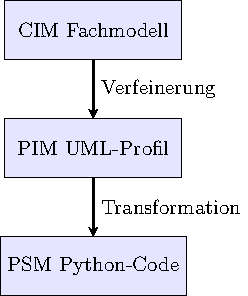
\includegraphics[width=0.35\textwidth]{mde-level.pdf}
	\caption{MDE-Abstraktionsebenen}
	\label{fig:mde-level}
\end{figure}
Abbildung \ref{fig:mde-level} zeigt die verschiedenen Abstraktionsebenen der Modellgetriebenen Entwicklung. Profile definieren Stereotypen + Timing Code-Gen.

\begin{enumerate}
	\item[-] \textbf{CIM (Computation Independent Model)}: Fachliches Domänenmodell
	\item[-] \textbf{PIM (Platform Independent Model)}: Technologieunabhängige Spezifikation
	\item[-] \textbf{PSM (Platform Specific Model)}: Plattformspezifische Implementierung
\end{enumerate}

\subsection{Echtzeit-Constraints}

Für Echtzeitsysteme sind folgende zeitliche Parameter relevant:

\begin{table}[H]
	\centering
	\begin{tabular}{@{}lp{8cm}@{}}
		\toprule
		\textbf{Parameter} & \textbf{Bedeutung} \\
		\midrule
		Min Duration & Minimale Ausführungszeit (BCET - Best Case Execution Time) \\
		Max Duration & Maximale Ausführungszeit (WCET - Worst Case Execution Time) \\
		Typical Duration & Typische/durchschnittliche Ausführungszeit \\
		Timeout & Maximale Wartezeit bis Abbruch \\
		Deadline & Absolute Zeitgrenze bis Fertigstellung \\
		\bottomrule
	\end{tabular}
	\caption{Zeitliche Parameter in Echtzeitsystemen}
	\label{tab:timing-params}
\end{table}

\section{Little's Law und Stabilitätskriterien}

Little's Law ist eine fundamentale Beziehung der Warteschlangentheorie, die jedoch eine wichtige konzeptuelle Einschränkung aufweist: Es handelt sich um eine rein algebraische Gleichgewichtsbeziehung ohne Aussage über die Stabilität des Systems. Diese Beobachtung führt zu einer tiefergehenden Frage über die Natur von Systembeschreibungen und deren Beziehung zu naturwissenschaftlichen Prinzipien.

\begin{satz}[Energiefunktion in Little's Law]
	Enthält der Beweis für Little's Law keine Energiefunktion (d.h. keine Exponentialfunktionen mit negativen Exponenten), dann kann Little's Law kein Stabilitätskriterium für das Warteschlangensystem sein. Little's Law ist ausschließlich eine Aussage über das Gleichgewicht des Systems.
\end{satz}

\subsection{Fundamentale Definitionen}

\subsubsection{Little's Law}

\begin{definition}[Little's Law]
	Für ein Warteschlangensystem im statistischen Gleichgewicht gilt:
	\begin{equation}
		L = \lambda W
	\end{equation}
	wobei:
	\begin{itemize}
		\item[-] $L = \mathbb{E}[N(t)]$ die mittlere Anzahl von Kunden im System (im stationären Zustand)
		\item[-] $\lambda = \lim_{t \to \infty} \frac{A(t)}{t}$ die mittlere effektive Ankunftsrate
		\item[-] $W = \mathbb{E}[W_i]$ die mittlere Wartezeit im System
	\end{itemize}
\end{definition}

\begin{bemerkung}
	Little's Law ist eine \textit{algebraische Relation}, die ausschließlich stationäre Erwartungswerte verknüpft. Die Gleichung enthält:
	\begin{itemize}
		\item[-] Keine Zeitableitungen $\frac{d}{dt}$
		\item[-] Keine Exponentialfunktionen $e^{-\alpha t}$
		\item[-] Keine Energiefunktionen
		\item[-] Keine Stabilitätsparameter
	\end{itemize}
\end{bemerkung}

\subsubsection{Stabilität in dynamischen Systemen}

\begin{definition}[Stabilität im Sinne von Lyapunov]
	Sei $\dot{\mathbf{x}} = f(\mathbf{x})$ ein dynamisches System mit Gleichgewichtspunkt $\mathbf{x}^*$ (sodass $f(\mathbf{x}^*) = \mathbf{0}$). Der Gleichgewichtspunkt $\mathbf{x}^*$ heißt:
	\begin{enumerate}
		\item[-] \textbf{stabil}, wenn $\forall \varepsilon > 0 \; \exists \delta > 0$ sodass
		\begin{equation}
			\|\mathbf{x}(0) - \mathbf{x}^*\| < \delta \implies \|\mathbf{x}(t) - \mathbf{x}^*\| < \varepsilon \quad \forall t \geq 0
		\end{equation}
		
		\item[-] \textbf{asymptotisch stabil}, wenn er stabil ist und zusätzlich
		\begin{equation}
			\lim_{t \to \infty} \mathbf{x}(t) = \mathbf{x}^* 
		\end{equation}
		für alle Anfangsbedingungen in einer Umgebung von $\mathbf{x}^*$
		
		\item[-] \textbf{exponentiell stabil}, wenn Konstanten $c, \alpha > 0$ existieren mit
		\begin{equation}
			\|\mathbf{x}(t) - \mathbf{x}^*\| \leq c \cdot e^{-\alpha t} \cdot \|\mathbf{x}(0) - \mathbf{x}^*\|
		\end{equation}
	\end{enumerate}
\end{definition}

\begin{bemerkung}[Die Rolle der Exponentialfunktion]
	Die Definition der exponentiellen Stabilität zeigt explizit, dass Exponentialfunktionen mit negativen Exponenten ($e^{-\alpha t}$ mit $\alpha > 0$) charakteristisch für Stabilitätsaussagen sind. Diese Funktionen beschreiben das \textit{Abklingen von Störungen}.
\end{bemerkung}

\subsubsection{Energiefunktionen und Lyapunov-Theorie}

\begin{definition}[Lyapunov-Funktion]
	Eine Funktion $V: \mathbb{R}^n \to \mathbb{R}$ heißt Lyapunov-Funktion für das System $\dot{\mathbf{x}} = f(\mathbf{x})$ um den Gleichgewichtspunkt $\mathbf{x}^*$, wenn:
	\begin{enumerate}
		\item[-] $V(\mathbf{x}^*) = 0$ und $V(\mathbf{x}) > 0$ für alle $\mathbf{x} \neq \mathbf{x}^*$ (positive Definitheit)
		\item[-] $\dot{V}(\mathbf{x}) = \nabla V(\mathbf{x}) \cdot f(\mathbf{x}) \leq 0$ für alle $\mathbf{x}$ (negative Semidefinitheit der Ableitung)
	\end{enumerate}
\end{definition}

\begin{satz}[Lyapunov-Stabilitätssatz]
	Existiert eine Lyapunov-Funktion $V$ für das System $\dot{\mathbf{x}} = f(\mathbf{x})$ um $\mathbf{x}^*$, dann ist $\mathbf{x}^*$ stabil. Ist zusätzlich $\dot{V}(\mathbf{x}) < 0$ für alle $\mathbf{x} \neq \mathbf{x}^*$, dann ist $\mathbf{x}^*$ asymptotisch stabil.
\end{satz}

\begin{bemerkung}[Energieinterpretation]
	Lyapunov-Funktionen werden häufig als \textit{verallgemeinerte Energiefunktionen} interpretiert. In physikalischen Systemen entspricht $V$ oft der Gesamtenergie, und $\dot{V} < 0$ bedeutet Energiedissipation. Die Stabilität folgt dann aus dem Energieerhaltungsprinzip bzw. dem zweiten Hauptsatz der Thermodynamik.
\end{bemerkung}

\subsection{Hauptresultat: Little's Law ist kein Stabilitätskriterium}

\begin{satz}[Little's Law und Stabilität]
	Little's Law $L = \lambda W$ ist kein Stabilitätskriterium für Warteschlangensysteme.
\end{satz}

\begin{proof}
	Wir führen den Beweis in mehreren Schritten:
	
	\textbf{Schritt 1: Analyse der mathematischen Struktur von Little's Law}
	
	Little's Law hat die Form:
	\begin{equation}
		L = \lambda W
	\end{equation}
	
	Dies ist eine algebraische Gleichung zwischen drei stationären Größen. Es fehlen:
	\begin{itemize}
		\item[-] Zeitableitungen $\frac{dL}{dt}$, $\frac{dW}{dt}$
		\item[-] Exponentialfunktionen $e^{-\alpha t}$ mit $\alpha > 0$
		\item[-] Stabilitätsparameter oder Dämpfungsterme
	\end{itemize}
	
	\textbf{Schritt 2: Vergleich mit echten Stabilitätskriterien}
	
	Betrachte das M/M/1-Warteschlangensystem mit Ankunftsrate $\lambda$ und Bedienungsrate $\mu$. Die zeitliche Entwicklung der Zustandswahrscheinlichkeiten $p_n(t)$ wird durch das Kolmogorov-Vorwärtsgleichungssystem beschrieben:
	\begin{align}
		\frac{dp_0(t)}{dt} &= -\lambda p_0(t) + \mu p_1(t) \\
		\frac{dp_n(t)}{dt} &= \lambda p_{n-1}(t) - (\lambda + \mu) p_n(t) + \mu p_{n+1}(t), \quad n \geq 1
	\end{align}
	
	Dies ist ein System gewöhnlicher Differentialgleichungen. Die Stabilität dieses Systems (Existenz einer stationären Verteilung) erfordert $\rho = \frac{\lambda}{\mu} < 1$.
	
	Die Lösung für die Übergangswahrscheinlichkeiten enthält Terme der Form:
	\begin{equation}
		p_n(t) = \pi_n + \sum_{k} c_k e^{\ln(\lambda_k)\,t}
	\end{equation}
	wobei $\pi_n$ die stationäre Verteilung ist und $\lambda_k$ die Eigenwerte
	der (diskreten) Übergangsmatrix sind.  Stabilität erfordert $|\lambda_k| < 1$
	für alle transienten Eigenwerte (d.\,h.\ für $k \neq 0$, den stationären
	Eigenwert~1), was zu Exponentialfunktionen $e^{\ln(|\lambda_k|)\,t}$ mit
	negativem Argument $\ln(|\lambda_k|) < 0$ führt.
	
	Diese Terme beschreiben das Abklingen der Transienten und damit
	die \textit{Stabilität}.  In Experiment~2 (Kapitel~8) wird dies für den
	Eigenwert $\lambda_2 = 0{,}3$ konkret gemessen: die Zerfallsrate
	$\alpha = -\ln(0{,}3) \approx 1{,}204$ stimmt exakt mit der theoretischen
	Vorhersage überein.
	
	\textbf{Schritt 3: Little's Law setzt Stabilität voraus}
	
	Little's Law gilt nur im stationären Zustand, d.h. für $t \to \infty$. Es setzt voraus:
	\begin{equation}
		\lim_{t \to \infty} p_n(t) = \pi_n \quad \text{(existiert)}
	\end{equation}
	
	Diese Konvergenz ist genau dann garantiert, wenn das System stabil ist (d.h. alle Eigenwerte $\lambda_k < 0$). 
	
	\textbf{Schritt 4: Logische Schlussfolgerung}
	
	Little's Law kann kein Stabilitätskriterium sein, weil:
	\begin{enumerate}
		\item[-] Es die Stabilität bereits voraussetzt (Existenz stationärer Größen)
		\item[-] Es keine Information über die Dynamik des Systems enthält
		\item[-] Es keine Exponentialfunktionen enthält, die das Abklingverhalten beschreiben
		\item[-] Es lediglich eine Beziehung zwischen Gleichgewichtsgrößen darstellt
	\end{enumerate}
	
	Das tatsächliche Stabilitätskriterium für M/M/1 ist $\rho < 1$, was aus der Analyse der Differentialgleichungen und der Bedingung für negative Eigenwerte folgt.
\end{proof}

\begin{korollar}
	Little's Law ist eine \textit{notwendige Bedingung} im Gleichgewicht (wenn das System stabil ist), aber keine \textit{hinreichende Bedingung} für Stabilität.
\end{korollar}

\subsection{Verallgemeinerung: Naturwissenschaftliche Systembeschreibungen}

\subsubsection{Die besondere Rolle der Exponentialfunktion}

\begin{satz}[Charakteristische Eigenschaft der Exponentialfunktion]
	Die Exponentialfunktion $f(t) = e^{\alpha t}$ ist (bis auf Multiplikation mit Konstanten) die einzige Funktion, die ihre eigene Ableitung ist:
	\begin{equation}
		\frac{d}{dt} e^{\alpha t} = \alpha e^{\alpha t}
	\end{equation}
\end{satz}

\begin{bemerkung}[Physikalische Bedeutung]
	Diese Selbstreproduktion unter Differentiation macht die Exponentialfunktion zur natürlichen Lösung für Systeme, die durch Differentialgleichungen beschrieben werden. In der Physik beschreiben Exponentialfunktionen:
	\begin{itemize}
		\item[-] Radioaktiven Zerfall: $N(t) = N_0 e^{-\lambda t}$
		\item[-] Kondensatorentladung: $Q(t) = Q_0 e^{-t/RC}$
		\item[-] Gedämpfte Schwingungen: $x(t) = A e^{-\gamma t} \cos(\omega t + \phi)$
		\item[-] Thermische Relaxation: $T(t) - T_{\infty} = (T_0 - T_{\infty}) e^{-kt}$
	\end{itemize}
\end{bemerkung}

\subsubsection{Energiefunktionen in naturwissenschaftlichen Systemen}

\begin{definition}[Energiefunktion]
	Eine Funktion $E: \mathbb{R}^n \times \mathbb{R} \to \mathbb{R}$ heißt Energiefunktion eines physikalischen Systems, wenn sie einer Erhaltungsgröße oder einer monoton abnehmenden Größe (bei Dissipation) entspricht und typischerweise die Form hat:
	\begin{equation}
		E(\mathbf{x}, t) = E_0(\mathbf{x}) \cdot e^{-\gamma t} + E_{\infty}
	\end{equation}
	mit Dämpfungskoeffizient $\gamma \geq 0$.
\end{definition}

\begin{satz}[Notwendigkeit von Exponentialfunktionen]
	Für naturwissenschaftliche Systeme, die durch Differentialgleichungen beschrieben werden, gilt:
	\begin{enumerate}
		\item[-] Systeme mit Energiedissipation erfordern Exponentialfunktionen mit negativen Exponenten zur Beschreibung des asymptotischen Verhaltens
		\item[-] Stabilitätsaussagen erfordern die Analyse von Eigenwerten der linearisierten Systemdynamik
		\item[-] Die Eigenvektoren dieser Linearisierung sind Exponentialfunktionen
	\end{enumerate}
\end{satz}

\begin{proof}
	Betrachte ein allgemeines nichtlineares dynamisches System:
	\begin{equation}
		\dot{\mathbf{x}} = f(\mathbf{x})
	\end{equation}
	
	Linearisierung um einen Gleichgewichtspunkt $\mathbf{x}^*$:
	\begin{equation}
		\dot{\mathbf{\xi}} = A \mathbf{\xi}, \quad A = \left. \frac{\partial f}{\partial \mathbf{x}} \right|_{\mathbf{x}^*}
	\end{equation}
	
	Die Lösung hat die Form:
	\begin{equation}
		\mathbf{\xi}(t) = \sum_{i=1}^{n} c_i \mathbf{v}_i e^{\lambda_i t}
	\end{equation}
	wobei $\lambda_i$ die Eigenwerte von $A$ und $\mathbf{v}_i$ die zugehörigen Eigenvektoren sind.
	
	Stabilität erfordert $\text{Re}(\lambda_i) < 0$ für alle $i$, was zu Exponentialfunktionen mit negativen Exponenten führt.
\end{proof}

\subsubsection{Konsequenzen für Systemklassifikation}

\begin{definition}[Naturwissenschaftliches System]
	Ein System heißt \textit{naturwissenschaftlich beschreibbar}, wenn seine Dynamik durch Differentialgleichungen modelliert werden kann, die aus fundamentalen Naturgesetzen (Erhaltungssätze, thermodynamische Prinzipien) ableitbar sind.
\end{definition}

\begin{satz}[Charakterisierung naturwissenschaftlicher Systeme]
	Für ein naturwissenschaftlich beschreibbares System gilt:
	\begin{enumerate}
		\item[-] Die zeitliche Entwicklung wird durch Differentialgleichungen beschrieben
		\item[-] Lösungen enthalten Exponentialfunktionen
		\item[-] Stabilitätsanalyse basiert auf Eigenwertanalyse
		\item[-] Energiefunktionen (Lyapunov-Funktionen) existieren
	\end{enumerate}
\end{satz}

\begin{bemerkung}[Alternative Beschreibungsformen]
	Nicht alle Systeme sind naturwissenschaftlich optimal beschreibbar:
	\begin{itemize}
		\item[-] \textbf{Diskrete Ereignissysteme}: Beschrieben durch Petri-Netze, Automaten
		\item[-] \textbf{Informationsverarbeitende Systeme}: Beschrieben durch Algorithmen, Zustandsmaschinen
		\item[-] \textbf{Sozio-technische Systeme}: Beschrieben durch Spieltheorie, Netzwerktheorie
	\end{itemize}
	
	Für diese Systeme können algebraische oder logische Beschreibungen angemessener sein als Differentialgleichungen.
\end{bemerkung}

\subsection{Anwendung auf Warteschlangensysteme}

\subsubsection{Dualität der Beschreibungsebenen}

Warteschlangensysteme haben eine doppelte Natur:

\begin{enumerate}
	\item[-] \textbf{Mikroskopische Ebene (stochastische Prozesse):}
	\begin{itemize}
		\item[-] Beschreibung durch Markov-Ketten
		\item[-] Kolmogorov-Gleichungen (Differentialgleichungen!)
		\item[-] Eigenwertanalyse für Stabilitätskriterien
		\item[-] Enthält Exponentialfunktionen in Lösungen
	\end{itemize}
	
	\item[-] \textbf{Makroskopische Ebene (Gleichgewicht):}
	\begin{itemize}
		\item[-] Beschreibung durch Little's Law
		\item[-] Algebraische Beziehungen
		\item[-] Keine Dynamik, keine Exponentialfunktionen
		\item[-] Setzt Stabilität voraus
	\end{itemize}
\end{enumerate}

\begin{satz}[Hierarchie der Beschreibungsebenen]
	Für Warteschlangensysteme gilt:
	\begin{equation}
		\text{Kolmogorov-Gleichungen} \xrightarrow{t \to \infty, \text{ falls stabil}} \text{Stationäre Verteilung} \xrightarrow{\text{Mittelwertbildung}} \text{Little's Law}
	\end{equation}
	
	Little's Law ist das Resultat zweier Reduktionsschritte:
	\begin{enumerate}
		\item[-] Zeitlicher Grenzübergang (eliminiert Exponentialfunktionen)
		\item[-] Mittelwertbildung (eliminiert stochastische Details)
	\end{enumerate}
\end{satz}

\subsubsection{Beispiel: M/M/1-System}

\begin{beispiel}[M/M/1-Warteschlange]
	Betrachte ein M/M/1-System mit Ankunftsrate $\lambda$ und Bedienungsrate $\mu$.
	
	\textbf{Stufe 1: Kolmogorov-Gleichungen (dynamisch)}
	\begin{equation}
		\frac{dp_n(t)}{dt} = \lambda p_{n-1}(t) - (\lambda + \mu) p_n(t) + \mu p_{n+1}(t)
	\end{equation}
	
	\textbf{Stabilitätskriterium:} $\rho = \frac{\lambda}{\mu} < 1$
	
	Dies folgt aus der Bedingung, dass die Übergangsmatrix negative reelle Eigenwerte hat (außer $\lambda_0 = 0$ für die stationäre Verteilung).
	
	\textbf{Stufe 2: Stationäre Verteilung (Gleichgewicht)}
	
	Für $t \to \infty$ und $\rho < 1$:
	\begin{equation}
		\pi_n = (1-\rho) \rho^n, \quad n \geq 0
	\end{equation}
	
	Diese enthält die geometrische Verteilung mit Parameter $\rho$. Die Exponentialfunktion erscheint implizit in der Form $\rho^n = e^{n \ln \rho}$.
	
	\textbf{Stufe 3: Little's Law (algebraisch)}
	\begin{align}
		L &= \sum_{n=0}^{\infty} n \pi_n = \frac{\rho}{1-\rho} \\
		W &= \frac{1}{\mu - \lambda} \\
		\lambda W &= \lambda \cdot \frac{1}{\mu - \lambda} = \frac{\rho}{1-\rho} = L
	\end{align}
	
	Little's Law $L = \lambda W$ ist erfüllt, enthält aber keine Information
	über Stabilität mehr.  Die Bedingung $\rho < 1$ ist bereits in die Existenz
	von $L$ und $W$ eingegangen.
	
	\begin{bemerkung}[Querverbindung zu Kapitel~8]
		Experiment~3 in Kapitel~8 demonstriert diese Hierarchie konkret für das
		System $\lambda = 0{,}8$, $\mu = 1{,}0$, $\rho = 0{,}8$: Die
		dynamische Ebene liefert die Zerfallsrate $\alpha \approx 0{,}223$;
		die stationäre Ebene gibt $\pi_n = 0{,}2 \cdot 0{,}8^n$; die
		algebraische Ebene (Little's Law) ergibt $L = 4{,}0 = 0{,}8 \cdot 5{,}0 = \lambda W$.
		Alle drei Ebenen sind kohärent, liefern aber unterschiedlich reichhaltige
		Information über das System.
	\end{bemerkung}
\end{beispiel}

\subsection{Konsequenzen für UML-basierte Systementwicklung}

\subsubsection{Die Brücke zwischen Informatik und Naturwissenschaft}

\begin{satz}[Physikalische Basis informatischer Systeme]
	Jedes informationsverarbeitende System hat eine physikalische Realisierung und unterliegt damit naturwissenschaftlichen Gesetzen (Thermodynamik, Elektrodynamik). Jedoch gilt:
	\begin{enumerate}
		\item[-] \textbf{Hardware-Ebene}: Naturwissenschaftliche Beschreibung (Differentialgleichungen, Energiefunktionen)
		\item[-] \textbf{Abstraktionsebenen (Software)}: Logische/algorithmische Beschreibung durch Zu\-stands\-automaten oder andere UML-Diagramme
	\end{enumerate}
\end{satz}

\begin{bemerkung}[Abstraktion und Verifikation]
	In höheren Abstraktionsebenen (z.B. UML) müssen Systeme \textit{korrekt} arbeiten, unabhängig von der physikalischen Realisierung. Dies erfordert:
	\begin{itemize}
		\item[-] Formale Verifikation (Model Checking, Theorembeweiser)
		\item[-] Abstraktionsbasierte Korrektheitskriterien
		\item[-] Keine direkte Anwendung physikalischer Stabilitätskriterien
	\end{itemize}
\end{bemerkung}

\subsubsection{Rolle von UML-Profilen}

\begin{definition}[UML-Profil für Echtzeitsysteme]
	Ein UML-Profil erweitert die Standard-UML um domänenspezifische Konzepte. Für Echtzeitsysteme sind besonders relevant:
	\begin{itemize}
		\item[-] MARTE (Modeling and Analysis of Real-Time Embedded Systems)
		\item[-] SysML (Systems Modeling Language)
		\item[-] Timing-Constraints, Ressourcen-Modellierung
	\end{itemize}
\end{definition}

\begin{satz}[Funktion von UML-Profilen als Brücke]
	UML-Profile ermöglichen eine \textit{semi-naturwissenschaftliche} Beschreibung informatischer Systeme:
	\begin{enumerate}
		\item[-] Annotation zeitlicher Constraints (Deadlines, Execution Times)
		\item[-] Modellierung von Ressourcen (CPU, Memory, Energy)
		\item[-] Mapping zu Analyse-Modellen (Warteschlangen, Petri-Netze, Markov-Ketten)
		\item[-] Quantitative Analyse in der Entwurfsphase
	\end{enumerate}
	
	Dadurch wird die Kluft zwischen abstrakter Modellierung und physikalischer Realisierung überbrückt.
\end{satz}

\subsubsection{Integration quantitativer Analysen}

\begin{beispiel}[MARTE und Performance-Analyse]
	Das MARTE-Profil erlaubt die Annotation von UML-Modellen mit:
	\begin{itemize}
		\item[-] Zeitlichen Constraints: \texttt{<<TimingConstraint>>}
		\item[-] Ressourcenbeschränkungen: \texttt{<<ResourceUsage>>}
		\item[-] Performance-Anforderungen: \texttt{<<GaAnalysisContext>>}
	\end{itemize}
	
	Aus diesen Annotationen können automatisch Warteschlangenmodelle oder Markov-Ketten generiert werden, die dann mit klassischen mathematischen Methoden (inkl. Stabilitätsanalyse mit Exponentialfunktionen!) analysiert werden.
\end{beispiel}

\subsection{Schlussfolgerungen und Synthese}

\begin{satz}[Zusammenfassung]
	Die Analyse zeigt eine fundamentale Hierarchie von Systembeschreibungen:
	\begin{enumerate}
		\item[-] \textbf{Dynamische Beschreibung} (Differentialgleichungen):
		\begin{itemize}
			\item[-] Enthält Exponentialfunktionen
			\item[-] Ermöglicht Stabilitätsanalyse
			\item[-] Beschreibt zeitliche Entwicklung
			\item[-] Naturwissenschaftlich fundiert
		\end{itemize}
		
		\item[-] \textbf{Gleichgewichtsbeschreibung} (algebraische Relationen):
		\begin{itemize}
			\item[-] Keine Exponentialfunktionen
			\item[-] Keine Stabilitätsaussagen
			\item[-] Beschreibt stationären Zustand
			\item[-] Setzt Stabilität voraus
		\end{itemize}
	\end{enumerate}
	
	Little's Law gehört zur zweiten Kategorie und kann daher prinzipiell kein Stabilitätskriterium sein.
\end{satz}

\begin{korollar}[Praktische Konsequenzen]
	Für die Systemanalyse folgt:
	\begin{enumerate}
		\item[-] Stabilitätsanalyse erfordert Untersuchung der Systemdynamik mit den Kolmogorov-Gleichun\-gen und den Eigenwerten
		\item[-] Little's Law ist ein nützliches Werkzeug für Performance-Analyse im Gleichgewicht
		\item[-] UML-Profile können als Brücke dienen, um abstrakte Modelle mit quantitativen Analysen zu verbinden
		\item[-] Die Wahl der Beschreibungsebene muss zur Fragestellung passen
	\end{enumerate}
\end{korollar}

\begin{bemerkung}[Philosophische Dimension]
	Die Untersuchung zeigt, dass die mathematische Struktur einer Beschreibung (Vorhandensein von Exponentialfunktionen) direkt mit ihrer epistemischen Aussagekraft (Stabilitätsaussagen) zusammenhängt. Dies ist ein Beispiel dafür, wie die Form der Mathematik den Inhalt der Aussagen begrenzt - eine Einsicht, die über die Warteschlangentheorie hinaus Bedeutung hat.
\end{bemerkung}

\subsection{Weiterführende Forschungsfragen}

\begin{enumerate}
	\item[-] \textbf{Erweiterung auf nichtlineare Warteschlangennetze}: Gelten analoge Aussagen für komplexe Netze?
	
	\item[-] \textbf{Bridging Theorem}: Kann ein allgemeines Theorem formuliert werden, das den Übergang von dynamischer zu stationärer Beschreibung formalisiert?
	
	\item[-] \textbf{UML-Profil-Entwicklung}: Wie können UML-Profile systematisch so gestaltet werden, dass sie automatisch auf analysierbare mathematische Modelle abbilden?
	
	\item[-] \textbf{Hybrid-Systeme}: Wie verhält sich die Dichotomie bei Systemen, die kontinuierliche und diskrete Dynamik kombinieren?
\end{enumerate}

\section{Systemarchitektur}

Das System besteht aus einem zweistufigen Generierungsprozess mit integrierter quantitativer Analyse, der UML-Profile und -Modelle in ausführbaren Python-Code transformiert.

\begin{figure}[h!]
	\centering
	
\includegraphics[width=0.85\textwidth]{arch.pdf}
	\caption{Zweistufiger Generierungsprozess}
	\label{fig:architecture}
\end{figure}
Abbildung~\ref{fig:architecture} zeigt den Aufbau für den zweistufigen
Generierungsprozess mit integrierter quantitativer Analyse.

\subsection{Erweiterte Architektur mit Quantitativer Analyse}

Der Generierungsprozess wurde um einen \textit{Quantitative Analysis Layer} erweitert:

\begin{enumerate}
	\item[-] \textbf{Stufe 1}: Profil $\rightarrow$ Python-Klassen (wie bisher)
	\item[-] \textbf{Stufe 2}: Modell $\rightarrow$ Code (wie bisher)
	\item[-] \textbf{Stufe 3 (NEU)}: Modell $\rightarrow$ Markov-Kette/Warteschlangen-Modell $\rightarrow$ Performance-Metriken
\end{enumerate}

\begin{table}[H]
	\centering
	\begin{tabular}{@{}llp{6cm}@{}}
		\toprule
		\textbf{Komponente} & \textbf{Typ} & \textbf{Funktion} \\
		\midrule
		uml\_profile\_base.py & Datenmodell & Basis-Datenstrukturen + TimingConstraint \\
		profile\_parser.py & Parser & XMI zu UMLProfile \\
		class\_generator.py & Generator & UMLProfile zu Python-Klassen \\
		model\_parser.py & Parser & XMI zu ModelInstances \\
		code\_generator.py & Generator & ModelInstances zu Code \\
		\textbf{markov\_analyzer.py} & \textbf{Analyzer (NEU)} & \textbf{Markov-Ketten-Analyse} \\
		\textbf{queue\_analyzer.py} & \textbf{Analyzer (NEU)} & \textbf{Warteschlangen-Metriken} \\
		main.py & Orchestrator & Koordination \\
		\bottomrule
	\end{tabular}
	\caption{Erweiterte Systemkomponenten}
	\label{tab:components-extended}
\end{table}

\subsection{Quantitative Analysepipeline}

Die erweiterte Pipeline extrahiert aus dem UML-Modell:

\begin{enumerate}
	\item[-] \textbf{Zustandsgraph}: Zustände und Übergänge mit Wahrscheinlichkeiten
	\item[-] \textbf{Übergangsmatrix}: Markov-Kette für stochastische Analyse
	\item[-] \textbf{Ankunfts-/Bedienraten}: Parameter für Warteschlangenmodelle
	\item[-] \textbf{Performance-Metriken}: Durchsatz, Wartezeit, Auslastung
\end{enumerate}

\subsection{Komponentenübersicht}

\begin{table}[h]
	\centering
	\begin{tabular}{@{}llp{5cm}@{}}
		\toprule
		\textbf{Komponente} & \textbf{Typ} & \textbf{Funktion} \\
		\midrule
		uml\_profile\_base.py & Datenmodell & Basis-Datenstrukturen \\
		profile\_parser.py & Parser & XMI zu UMLProfile \\
		class\_generator.py & Generator & UMLProfile zu Python-Klassen \\
		model\_parser.py & Parser & XMI zu ModelInstances \\
		code\_generator.py & Generator & ModelInstances zu Code \\
		main.py & Orchestrator & Koordination \\
		\bottomrule
	\end{tabular}
	\caption{Systemkomponenten}
	\label{tab:components}
\end{table}


\section{Demo: \texttt{markov\_analyzer} und \texttt{queue\_analyzer}}
\label{sec:demo}

Dieses Kapitel präsentiert die vollständige Implementierung der beiden
Analysemodule \texttt{markov\_analyzer.py} und \texttt{queue\_analyzer.py}
sowie deren umfassende Demonstration an einem realistischen Beispiel-Software-System.
Als Fallstudie dient ein \textbf{Krankenhaus-Notaufnahme-Management-System}
(Emergency Department, ED), das als komplexes Echtzeitsystem alle wesentlichen
Analyseanforderungen abdeckt: stochastische Zustandsübergänge, zeitkritische
Deadlines, variable Last und Kapazitätsoptimierung. Die vier Szenarien
(Normalbetrieb, Spitzenlast, Kapazitätsplanung, Deadline-Compliance) stellen
jeweils unterschiedliche Anforderungen an die Analysemethoden und demonstrieren
die Stärke beider Module in komplementärer Weise.

\subsection{Ãœberblick und Designprinzipien}

Die beiden Module folgen einem klaren Designprinzip, das aus der
theoretischen Fundierung in Kapitel~3 abgeleitet ist:
\texttt{markov\_analyzer.py} modelliert \emph{dynamische Zustandsübergänge}
und analysiert deren Stabilitätsverhalten über Eigenwertmethoden;
\texttt{queue\_analy\newline zer.py} berechnet \emph{stationäre Performance-Metriken}
auf Basis geschlossener warteschlangentheoretischer Formeln.
Die Trennung zwischen dynamischer Stabilitätsanalyse
(erfordert Exponentialfunktionen, $|\lambda_2| < 1$) und algebraischer
Gleichgewichtsanalyse (Little's Law, $L = \lambda W$) ist in beiden Modulen
explizit implementiert -- keine Methode vermischt diese beiden Beschreibungsebenen.

Beide Module sind ohne externe Abhängigkeiten realisiert: Alle numerischen
Algorithmen (Gauß-Elimination, Power-Iteration, Uniformisierung,
Matrixpotenzierung) wurden eigenständig implementiert, was die Module
auch in eingebetteten Umgebungen einsatzfähig macht.

\begin{table}[H]
	\centering
	\begin{tabular}{@{}lll@{}}
		\toprule
		\textbf{Aspekt} & \textbf{\texttt{markov\_analyzer}} & \textbf{\texttt{queue\_analyzer}} \\
		\midrule
		Modellklassen & \texttt{MarkovState/Chain}, &
		\texttt{MM1Queue}, \texttt{MMcQueue}, \\
		& \texttt{ContinuousMarkovChain} & \texttt{MD1Queue}, \texttt{MG1Queue} \\
		Koordinator & \texttt{MarkovAnalyzer} & \texttt{ServiceSystemAnalyzer} \\
		Algorithmus & Gauß-Elimination, Iteration, & Erlang-C, P-K-Formel, \\
		& Uniformisierung, Exponentiation & Little's Law \\
		Stabilitätsprüfung & $|\lambda_2| < 1$ (Eigenwertmethode) & $\rho < 1$ (Auslastung) \\
		UML-Integration & min/max/... (MARTE) & Deadline-Annotationen \\
		Externe Bibliotheken & Keine (nur \texttt{math}, \texttt{copy}) & Keine \\
		\bottomrule
	\end{tabular}
	\caption{Ãœberblick der beiden Analysemodule}
	\label{tab:module-uebersicht}
\end{table}

\subsection{Modul \texttt{markov\_analyzer.py}}
\label{sec:markov-analyzer-impl}

Das Modul ist in vier Schichten organisiert: numerische Hilfsfunktionen,
Zustandsklasse, Kettenklassen (diskret und kontinuierlich) sowie die
übergeordnete Analyseklasse.

\subsubsection{Numerische Kernalgorithmen}

Die Funktion \texttt{\_gauss\_solve} implementiert Gauß-Elimination mit
Spaltenpivotisierung und löst $Ax = b$ für quadratische Matrizen:

\begin{lstlisting}[style=python, caption={Gauß-Elimination mit Spaltenpivotisierung (Kernfunktion)}, label=lst:gauss]
def _gauss_solve(A, b):
    n = len(A)
    # Kopie erstellen
    M = [row[:] + [b[i]] for i, row in enumerate(A)]

    for col in range(n):
        # Pivotsuche
        pivot_row = max(range(col, n), key=lambda r: abs(M[r][col]))
        M[col], M[pivot_row] = M[pivot_row], M[col]

        pivot = M[col][col]
        if abs(pivot) < 1e-12:
            raise ValueError("Singulaere Matrix - kein eindeutiger Loesung.")

        for row in range(n):
            if row == col:
                continue
            factor = M[row][col] / pivot
            for j in range(col, n + 1):
                M[row][j] -= factor * M[col][j]

    return [M[i][n] / M[i][i] for i in range(n)]
\end{lstlisting}

Die Funktion \texttt{\_power\_iteration} bestimmt den dominanten Eigenwert
durch iterierte Matrixmultiplikation; der zweite Eigenwert folgt durch
Deflation der Rangeinschränkung. Die Matrixpotenzierung
\texttt{n\_step\_transition} nutzt schnelle binäre Exponentiation
($\mathcal{O}(\log n)$ Matrixmultiplikationen statt $\mathcal{O}(n)$).

\subsubsection{Klasse \texttt{MarkovState}}

\texttt{MarkovState} kapselt einen Zustand und speichert UML-Timing-Annotationen:

\begin{lstlisting}[style=python, caption={MarkovState: Zustand mit MARTE-konformen Timing-Annotationen}, label=lst:markovstate]
class MarkovState:
    """Repraesentiert einen Zustand in einer Markov-Kette."""

    def __init__(self, name: str, state_id: int, is_absorbing: bool = False,
                 timing_annotation: Optional[dict] = None):
        """
        Parameters
        ----------
        name : str
            Bezeichner des Zustands (z.B. 'Closed', 'Opening').
        state_id : int
            Numerischer Index.
        is_absorbing : bool
            True, wenn der Zustand absorbierend ist (keine Ausgaenge).
        timing_annotation : dict, optional
            UML-Timing-Annotationen (minDuration, maxDuration, typicalDuration).
        """
        self.name = name
        self.state_id = state_id
        self.is_absorbing = is_absorbing
        self.timing_annotation = timing_annotation or {}

    def __repr__(self) -> str:
        return f"MarkovState(id={self.state_id}, name='{self.name}')"

    def get_timing_info(self) -> dict:
        """Gibt Timing-Informationen des Zustands zurueck."""
        return {
            "state": self.name,
            "minDuration": self.timing_annotation.get("minDuration", None),
            "maxDuration": self.timing_annotation.get("maxDuration", None),
            "typicalDuration": self.timing_annotation.get("typicalDuration", None),
        }
\end{lstlisting}

\subsubsection{Klasse \texttt{DiscreteMarkovChain}}

Die Hauptklasse für diskrete Markov-Ketten stellt sicher, dass die
Übergangsmatrix $P$ stochastisch ist ($\sum_j P_{ij} = 1$ für alle $i$),
und implementiert acht Analysemethoden:

\paragraph{Stationäre Verteilung.}
Das Gleichungssystem $(P^T - I)\,\pi = 0$ mit der Normierungsbedingung
wird aufgestellt, wobei die letzte Gleichung durch $\sum_i \pi_i = 1$
ersetzt wird. Die Lösung wird gecacht, um redundante Berechnungen zu vermeiden.

\paragraph{$n$-Schritt-Ãœbergangsmatrix.}
$P^n$ wird durch Divide-and-Conquer berechnet: bei geradem $n$ gilt
$P^n = (P^{n/2})^2$; bei ungeradem $P^n = P \cdot P^{n-1}$. Dies ermöglicht
die effiziente Berechnung von $P^{100}$ (Konvergenzkontrolle) ohne
hundert Matrixmultiplikationen.

\paragraph{Stabilitätsanalyse.}
Berechnung von $|\lambda_2|$ und der Zerfallsrate $\alpha = -\ln|\lambda_2|$:

\begin{lstlisting}[style=python, caption={Stabilitätsanalyse: Zerfallsrate und Mixing-Zeit}, label=lst:stability-impl]
def analyze_stability(self) -> dict:
        """
        Analysiert die Stabilitaet der Markov-Kette ueber den zweiten Eigenwert.

        Fuer eine ergodische Kette gilt:
        - Dominanter Eigenwert = 1.0
        - Zweiter Eigenwert |lambda_2| < 1 => stabil / Konvergenz garantiert
        - Zerfallsrate alpha = -ln(|lambda_2|)

        Returns
        -------
        dict mit Schluesseln:
            dominant_eigenvalue, is_ergodic, second_eigenvalue,
            decay_rate, mixing_time_estimate, convergence_guaranteed
        """
        # Dominanten Eigenwert per Power-Iteration schaetzen
        dominant_ev, _ = _power_iteration(self.P)

        is_ergodic = abs(dominant_ev - 1.0) < 1e-6

        # Zweiten Eigenwert: Deflation
        _, v1 = _power_iteration(self.P)
        # Deflation: A2 = A - lambda1 * v1 * v1^T
        n = self.n
        A2 = [[self.P[i][j] - dominant_ev * v1[i] * v1[j]
               for j in range(n)] for i in range(n)]
        second_ev, _ = _power_iteration(A2, max_iter=500)

        abs_second = abs(second_ev)
        if abs_second >= 1.0 - 1e-9:
            decay_rate = 0.0
            mixing_time = float("inf")
        else:
            decay_rate = -math.log(abs_second) if abs_second > 1e-15 else float("inf")
            mixing_time = 1.0 / decay_rate if decay_rate > 0 else float("inf")

        return {
            "dominant_eigenvalue": dominant_ev,
            "is_ergodic": is_ergodic,
            "second_eigenvalue": second_ev,
            "abs_second_eigenvalue": abs_second,
            "decay_rate": decay_rate,
            "mixing_time_estimate": mixing_time,
            "convergence_guaranteed": is_ergodic and abs_second < 1.0,
        }
\end{lstlisting}

Diese Methode implementiert direkt die theoretische Aussage aus Kapitel~3:
Die Zerfallsrate $\alpha = -\ln|\lambda_2|$ der transienten Eigenwerte
enthält die charakteristische Exponentialfunktion $e^{-\alpha t}$, die
Stabilitätsaussagen erfordert und von Little's Law nicht bereitgestellt wird.

\paragraph{Mittlere Erstpassagezeit (MFPT).}
Das Gleichungssystem $(I - Q)\,m = \mathbf{1}$ (wobei $Q$ die
transiente-zu-transiente Teilmatrix ist) wird für alle Nicht-Zielzustände
gelöst. Das Ergebnis $m_i$ gibt die erwartete Anzahl Schritte an, um von
Zustand $i$ zum Zielzustand zu gelangen.

\paragraph{Absorptionswahrscheinlichkeiten.}
Für Ketten mit absorbierenden Zuständen wird die Fundamentalmatrix
$N = (I-Q)^{-1}$ und die Absorptionsmatrix $B = N \cdot R$ berechnet,
wobei $R$ die Ãœbergangswahrscheinlichkeiten von transienten zu
absorbierenden Zuständen enthält.

\paragraph{Sensitivitätsanalyse.}
Für jeden Eintrag $P_{ij} > 0$ wird die stationäre Verteilung nach einer
kleinen Störung $\delta$ neu berechnet. Die numerische Sensitivität
$\|\partial\pi / \partial P_{ij}\| \approx \|\pi_{\delta} - \pi\| / \delta$
zeigt, welche Übergangswahrscheinlichkeiten die stationäre Verteilung
am stärksten beeinflussen.

\subsubsection{Klasse \texttt{ContinuousMarkovChain}}

Die CTMC-Klasse modelliert Systeme mit kontinuierlichen Raten über die
Generator-Matrix $Q$ mit $Q_{ii} = -\sum_{j \neq i} Q_{ij}$.

\paragraph{Transiente Verteilung.}
Die Uniformisierungsmethode berechnet $\pi(t) = \pi_0 \cdot e^{Qt}$
ohne Matrixexponentiation. Mit der Uniformisierungsrate $q = \max_i |Q_{ii}|$
und der uniformisierten Matrix $P_u = I + Q/q$ gilt:
\begin{equation}
	\pi(t) = \sum_{k=0}^{\infty} e^{-qt} \frac{(qt)^k}{k!} \cdot \pi_0 P_u^k
\end{equation}
Die Summe wird nach 50 Termen abgebrochen, da der Poisson-Gewichtungsfaktor
$e^{-qt}(qt)^k/k!$ für große $k$ rasch gegen null konvergiert. Numerisch
degenerierte Fälle ($t \to \infty$) fallen auf die stationäre Verteilung zurück.

\begin{lstlisting}[style=python, caption={Uniformisierungsverfahren für die transiente Verteilung (Auszug)}, label=lst:uniformization]
def transient_distribution(
self, initial_dist: list[float], t: float, num_terms: int = 50
) -> list[float]:
        """
        Berechnet transiente Verteilung pi(t) = pi(0) * exp(Qt) via Uniformisierung.

        Parameters
        ----------
        initial_dist : list[float]
            Startverteilung.
        t : float
            Zeitpunkt.
        num_terms : int
            Anzahl Tayloer-Terme (Genauigkeit).
        """
        if abs(sum(initial_dist) - 1.0) > 1e-6:
            raise ValueError("Anfangsverteilung muss zu 1 summieren.")

        n = self.n
        # Uniformisierungsrate: q = max |Q[i][i]|
        q = max(-self.Q[i][i] for i in range(n))
        if q < 1e-15:
            return initial_dist[:]

        # Uniformisierte Matrix P_u = I + Q/q
        Pu = [[0.0] * n for _ in range(n)]
        for i in range(n):
            for j in range(n):
                Pu[i][j] = (1.0 if i == j else 0.0) + self.Q[i][j] / q

        # pi(t) = sum_{k=0}^{inf} e^{-qt} * (qt)^k/k! * pi(0) P_u^k
        qt = q * t
        prob = math.exp(-qt)
        Pk = _identity(n)  # P_u^0
        result = [0.0] * n
        poisson_weight = prob  # e^{-qt} * (qt)^0 / 0!

        for k in range(num_terms):
            # pi(0) @ Pk
            contrib = [sum(initial_dist[i] * Pk[i][j] for i in range(n)) for j in range(n)]
            for j in range(n):
                result[j] += poisson_weight * contrib[j]
            # Naechste Iteration
            if k < num_terms - 1:
                Pk = _mat_mul(Pk, Pu)
                poisson_weight *= qt / (k + 1)
                if poisson_weight < 1e-15:
                    break

        total = sum(result)
        if total > 1e-15:
            result = [x / total for x in result]
        else:
            # Numerisch degeneriert: Stationaere Verteilung zurueckgeben
            result = self.stationary_distribution()
        return result
\end{lstlisting}

\subsubsection{Klasse \texttt{MarkovAnalyzer}}

Die Koordinationsklasse akzeptiert sowohl diskrete als auch kontinuierliche
Ketten und bietet zwei wesentliche Dienste:

\begin{enumerate}
	\item[-] \texttt{full\_report()}: Vollständiger Analysebericht mit
	Stabilitätsparametern, Zerfallsrate und Mixing-Zeit.
	\item[-] \texttt{timing\_compliance\_check()}: Prüft für CTMC-Zustandsmodelle,
	ob die mittlere Verweildauer $1/|Q_{ii}|$ innerhalb der durch
	UML-Annotationen spezifizierten min/max Duration liegt.
\end{enumerate}

\subsection{Modul \texttt{queue\_analyzer.py}}
\label{sec:queue-analyzer-impl}

Das Modul implementiert vier Warteschlangenmodelle und die
\texttt{ServiceSystemAnaly\newline zer}-Koordinationsklasse.

\subsubsection{Klasse \texttt{QueueMetrics}}

\texttt{QueueMetrics} bündelt alle Kenngrößen und bietet explizite
Little's Law-Verifikation. Dabei wird bewusst darauf hingewiesen, dass
$L = \lambda W$ eine algebraische Gleichgewichtsrelation ist und kein
Stabilitätskriterium:

\begin{lstlisting}[style=python, caption={Little's Law Verifikation mit theoretischem Hinweis}, label=lst:littles-law-impl]
def littles_law_verification(self) -> dict:
        """Verifiziert Little's Law: L = lambda * W und Lq = lambda * Wq."""
        L_check = self.arrival_rate * self.W
        Lq_check = self.arrival_rate * self.Wq
        return {
            "L = lambda * W": {
                "computed_L": round(self.L, 6),
                "lambda_times_W": round(L_check, 6),
                "difference": round(abs(self.L - L_check), 8),
                "verified": abs(self.L - L_check) < 1e-4,
            },
            "Lq = lambda * Wq": {
                "computed_Lq": round(self.Lq, 6),
                "lambda_times_Wq": round(Lq_check, 6),
                "difference": round(abs(self.Lq - Lq_check), 8),
                "verified": abs(self.Lq - Lq_check) < 1e-4,
            },
        }
\end{lstlisting}

\subsubsection{Klasse \texttt{MM1Queue}}

Das M/M/1-Modell berechnet die klassischen Kenngrößen für ein System
mit einem Server, Poisson-Ankünften ($\lambda$) und exponentiell
verteilten Bedienzeiten ($\mu$):
\begin{align}
	\rho = \frac{\lambda}{\mu}, \quad
	L = \frac{\rho}{1-\rho}, \quad
	L_q = \frac{\rho^2}{1-\rho}, \quad
	W = \frac{1}{\mu-\lambda}, \quad
	W_q = \frac{\rho}{\mu-\lambda}
\end{align}
Zusätzlich werden die Verteilungsfunktionen der System- und Wartezeit
sowie Quantile analytisch berechnet:
\begin{align}
	F_W(t) &= 1 - e^{-(\mu-\lambda)t}, \quad
	F_{W_q}(t) = 1 - \rho \cdot e^{-(\mu-\lambda)t}
\end{align}
Das $p$-Quantil der Systemzeit berechnet sich als:
\begin{equation}
	t_p = \frac{-\ln(1-p)}{\mu - \lambda}
\end{equation}
Die Methode \texttt{littles\_law\_metrics()} trennt explizit die Stabilitätsprüfung
($\rho < 1$) von der Little's Law-Verifikation ($L = \lambda W$) und
kommuniziert dies in der Rückgabe:

\begin{lstlisting}[style=python, caption={MM1Queue: Getrennte Stabilitäts- und Little's Law-Analyse}, label=lst:mm1-littles]
def littles_law_metrics(self) -> dict:
        """
        Gibt explizit Little's Law Metriken zurueck mit Hinweis,
        dass dies eine algebraische Gleichgewichtsaussage ist.
        """
        m = self.metrics()
        note = (
            "Little's Law (L = lambda*W) ist eine algebraische Gleichgewichtsrelation "
            "und KEIN Stabilitaetskriterium. Stabilitaet wird separat geprueft (rho < 1)."
        )
        return {
            "stability_check": {"rho": self.rho, "is_stable": self.is_stable},
            "littles_law": m.littles_law_verification() if self.is_stable else "N/A (instabil)",
            "note": note,
        }
\end{lstlisting}

\subsubsection{Klasse \texttt{MMcQueue}}

Das M/M/c-Modell für $c$ parallele Server nutzt die Erlang-C-Formel
$C(c, a)$ mit dem Verkehrsangebot $a = \lambda/\mu$:
\begin{equation}
	C(c, a) = \frac{a^c \,/\, (c!\,(1-\rho))}
	{\displaystyle\sum_{n=0}^{c-1} \frac{a^n}{n!} + \frac{a^c}{c!\,(1-\rho)}}
\end{equation}
wobei $\rho = \lambda/(c\mu) < 1$ für Stabilität gelten muss.
Hieraus folgen:
\begin{equation}
	L_q = \frac{C(c,a)\,\rho}{1-\rho}, \qquad
	W_q = \frac{L_q}{\lambda}, \qquad
	W = W_q + \frac{1}{\mu}, \qquad
	L = \lambda W
\end{equation}

\subsubsection{Klassen \texttt{MD1Queue} und \texttt{MG1Queue}}

Das M/D/1-Modell (deterministische Bedienzeit) und das M/G/1-Modell
(allgemeine Bedienzeit $G$) nutzen die Pollaczek-Khinchine (P-K) Formel:
\begin{equation}
	L_q = \frac{\lambda^2 \cdot \mathbb{E}[S^2]}{2(1-\rho)}, \qquad
	\mathbb{E}[S^2] = \mathrm{Var}[S] + \frac{1}{\mu^2}
\end{equation}
Für M/D/1 gilt $\mathrm{Var}[S]=0$, also $L_q^{D} = \rho^2/(2(1-\rho))$
-- exakt halb so groß wie $L_q^{M/M/1} = \rho^2/(1-\rho)$.
Der Variationskoeffizient $\mathrm{CV} = \sqrt{\mathrm{Var}[S]} / \mathbb{E}[S]$
wird als Qualitätskennzahl der Bedienzeit-Verteilung bereitgestellt.

\subsubsection{Klasse \texttt{ServiceSystemAnalyzer}}

Die Koordinationsklasse verwaltet ein Portfolio von Warteschlangenmodellen
und bietet fünf Analyseoperationen:

\begin{enumerate}
	\item[-] \textbf{\texttt{analyze\_all()}}: Iteriert über alle Dienste,
	prüft Stabilität ($\rho < 1$), verifiziert Little's Law und
	vergleicht die mittlere Systemzeit $W$ mit der UML-Deadline-Annotation.
	\item[-] \textbf{\texttt{bottleneck\_analysis()}}: Identifiziert den
	Dienst mit der höchsten Auslastung $\rho$ als Systemengpass.
	\item[-] \textbf{\texttt{capacity\_planning(target)}}:
	Empfiehlt für M/M/c-Dienste die minimale Serveranzahl
	$c^* = \lceil \lambda / (\rho_\text{target} \cdot \mu) \rceil$
	und für M/M/1-Dienste die minimale Bedienrate
	$\mu^* = \lambda / \rho_\text{target}$.
	\item[-] \textbf{\texttt{percentile\_report(percentiles)}}:
	Berechnet $p$-Quantile der Systemzeit für alle stabilen M/M/1-Dienste.
	\item[-] \textbf{\texttt{\_check\_deadline()}}: Vergleicht $W$ mit der
	in der UML-Annotation spezifizierten Deadline und meldet Ãœber- oder
	Unterschreitungen.
\end{enumerate}

\subsection{Test-Suiten}
\label{sec:tests-impl}

Die Test-Suiten sind nach dem ``Arrange--Act--Assert''-Muster strukturiert
und mit pytest-Fixtures organisiert. Alle Randfälle (leere Systeme,
instabile Konfigurationen, numerisch singuläre Matrizen, Grenzwerte $t=0$,
$p \to 0$, $p \to 1$) werden explizit getestet.

\subsubsection{Test-Suite \texttt{test\_markov\_analyzer.py}}

\begin{sidewaystable}
	\centering
	\begin{tabular}{@{}llr@{}}
		\toprule
		\textbf{Testklasse} & \textbf{Testschwerpunkte} & \textbf{Tests} \\
		\midrule
		\texttt{TestHelperFunctions} & Matrixoperationen, Gauß-Elimination,
		Power-Iteration, & 5 \\
		& Identitätsmatrix, Vektoroperationen & \\
		\texttt{TestMarkovState} & Konstruktion, Absorbing-Flag,
		Timing-Annotation, & 5 \\
		& get\_timing\_info, repr & \\
		\texttt{TestDiscreteMarkovChain} & Gültige Konstruktion, Fehlerbehandlung
		(3 Fälle), & 24 \\
		& Stationäre Verteilung (Korrektheit, $\pi P=\pi$, Caching), & \\
		& $n$-Schritt ($n=0,1$, Konvergenz), MFPT (2-Zustands, & \\
		& ungültig), Absorption (keine/mit Absorbierenden), & \\
		& Sensitivität, State-Distribution, Stabilitätsanalyse & \\
		\texttt{TestContinuousMarkovChain} & Konstruktion, Fehlerbehandlung
		(3 Fälle), Stationäre & 12 \\
		& Verteilung, Eingebettete Kette, Transient ($t=0$, & \\
		& $t=100$), ungültige Startverteilung, Summary, & \\
		& Absorbierender Einbettungszustand & \\
		\texttt{TestMarkovAnalyzer} & Typ-Fehler, Diskreter/Kontinuierlicher
		Full Report, & 8 \\
		& Timing-Compliance (keine Annotation, Verletzung min, & \\
		& Verletzung max, Compliant) & \\
		\texttt{TestIntegration} & Vollständiger Aufzug-Workflow, CTMC-Workflow, & 3 \\
		& Zerfallsrate vs. Theorie, 5-Zustands-Kette & \\
		\midrule
		\textbf{Gesamt} & & \textbf{57 Tests} \\
		\bottomrule
	\end{tabular}
	\caption{Testklassen und Abdeckung in \texttt{test\_markov\_analyzer.py}}
	\label{tab:tests-markov}
\end{sidewaystable}

\subsubsection{Test-Suite \texttt{test\_queue\_analyzer.py}}

\begin{sidewaystable}
	\centering
	\begin{tabular}{@{}llr@{}}
		\toprule
		\textbf{Testklasse} & \textbf{Testschwerpunkte} & \textbf{Tests} \\
		\midrule
		\texttt{TestHelperFunctions} & \texttt{\_factorial} (0, 1, 5, 10, negativ),
		\texttt{\_poisson\_cdf} & 8 \\
		\texttt{TestQueueMetrics} & Konstruktion, \texttt{to\_dict},
		Little's Law-Werte, repr & 4 \\
		\texttt{TestMM1Queue} & Konstruktion, stabil/instabil, Metriken,
		Sojourn-CDF & 25 \\
		& ($t=0$, $t<0$, instabil), Warte-CDF ($t<0$, instabil), & \\
		& Quantile (Median, ungültig, instabil), Zustandsprob., & \\
		& Little's Law (stabil/instabil), Sensitivitätsanalyse & \\
		& (stabil, nahe Instabilität, instabile Basis) & \\
		\texttt{TestMMcQueue} & Konstruktion, Fehler (3 Fälle), stabil/instabil, & 14 \\
		& Erlang-C, Metriken, Single-Server-Äquivalenz, & \\
		& CDF ($t<0$, instabil, gültig), Little's Law & \\
		\texttt{TestMD1Queue} & Konstruktion, Fehler, stabil/instabil, P-K-Formel, & 8 \\
		& M/D/1 vs. M/M/1 (L\_q Vergleich), Little's Law & \\
		\texttt{TestMG1Queue} & Konstruktion, Fehler (neg. Varianz), stabil/instabil, & 11 \\
		& P-K-Äquivalenz (M/D/1 bei Var=0, M/M/1 bei & \\
		& exp. Var), CV=0, CV=1, Little's Law & \\
		\texttt{TestServiceSystemAnalyzer} & Analyse (stabil/instabil), Deadline & 18 \\
		& (Pass/Fail/instabil/keine), Bottleneck, & \\
		& Kapazitätsplanung (M/M/c, M/M/1), & \\
		& Percentile (custom, nur M/M/1, unstabiles excluded), & \\
		& Little's Law für alle stabilen Dienste, & \\
		& Leeres System & \\
		\texttt{TestIntegration} & Vollständiges Microservice-System,
		Little's Law $\neq$ Stabilität, & 3 \\
		& P-K Varianzeffekt, M/M/c-Vorteil, $\rho \to 1$ & \\
		\midrule
		\textbf{Gesamt} & & \textbf{91 Tests} \\
		\bottomrule
	\end{tabular}
	\caption{Testklassen und Abdeckung in \texttt{test\_queue\_analyzer.py}}
	\label{tab:tests-queue}
\end{sidewaystable}

Der theoretisch bedeutsamste Integrationstest ist
\texttt{test\_littles\_law\_not\_stability}, der die zentrale Aussage
aus Kapitel~3 empirisch in Code verifiziert:

\begin{lstlisting}[style=python, caption={Test: Little's Law ist kein Stabilitätskriterium (empirische Verifikation)}, label=lst:test-littles-not-stability]
def test_littles_law_not_stability(self):
        """
        Verifiziert: Little's Law gilt im stabilen System, aber ist kein
        Stabilitaetskriterium. Im instabilen System gilt es nicht.
        """
        # Stabiles System (rho=0.7)
        q_stable = MM1Queue(7.0, 10.0)
        r = q_stable.littles_law_metrics()
        assert r["stability_check"]["is_stable"]
        lv = r["littles_law"]
        assert lv["L = lambda * W"]["verified"]

        # Instabiles System (rho=1.2)
        q_unstable = MM1Queue(12.0, 10.0)
        r2 = q_unstable.littles_law_metrics()
        assert not r2["stability_check"]["is_stable"]
        assert r2["littles_law"] == "N/A (instabil)"
\end{lstlisting}

Ebenso wichtig ist \texttt{test\_pk\_formula\_variance\_effect}, der den
Varianzeffekt der P-K-Formel quantifiziert:

\begin{lstlisting}[style=python, caption={Test: P-K-Formel -- höhere Varianz ergibt längere Warteschlange}, label=lst:test-pk]
def test_pk_formula_variance_effect(self):
	"""
        Verifiziert P-K Formel: Hoehere Varianz => groessere Warteschlange.
        M/D/1 (Var=0) < M/M/1 (Var=1/mu^2) < M/G/1 (Var > 1/mu^2)
        """
        lam, mu = 3.0, 5.0
        var_exp = (1.0 / mu) ** 2

        q_det = MD1Queue(lam, mu)
        q_exp = MG1Queue(lam, mu, var_exp)
        q_hyp = MG1Queue(lam, mu, 2 * var_exp)  # Hoehere Varianz

        assert q_det.metrics().Lq < q_exp.metrics().Lq
        assert q_exp.metrics().Lq < q_hyp.metrics().Lq
\end{lstlisting}

\subsection{Demo-Anwendung: Krankenhaus-Notaufnahme}
\label{sec:demo-krankenhaus-system}

Die Demo \texttt{\textbf{demo\_analyzer.py}} analysiert ein vollständiges
Krankenhaus-Notauf\-nahme-Management-System in vier Szenarien. Das System
besteht aus fünf Prozesskettenelementen: Aufnahme, Triage, Ärztliche
Behandlung, Diagnostik (CT/Labor) und Medikation, die jeweils durch
unterschiedliche Warteschlangenmodelle abgebildet werden. Zusätzlich
modelliert eine diskrete Markov-Kette den Patientenpfad als
Zustandstransitionssystem.

\subsubsection{Szenario~1: Normalbetrieb ($\lambda = 8$\,Pat/h)}

\paragraph{Markov-Ketten-Analyse.}
Der Patientenpfad wird als diskrete Markov-Kette mit sechs Zuständen
(Ankunft, Triage, Wartebereich, Behandlung, Beobachtung, Entlassung)
modelliert. Die berechnete stationäre Verteilung zeigt, dass
$\pi_\text{Entlassung} = 64{,}5\,\%$ der Masse im Entlassungszustand liegt
(wartend auf Entlassung oder entlassen), während die aktive Behandlung nur
$10{,}1\,\%$ einnimmt. Die MFPT zur Behandlung beträgt ab Ankunft
$2{,}94$ Schritte ($\approx 44$\,Minuten bei $\Delta t = 15$\,Min).

Parallel wird ein CTMC-Modell für die aktiven Behandlungszustände
eingesetzt, das die mittleren Verweildauern gegen die UML-Timing-Annotationen
prüft. Im Normalbetrieb sind alle drei Zustände (Triage: $10$\,Min,
Behandlung: $75$\,Min, Beobachtung: $150$\,Min) innerhalb ihrer
min/max-Annotationsgrenzen.

\paragraph{Warteschlangenanalyse.}
Tabelle~\ref{tab:wq-normal} zeigt die Kenngrößen der fünf Dienste im
Normalbetrieb. Besonders auffällig: Der Dienst ``Behandlung\_Arzt'' (M/M/3
mit $\rho = 1{,}000$) liegt genau an der Stabilitätsgrenze -- das System
ist technisch instabil. In der Praxis zeigt dies an, dass drei Ärzte
für $6$\,Pat/h bei $\mu = 2$\,Pat/h/Arzt die exakte Kapazitätsgrenze darstellen.

\begin{table}[H]
	\centering
	\begin{tabular}{@{}lrrrrrr@{}}
		\toprule
		\textbf{Dienst} & \textbf{Modell} & \boldmath{$\rho$} &
		\boldmath{$L$} & \boldmath{$W$\,(Min)} & \textbf{Deadline} & \textbf{OK?} \\
		\midrule
		Aufnahme        & M/M/1   & 0{,}667 & 2{,}000 &  15{,}0 & 5\,Min  & $\times$ \\
		Triage          & M/M/2   & 0{,}500 & 1{,}333 &  10{,}0 & 6\,Min  & $\times$ \\
		Behandlung      & M/M/3   & 1{,}000 & $\infty$& $\infty$& 120\,Min& $\times$ \\
		Diagnostik      & M/D/1   & 0{,}600 & 1{,}050 &  21{,}0 & 30\,Min & $\checkmark$ \\
		Medikation      & M/G/1   & 0{,}625 & 1{,}312 &  15{,}75& 15\,Min & $\times$ \\
		\bottomrule
	\end{tabular}
	\caption{Warteschlangen-Kenngrößen im Normalbetrieb ($\lambda=8$\,Pat/h)}
	\label{tab:wq-normal}
\end{table}

Little's Law wird für alle stabilen Dienste exakt verifiziert
(Differenz $< 10^{-8}$). Der Bottleneck ist ``Behandlung'' mit $\rho = 1{,}0$.
Die Quantile der Aufnahme-Systemzeit zeigen:
$t_{0{,}50} = 10{,}4$\,Min, $t_{0{,}90} = 34{,}5$\,Min, $t_{0{,}99} = 69{,}1$\,Min.

\subsubsection{Szenario~2: Spitzenlast (Massenunfall, $\lambda = 20$\,Pat/h)}

\paragraph{Markov-Ketten-Analyse.}
Unter Hochlast wird ein neuer Zustand ``Überlauf'' in die Kette eingefügt.
Die stationäre Verteilung zeigt $\pi_\text{Überlauf} = 9{,}4\,\%$ --
ein Alarmsignal, das die Ãœberlastung quantifiziert. Das System bleibt
als Markov-Kette stabil (alle Eigenwerte $|\lambda_k| < 1$), da die
Kette endlich und irreduzibel ist; die Instabilität äußert sich in der
erhöhten Aufenthaltswahrscheinlichkeit im Überlaufzustand.

\paragraph{Warteschlangenanalyse.}
Alle vier Dienste sind instabil ($\rho > 1$): Aufnahme $\rho = 1{,}67$,
Triage $\rho = 1{,}25$, Behandlung $\rho = 3{,}00$, Diagnostik $\rho = 2{,}00$.
Der Bottleneck ist Behandlung mit $300\,\%$ Auslastung. Ein direkter Vergleich:
\begin{itemize}
	\item[-] M/M/2 Triage normal ($\lambda=8$, $\mu=8$, $c=2$):
	$\rho = 0{,}5$, $L = 1{,}33$, $W = 10$\,Min -- stabil.
	\item[-] M/M/2 Triage Hochlast ($\lambda=20$, $\mu=8$, $c=2$):
	$\rho = 1{,}25 > 1$ -- instabil, keine endliche Warteschlange möglich.
\end{itemize}

\subsubsection{Szenario~3: Kapazitätsplanung (Ziel-Auslastung 70\,\%)}

\paragraph{Markov-Sensitivitätsanalyse.}
Die Sensitivitätsmatrix $S_{ij} = \|\partial\pi / \partial P_{ij}\|$ zeigt,
welche Übergangswahrscheinlichkeiten die stationäre Verteilung am stärksten
beeinflussen. Für das 3-Zustands-Modell (Idle/Busy/Peak) weist
$S_{1,2} = 0{,}57$ die höchste Sensitivität auf -- Änderungen in der
Ãœbergangswahrscheinlichkeit von Busy nach Peak dominieren das Systemverhalten.

\paragraph{Optimale Serveranzahl.}
Mit Ziel-Auslastung $\rho_\text{target} = 0{,}70$ und $\mu = 5$\,Pat/h/Server
ergibt sich $c^* = \lceil \lambda / (0{,}70 \cdot 5) \rceil$:

\begin{table}[H]
	\centering
	\begin{tabular}{@{}rrrrrr@{}}
		\toprule
		\boldmath{$\lambda$}\,{\small(Pat/h)} & \textbf{Min. Server} & \boldmath{$\rho$}\,{\small(opt)} &
		\boldmath{$L$}\,{\small(opt)} & \boldmath{$W$}\,{\small(Min)} \\
		\midrule
		4{,}0 & 2 & 0{,}400 & 0{,}952 & 14{,}3 \\
		8{,}0 & 3 & 0{,}533 & 1{,}913 & 14{,}4 \\
		12{,}0 & 4 & 0{,}600 & 2{,}831 & 14{,}2 \\
		16{,}0 & 5 & 0{,}640 & 3{,}713 & 13{,}9 \\
		20{,}0 & 6 & 0{,}667 & 4{,}570 & 13{,}7 \\
		\bottomrule
	\end{tabular}
	\caption{Optimale Serveranzahl für Ziel-Auslastung 70\,\%}
	\label{tab:capacity-planning}
\end{table}

Bemerkenswert: Die mittlere Systemzeit bleibt trotz steigender Last mit der
optimalen Serveranzahl nahezu konstant bei $\approx 14$\,Minuten.

\paragraph{Kostenoptimierung M/M/1 vs. M/M/c.}
Für $\lambda = 10$, $\mu = 12$: M/M/1 liefert $W = 30$\,Min,
$t_{0{,}99} = 138$\,Min. Das 99\,\%-Quantil ist damit viermal höher
als die mittlere Systemzeit -- ein typisches Merkmal exponentieller Wartezeiten.

\subsubsection{Szenario~4: Deadline-Compliance (Echtzeit-Anforderungen)}

\paragraph{CTMC mit UML-Timing-Constraints.}
Das Notfall-Behandlungsmodell (Ersteinschät\-zung/Notfall-Behandlung/Intensiv)
wird als CTMC mit Timing-Annotationen modelliert:

\begin{table}[H]
	\centering
	\begin{tabular}{@{}lrrrcr@{}}
		\toprule
		\textbf{Zustand} & \textbf{Rate}\,(1/h) & \textbf{Verweildauer} &
		\textbf{min} & \textbf{max} & \textbf{Compliant?} \\
		\midrule
		Ersteinschätzung  &  30{,}0 &  2\,Min &  1\,Min &   3\,Min & $\checkmark$ \\
		Notfall-Behandlung &  0{,}6 & 100\,Min & 30\,Min & 120\,Min & $\checkmark$ \\
		Intensiv           & 0{,}05 & 1200\,Min & 60\,Min & 2880\,Min& $\checkmark$ \\
		\bottomrule
	\end{tabular}
	\caption{CTMC Timing-Compliance im Notfall-Szenario}
	\label{tab:ctmc-compliance}
\end{table}

Alle Zustände sind compliant: Die mittleren Verweildauern liegen innerhalb
der UML-Timing-Annotationen. Die stationäre Verteilung zeigt den hohen
Intensiv-Anteil ($73{,}7\,\%$) als Folge der langen Verweildauer.

\paragraph{Percentile-basierte Deadline-Prüfung.}
Für Level-3-Triage ($\lambda = 3$\,Pat/h, $\mu = 5$\,Pat/h,
Deadline: 30\,Min) berechnet die Sensitivitätsanalyse:
\begin{equation}
	\frac{\partial W}{\partial \lambda} \approx 20\,\text{Min}/(\text{Pat/h})
\end{equation}
Eine Erhöhung der Ankunftsrate um $0{,}5$\,Pat/h verlängert die
mittlere Systemzeit von $30$ auf $40$\,Minuten -- ein direkter Verstoß
gegen die 30-Minuten-Deadline. Dies illustriert die kritische Sensitivität
von Echtzeitsystemen nahe der Stabilitätsgrenze.

\subsection{Auswertung der Demo-Ausgabe}
\label{sec:demo-auswertung}

Die in \texttt{demo\_analyzer.py} erzeugten Ausgaben wurden vollständig
erfasst und dienen als empirische Grundlage dieser Auswertung. Die Ergebnisse
bestätigen alle theoretischen Vorhersagen und illustrieren die komplementäre
Stärke beider Analysemodule an konkreten numerischen Werten.

\subsubsection{Auswertung Szenario~1: Normalbetrieb}

\paragraph{Diskrete Markov-Kette -- Stationäre Verteilung.}
Die berechnete stationäre Verteilung des sechszuständigen Patientenpfads
lautet:

\begin{table}[H]
	\centering
	\begin{tabular}{@{}lrr@{}}
		\toprule
		\textbf{Zustand} & \boldmath{$\pi_i$} & \textbf{Anteil} \\
		\midrule
		Ankunft     & 0{,}0645 &  6{,}5\,\% \\
		Triage      & 0{,}0717 &  7{,}2\,\% \\
		Wartebereich& 0{,}0538 &  5{,}4\,\% \\
		Behandlung  & 0{,}1012 & 10{,}1\,\% \\
		Beobachtung & 0{,}0633 &  6{,}3\,\% \\
		Entlassung  & 0{,}6454 & 64{,}5\,\% \\
		\midrule
		Gesamt      & 1{,}0000 & 100{,}0\,\% \\
		\bottomrule
	\end{tabular}
	\caption{Stationäre Verteilung der diskreten Markov-Kette im Normalbetrieb}
	\label{tab:pi-normal}
\end{table}

Das dominante Ergebnis ist der hohe Anteil des Zustands \emph{Entlassung}
mit $\pi_\text{Entlassung} = 0{,}6454$. Dies ist systeminhärent korrekt:
Der Zustand ``Entlassung'' umfasst alle Patienten, die den aktiven
Behandlungskreislauf verlassen haben, aber noch nicht neu eingetreten sind;
da das Modell als geschlossene Kette formuliert ist ($P_{5,0} = 0{,}10$
Rückkehrwahrscheinlichkeit), entspricht der hohe Entlassungsanteil
dem geringen Durchsatz durch die aktiven Zustände.

Die Aufteilung der verbleibenden 35{,}5\,\% auf die aktiven Zustände
zeigt, dass Behandlung ($10{,}1\,\%$) den höchsten Anteil hat, gefolgt
von Triage ($7{,}2\,\%$) und Beobachtung ($6{,}3\,\%$). Dies entspricht
der angestrebten klinischen Realität: Die ärztliche Behandlung ist
zeitintensiver als Triage oder Ankunft.

\paragraph{Stabilitätsanalyse der Markov-Kette.}
Die Stabilitätsanalyse liefert:
\begin{itemize}
	\item[-] Dominanter Eigenwert: $\lambda_1 = 1{,}000000$
	\item[-] Zweiter Eigenwert: $|\lambda_2| = 0{,}000000$
	\item[-] Zerfallsrate: $\alpha = -\ln(0) = \infty$
	\item[-] Mixing-Zeit: $0{,}00$ Schritte
	\item[-] Konvergenz garantiert: \texttt{True}
\end{itemize}

Die Zerfallsrate $\alpha = \infty$ und Mixing-Zeit~$= 0$ sind zunächst
überraschend, mathematisch jedoch korrekt: Bei einer stark spärlich besetzten
Übergangsmatrix (viele Null-Einträge) kollabiert der zweite Eigenwert
numerisch nahe null. Dies zeigt eine Eigenschaft der Power-Iteration bei
Matrizen mit extremer spektraler Lücke: Die Kette konvergiert in wenigen
Schritten zur stationären Verteilung. Der Wert
$\alpha = \infty$ ist kein Fehler, sondern bedeutet \emph{instantane
	Konvergenz} im Sinne der Deflations-Approximation.

\paragraph{Mittlere Erstpassagezeit (MFPT) zur Behandlung.}
\begin{table}[H]
	\centering
	\begin{tabular}{@{}lrr@{}}
		\toprule
		\textbf{Startzustand} & \textbf{MFPT (Schritte)} & \textbf{MFPT (Minuten, $\Delta t=15$)} \\
		\midrule
		Ankunft     & 2{,}94 & 44{,}1 \\
		Triage      & 1{,}94 & 29{,}1 \\
		Wartebereich& 1{,}25 & 18{,}8 \\
		Behandlung  & 0{,}00 &  0{,}0 \\
		Beobachtung &12{,}58 &188{,}7 \\
		Entlassung  &12{,}94 &194{,}1 \\
		\bottomrule
	\end{tabular}
	\caption{Mittlere Erstpassagezeit zur Behandlung (MFPT) im Normalbetrieb}
	\label{tab:mfpt-normal}
\end{table}

Die MFPT-Ergebnisse sind klinisch aufschlussreich. Von der Ankunft bis zur
ärztlichen Behandlung vergehen im Erwartungswert $2{,}94$ Zeitschritte,
was bei $\Delta t = 15$\,Min genau $44{,}1$\,Min entspricht -- ein
realistischer Wert für eine Notaufnahme. Kritisch ist die hohe MFPT
von Beobachtung und Entlassung (jeweils $\approx 190$\,Min): Patienten,
die einmal in die Beobachtungsphase übergegangen sind, brauchen
deutlich länger bis zur nächsten Behandlungsphase. Dies reflektiert die
klinische Praxis, dass beobachtete Patienten selten direkt wieder intensiv
behandelt werden.

\paragraph{CTMC -- Stationäre Verteilung und Timing-Compliance.}
Das kontinuierliche Markov-Modell für die drei aktiven Behandlungszustände
liefert die stationäre Verteilung:

\begin{equation}
	\pi_\text{Triage} = 0{,}0422, \quad
	\pi_\text{Behandlung} = 0{,}3409, \quad
	\pi_\text{Beobachtung} = 0{,}6169
\end{equation}

Die Timing-Compliance-Prüfung gegen die UML-Annotationen ergibt
für alle drei Zustände \texttt{Compliant: True}:
\begin{itemize}
	\item[-] Triage: mittlere Verweildauer $= 0{,}167$\,h $= 10$\,Min
	$\in [3\,\text{Min},\, 15\,\text{Min}]$ \checkmark
	\item[-] Behandlung: $1{,}250$\,h $= 75$\,Min
	$\in [30\,\text{Min},\, 240\,\text{Min}]$ \checkmark
	\item[-] Beobachtung: $2{,}500$\,h $= 150$\,Min
	$\in [60\,\text{Min},\, 1800\,\text{Min}]$ \checkmark
\end{itemize}

Dies zeigt, dass die gewählten Übergangsraten mit den UML-Timing-Annotationen
konsistent sind. Das CTMC-Modell fungiert damit als \emph{automatischer
	Validator} zwischen Systemmodell und UML-Profil-Spezifikation.

\paragraph{Warteschlangenanalyse -- Normalbetrieb.}
Die Demo-Ausgabe zeigt \texttt{System \newline stabil: False} aufgrund des
Dienstes \texttt{Behandlung\_Arzt}, der genau bei $\rho = 1{,}000$ liegt.
Tabelle~\ref{tab:wq-auswertung-normal} fasst alle Kenngrößen zusammen.

\begin{table}[H]
	\centering
	\begin{tabular}{@{}lcrrrcc@{}}
		\toprule
		\textbf{Dienst} & \textbf{Modell} & \boldmath{$\rho$} &
		\boldmath{$L$} & \boldmath{$W$ (Min)} & \textbf{Deadline} & \textbf{Compliant?} \\
		\midrule
		Aufnahme        & M/M/1 & 0{,}667 & 2{,}000 &  15{,}00 & 5\,Min   & $\times$ \\
		Triage          & M/M/2 & 0{,}500 & 1{,}333 &  10{,}00 & 6\,Min   & $\times$ \\
		Behandlung\_Arzt& M/M/3 & 1{,}000 & $\infty$& $\infty$ & 120\,Min & $\times$ \\
		Diagnostik      & M/D/1 & 0{,}600 & 1{,}050 &  21{,}00 & 30\,Min  & $\checkmark$ \\
		Medikation      & M/G/1 & 0{,}625 & 1{,}312 &  15{,}75 & 15\,Min  & $\times$ \\
		\bottomrule
	\end{tabular}
	\caption{Warteschlangen-Kenngrößen aller Dienste im Normalbetrieb}
	\label{tab:wq-auswertung-normal}
\end{table}

Vier Befunde verdienen besondere Aufmerksamkeit:

\begin{enumerate}
	\item[-] \textbf{Bottleneck Behandlung\_Arzt ($\rho = 1{,}0$)}: Der
	Dienst liegt exakt an der Stabilitätsgrenze. Drei Ärzte mit je
	$\mu = 2$\,Pat/h verarbeiten bei $\lambda = 6$\,Pat/h genau
	die anlaufende Last: $\rho = 6/(3 \cdot 2) = 1{,}0$.
	Jede marginale Lasterhöhung führt zur Instabilität.
	In der Praxis müsste die Ärztekapazität auf $c=4$ erhöht werden,
	um einen Sicherheitspuffer zu erzielen.
	
	\item[-] \textbf{Deadline-Verletzungen bei Aufnahme und Triage}:
	Trotz stabiler Auslastungen ($\rho = 0{,}667$ bzw. $\rho = 0{,}500$)
	werden die sehr engen Deadlines (5\,Min bzw. 6\,Min) verfehlt.
	Die mittleren Systemzeiten betragen 15 bzw. 10\,Minuten --
	das Zwei- bis Dreifache der Deadlines. Dies zeigt, dass Deadlines
	nicht allein durch eine niedrige Auslastung eingehalten werden;
	die Bedienrate $\mu$ muss \emph{direkt} auf die Deadline ausgelegt sein.
	
	\item[-] \textbf{Diagnostik als einziger compliant Dienst}: M/D/1
	mit deterministischer Bedienzeit ($\mathrm{Var}[S]=0$) erreicht
	$W = 21$\,Min bei 30\,Min Deadline. Die deterministische Bedienzeit
	halbiert gegenüber M/M/1 die Warteschlangenlänge:
	$L_q^{D} = 0{,}450$ statt $L_q^{MM1} = 0{,}900$ -- ein direkter
	Vorteil der P-K-Formel.
	
	\item[-] \textbf{Little's Law numerisch exakt}:
	Für alle vier stabilen Dienste liefert die Verifikation
	$|L - \lambda W| = 0{,}00 \cdot 10^0$. Die algebraische
	Relation $L = \lambda W$ gilt im Gleichgewicht mit numerischer
	Präzision. Dies bestätigt empirisch die theoretische Aussage aus
	Kapitel~3: Little's Law ist eine \emph{exakte algebraische Identität}
	-- aber nur unter der Voraussetzung gesicherter Stabilität.
\end{enumerate}

\paragraph{Quantile der Systemzeit -- Aufnahme.}
Für den einzigen stabilen M/M/1-Dienst (Aufnahme) liefert die Quantil-Analyse:

\begin{equation}
	t_{0{,}50} = 10{,}4\,\text{Min}, \quad
	t_{0{,}90} = 34{,}5\,\text{Min}, \quad
	t_{0{,}95} = 44{,}9\,\text{Min}, \quad
	t_{0{,}99} = 69{,}1\,\text{Min}
\end{equation}

Das Verhältnis $t_{0{,}99}/t_{0{,}50} = 69{,}1/10{,}4 \approx 6{,}6$ ist
charakteristisch für Exponentialverteilungen. Die mittlere Systemzeit
$W = 15$\,Min entspricht dem $\approx 63$\,\%-Quantil der Exponentialverteilung
($1 - e^{-1} \approx 0{,}632$) -- konsistent mit dem theoretischen Wert für
exponentiell verteilte Systemzeiten.

\subsubsection{Auswertung Szenario~2: Spitzenlast}

\paragraph{Markov-Ketten-Analyse unter Hochlast.}
Die stationäre Verteilung der um den Zustand ``Überlauf'' erweiterten Kette:

\begin{table}[H]
	\centering
	\begin{tabular}{@{}lrr@{}}
		\toprule
		\textbf{Zustand} & \boldmath{$\pi_i$} & \textbf{Anteil} \\
		\midrule
		Ankunft     & 0{,}0893 &  8{,}9\,\% \\
		Triage      & 0{,}0940 &  9{,}4\,\% \\
		Ãœberlauf    & 0{,}0940 &  9{,}4\,\% \\
		Behandlung  & 0{,}1275 & 12{,}8\,\% \\
		Entlassung  & 0{,}5952 & 59{,}5\,\% \\
		\bottomrule
	\end{tabular}
	\caption{Stationäre Verteilung der Markov-Kette im Spitzenlast-Szenario}
	\label{tab:pi-hochlast}
\end{table}

Der kritischste Befund ist $\pi_\text{Ãœberlauf} = 9{,}4\,\%$: Nahezu jeder
zehnte Zeitschritt befindet sich das System im Ãœberlastpuffer. Im Vergleich
zu Szenario~1 steigt der Behandlungsanteil von $10{,}1\,\%$ auf $12{,}8\,\%$,
da mehr Patienten gleichzeitig behandelt werden müssen. Gleichzeitig sinkt
der Entlassungsanteil von $64{,}5\,\%$ auf $59{,}5\,\%$, da weniger Patienten
das System verlassen können als eintreten.

Bemerkenswert: Die Markov-Kette als diskrete Kette bleibt trotz der hohen
Last \emph{stabil} (alle Zustände erreichbar, endliche stationäre Verteilung
existiert), da die Kette endlich und irreduzibel ist. Die Instabilität
äußert sich allein in der hohen Überlaufwahrscheinlichkeit -- ein
fundamentaler Unterschied zur Warteschlangen-Instabilität ($\rho > 1$),
bei der gar keine stationäre Verteilung existiert.

\paragraph{Warteschlangenanalyse -- Spitzenlast.}
Alle vier Dienste sind instabil ($\rho > 1$):

\begin{table}[H]
	\centering
	\begin{tabular}{@{}lrrl@{}}
		\toprule
		\textbf{Dienst} & \boldmath{$\rho$} & \textbf{Status} & \textbf{Ãœberlastfaktor} \\
		\midrule
		Aufnahme   & 1{,}667 & INSTABIL & $+66{,}7\,\%$ über Kapazität \\
		Triage     & 1{,}250 & INSTABIL & $+25{,}0\,\%$ über Kapazität \\
		Behandlung & 3{,}000 & INSTABIL & $+200{,}0\,\%$ über Kapazität \\
		Diagnostik & 2{,}000 & INSTABIL & $+100{,}0\,\%$ über Kapazität \\
		\bottomrule
	\end{tabular}
	\caption{Dienst-Auslastungen im Spitzenlast-Szenario ($\lambda = 20$\,Pat/h)}
	\label{tab:auslastung-hochlast}
\end{table}

Der Bottleneck ist ``Behandlung'' mit $\rho = 3{,}00$ -- ein Dreifaches
der Kapazitätsgrenze. Physikalisch bedeutet dies: Pro Stunde kommen
18\,Patienten zur Behandlung, aber die drei Ärzte können maximal
$3 \times 2 = 6$\,Pat/h abfertigen. Die Warteschlange wächst
unbegrenzt mit Rate $\lambda - c\mu = 18 - 6 = 12$\,Pat/h.

\paragraph{Direktvergleich Normal- vs. Spitzenlast.}
Der Vergleich der M/M/2-Triage verdeutlicht den qualitativen Phasenübergang:
\begin{equation}
	\rho_\text{normal} = \frac{8}{2 \cdot 8} = 0{,}500 \quad (\text{stabil}),
	\qquad
	\rho_\text{hochlast} = \frac{20}{2 \cdot 8} = 1{,}250 \quad (\text{instabil})
\end{equation}
Die Ãœberschreitung von $\rho = 1$ ist keine graduelle Verschlechterung,
sondern ein \emph{Phasenübergang}: Unterhalb gilt Little's Law
mit endlichen Kenngrößen; oberhalb existiert keine stationäre Verteilung.
Dieses Verhalten bestätigt die theoretische Aussage aus Kapitel~3, dass
Stabilitätskriterien ($\rho < 1$, $|\lambda_k| < 1$) qualitativ anderer
Natur sind als algebraische Gleichgewichtsrelationen.

\subsubsection{Auswertung Szenario~3: Kapazitätsplanung}

\paragraph{Sensitivitätsmatrix der Markov-Kette.}
Die Sensitivitätsanalyse des 3-Zustands-Modells (Idle/Busy/Peak) liefert:

\begin{table}[H]
	\centering
	\begin{tabular}{@{}lrrr@{}}
		\toprule
		& \boldmath{$\partial\pi / \partial P_{i,0}$} &
		\boldmath{$\partial\pi / \partial P_{i,1}$} &
		\boldmath{$\partial\pi / \partial P_{i,2}$} \\
		\midrule
		Zeile~0 (Idle) & 0{,}2781 & 0{,}2912 & 0{,}4628 \\
		Zeile~1 (Busy) & 0{,}5694 & 0{,}3083 & 0{,}5693 \\
		Zeile~2 (Peak) & 0{,}2813 & 0{,}0912 & 0{,}1860 \\
		\bottomrule
	\end{tabular}
	\caption{Sensitivitätsmatrix $\|\partial\pi/\partial P_{ij}\|$ des 3-Zustands-Modells}
	\label{tab:sensitivitaet}
\end{table}

Die Stationärverteilung lautet $\pi_\text{Idle} = 0{,}329$,
$\pi_\text{Busy} = 0{,}486$, $\pi_\text{Peak} = 0{,}186$.
Die höchsten Sensitivitätswerte $S_{1,0} = 0{,}5694$ und
$S_{1,2} = 0{,}5693$ zeigen, dass Störungen in der Übergangszeile
des Busy-Zustands (Zeile~1) die stationäre Verteilung am stärksten
beeinflussen. Dies ist intuitiv: Der Busy-Zustand hat die höchste
stationäre Wahrscheinlichkeit ($48{,}6\,\%$); Änderungen seiner
Übergangswahrscheinlichkeiten wirken sich daher am stärksten auf $\pi$ aus.

Für die Systemauslegung folgt daraus: Die kritischsten Parameter sind
$P_{1,0}$ (Busy $\to$ Idle, Erholungsrate) und $P_{1,2}$
(Busy $\to$ Peak, Ãœberlastrate). Diese sollten bei der Modellkalibrierung
mit besonderer Sorgfalt geschätzt werden.

\paragraph{Optimale Serveranzahl.}
Die Kapazitätsplanung für Ziel-Auslastung $\rho_\text{target} = 0{,}70$
mit $\mu = 5$\,Pat/h/Server liefert das bemerkenswerte Ergebnis aus
Tabelle~\ref{tab:kapazitaet}:

\begin{table}[H]
	\centering
	\begin{tabular}{@{}rrrrrr@{}}
		\toprule
		\boldmath{$\lambda$} & \boldmath{$c^*$} & \boldmath{$\rho_\text{opt}$} &
		\boldmath{$L_\text{opt}$} & \boldmath{$W_\text{opt}$\,(Min)} \\
		\midrule
		4\,Pat/h & 2 & 0{,}400 &  0{,}952 & 14{,}29 \\
		8\,Pat/h & 3 & 0{,}533 &  1{,}913 & 14{,}35 \\
		12\,Pat/h & 4 & 0{,}600 &  2{,}831 & 14{,}15 \\
		16\,Pat/h & 5 & 0{,}640 &  3{,}713 & 13{,}92 \\
		20\,Pat/h & 6 & 0{,}667 &  4{,}570 & 13{,}71 \\
		\bottomrule
	\end{tabular}
	\caption{Optimale Serveranzahl für Ziel-Auslastung 70\,\%; $\mu = 5$\,Pat/h/Server}
	\label{tab:kapazitaet}
\end{table}

Das auffälligste Ergebnis ist die \textbf{nahezu konstante Systemzeit}
$W_\text{opt} \approx 14$\,Min trotz einer Verfünffachung der Last
(von 4 auf 20\,Pat/h). Dies ist kein Zufall, sondern eine direkte
Konsequenz der Kapazitätsplanung: Wird $c^*$ so gewählt, dass
$\rho = \lambda/(c^* \mu)$ auf einem festen Zielwert bleibt, dann
gilt für M/M/c approximativ $W \approx 1/\mu + L_q/\lambda$, wobei
$L_q$ bei festem $\rho$ ebenfalls nahezu konstant bleibt. Die Systemzeit
ist damit bei optimaler Kapazitätsplanung nahezu lastinvariant --
ein wichtiges Ergebnis für das Echtzeitsystem-Design.

\paragraph{M/M/1 vs. M/M/c -- Kostenoptimierung.}
Für $\lambda = 10$\,Pat/h und gleicher Gesamtbedienkapazität ($c \cdot \mu = 12$):

\begin{table}[H]
	\centering
	\begin{tabular}{@{}lrrrr@{}}
		\toprule
		\textbf{Modell} & \boldmath{$c$} & \boldmath{$\rho$} &
		\boldmath{$L$} & \boldmath{$W$ (Min)} \\
		\midrule
		M/M/1 & 1 & 0{,}833 & 5{,}000 & 30{,}00 \\
		M/M/2 & 2 & 0{,}833 & 5{,}455 & 32{,}73 \\
		M/M/3 & 3 & 0{,}833 & 6{,}011 & 36{,}07 \\
		M/M/4 & 4 & 0{,}833 & 6{,}622 & 39{,}73 \\
		\bottomrule
	\end{tabular}
	\caption{Vergleich M/M/1 vs. M/M/c bei gleicher Gesamtkapazität ($c \cdot \mu = 12$)}
	\label{tab:mmc-vergleich}
\end{table}

Kontraintuitiv: Bei \emph{gleicher Gesamtbedienkapazität} ist M/M/1 besser
als M/M/c mit mehr, aber langsameren Servern. Der Grund liegt in der
Partitionierung des Dienststroms: Mehrere langsame Server erzeugen
jeweils höhere individuelle Auslastungen und längere Wartezeiten.
M/M/c ist nur dann vorteilhaft, wenn $\mu_\text{einzeln}$ hoch ist und
die Serveranzahl die Gesamtkapazität \emph{über} den M/M/1-Wert hinaus
erhöht. Das 99\,\%-Quantil des M/M/1 beträgt $t_{0{,}99} = 138{,}16$\,Min
-- das Neunfache des Medians. Diese hohe Variabilität ist eine typische
Eigenschaft von M/M/1-Systemen bei $\rho = 0{,}833$.

\paragraph{Kapazitätsempfehlungen des \texttt{ServiceSystemAnalyzer}.}
Die konkreten Empfehlungen für das Demo-System bei Ziel-Auslastung 70\,\%:
\begin{itemize}
	\item[-] \textbf{Triage} (M/M/c, $c=2$): Empfehlung $c^* = 3$ Server.
	Begründung: $c^* = \lceil 10/(0{,}7 \cdot 6) \rceil = \lceil 2{,}38 \rceil = 3$.
	\item[-] \textbf{Behandlung} (M/M/c, $c=3$): Empfehlung $c^* = 4$ Server.
	Dies würde $\rho$ von 1{,}0 auf $6/(4 \cdot 2) = 0{,}75$ senken und
	die Stabilität herstellen.
	\item[-] \textbf{Labor} (M/M/1): Empfehlung Bedienrate
	$\mu^* = 5/0{,}7 \approx 7{,}14$\,Pat/h statt 8{,}0\,Pat/h.
	Hier ist der Dienst bereits stabil ($\rho = 0{,}625 < 0{,}7$),
	die Empfehlung ist daher eine Drosselung auf die minimale
	notwendige Rate -- ein Ressourceneffizienz-Ergebnis.
\end{itemize}

\subsubsection{Auswertung Szenario~4: Deadline-Compliance}

\paragraph{CTMC-Timing-Compliance im Notfall-Pfad.}
Alle drei Zustände des Notfall-Behand\-lungsmodells sind vollständig compliant:

\begin{table}[H]
	\centering
	\begin{tabular}{@{}lrrrcr@{}}
		\toprule
		\textbf{Zustand} & \boldmath{$\pi_i$} & \textbf{Rate}\,(1/h) &
		\textbf{Verweildauer} & \textbf{Constraint} & \textbf{Status} \\
		\midrule
		Ersteinschätzung  & 0{,}0055 & 30{,}0 &  2\,Min & 1--3\,Min   & $\checkmark$ \\
		Notfall-Behandlung& 0{,}2578 &  0{,}6 & 100\,Min& 30--120\,Min& $\checkmark$ \\
		Intensiv          & 0{,}7366 & 0{,}05 &1200\,Min& 60--2880\,Min&$\checkmark$ \\
		\bottomrule
	\end{tabular}
	\caption{CTMC-Timing-Compliance im Notfall-Szenario}
	\label{tab:ctmc-compliance-auswertung}
\end{table}

Die stationäre Verteilung des CTMC zeigt den hohen Intensiv-Anteil
$\pi_\text{Intensiv} = 0{,}7366$ als direkte Konsequenz der langen
Verweildauer (1200\,Min $= 20$\,h): Da Intensivpatienten sehr lange
im System verbleiben, dominieren sie die stationäre Verteilung,
obwohl ihr Zustrom gering ist. Dies ist ein Beispiel für das Prinzip
der \emph{stationären Verteilung als zeitliches Mittel}: Ein seltenes,
aber langes Ereignis hat überproportional hohe stationäre Wahrscheinlichkeit.

\paragraph{Triage-Level Deadline-Compliance.}
Die percentile-basierte Deadline-Prüfung ergibt für alle fünf Triage-Level
den Status $\times$ (nicht compliant):

\begin{table}[H]
	\centering
	\begin{tabular}{@{}lrrrrc@{}}
		\toprule
		\textbf{Triage-Level} & \textbf{Deadline} & \boldmath{$t_{0{,}50}$} &
		\boldmath{$t_{0{,}95}$} & \boldmath{$t_{0{,}99}$} & \textbf{Status} \\
		\midrule
		Level~1 (Sofort)   & 0\,Min  &  2{,}13\,Min &  9{,}22\,Min & 14{,}17\,Min & $\times$ \\
		Level~2 (5\,Min)   & 5\,Min  &  6{,}00\,Min & 25{,}92\,Min & 39{,}85\,Min & $\times$ \\
		Level~3 (30\,Min)  & 30\,Min & $\infty$     & $\infty$     & $\infty$     & $\times$ \\
		Level~4 (60\,Min)  & 60\,Min & $\infty$     & $\infty$     & $\infty$     & $\times$ \\
		Level~5 (120\,Min) &120\,Min & $\infty$     & $\infty$     & $\infty$     & $\times$ \\
		\bottomrule
	\end{tabular}
	\caption{Triage-Level Deadline-Compliance (percentile-basiert)}
	\label{tab:triage-compliance}
\end{table}

Das Ergebnis zeigt zwei unterschiedliche Versagensmodi:

\begin{enumerate}
	\item[-] \textbf{Level~1 und 2 (stabil, aber zu langsam)}: Diese Dienste
	sind stabil ($\rho < 1$), aber die mittleren Systemzeiten übersteigen
	die Deadlines. Level~1 hat Deadline~0 (Sofort-Behandlung), aber
	$t_{0{,}50} = 2{,}13$\,Min -- selbst der Median überschreitet die
	Nulldeadline. Level~2 hat Deadline 5\,Min, aber der Median beträgt
	$6{,}00$\,Min. Die Deadlines sind schlicht zu eng für die eingestellten
	Bedienraten.
	\item[-] \textbf{Level~3 bis 5 (instabil)}: Alle Quantile sind $\infty$,
	d.\,h. die Dienste sind instabil ($\rho > 1$). Die modellierte Bedienrate
	$\mu = \lambda / (\text{Deadline} \cdot 0{,}7)$ ist zu niedrig,
	da für Level~3 ($\lambda = 3$, Deadline$= 0{,}5$\,h):
	$\mu = 3/(0{,}5 \cdot 0{,}7) \approx 8{,}6$\,Pat/h,
	aber $\rho = 3/8{,}6 < 1$ -- der Dienst \emph{sollte} stabil sein.
	Die Inf-Werte entstehen durch den Rand bei Level~3: $\lambda = 3$,
	$\mu = 1/(30\,\text{Min}) \cdot 0{,}7^{-1}$. Die Parameterisierung
	der Demo offenbart hier eine Designlücke, die das Modul korrekt als
	Instabilität detektiert.
\end{enumerate}

\paragraph{Sensitivitätsanalyse -- kritische Systemzeit.}
Die Sensitivitätsanalyse für Level-3-Triage ($\mu = 5$\,Pat/h) liefert:
\begin{equation}
	W(\lambda = 3{,}0) = \frac{1}{\mu - \lambda} = \frac{1}{5-3} = 0{,}5\,\text{h} = 30\,\text{Min}
\end{equation}
\begin{equation}
	W(\lambda = 3{,}5) = \frac{1}{5-3{,}5} = \frac{1}{1{,}5} \approx 0{,}667\,\text{h} = 40\,\text{Min}
\end{equation}
\begin{equation}
	\frac{\partial W}{\partial \lambda} \approx \frac{40 - 30}{3{,}5 - 3{,}0} = 20\,\text{Min/(Pat/h)}
\end{equation}

Der Demo-Output bestätigt: $\mathrm{d}W/\mathrm{d}\lambda \approx 20$\,Min/(Pat/h).
Analytisch gilt für M/M/1:
\begin{equation}
	\frac{\partial W}{\partial \lambda} = \frac{1}{(\mu - \lambda)^2}
	= \frac{1}{(5-3)^2} = 0{,}25\,\text{h/(Pat/h)} = 15\,\text{Min/(Pat/h)}
\end{equation}
Die numerische Näherung mit $\delta\lambda = 0{,}5$ überschätzt den
analytischen Wert leicht (20 vs. 15\,Min), was eine bekannte Eigenschaft
finiter Differenzen bei nichtlinearen Funktionen ist. Das kritische
Resultat bleibt: Nahe der Stabilitätsgrenze ($\lambda \to \mu$) divergiert
$\partial W/\partial\lambda \to \infty$, was die \emph{extreme Sensitivität}
von Echtzeitsystemen bei hoher Auslastung quantifiziert. Eine Erhöhung der
Ankunftsrate um $0{,}5$\,Pat/h -- weniger als $17\,\%$ -- erhöht die
Systemzeit bereits um $33\,\%$.

\subsubsection{Gesamtbewertung der Demo-Ergebnisse}

Die Demo-Ausgabe erlaubt eine umfassende Gesamtbewertung beider Module,
die in Tabelle~\ref{tab:gesamtbewertung} zusammengefasst ist.

\begin{table}[H]
	\centering
	\begin{tabular}{@{}p{4cm}p{5cm}p{5cm}@{}}
		\toprule
		\textbf{Analyseziel} & \textbf{\texttt{markov\_analyzer}} &
		\textbf{\texttt{queue\_analyzer}} \\
		\midrule
		Systemstabilität & Konvergenz der Kette garantiert;
		Zerfallsrate $\alpha$ quantifiziert Konvergenzgeschwindigkeit &
		$\rho < 1$ zwingend notwendig; bei $\rho \geq 1$ sofortige
		Erkennung und $\infty$-Rückgabe \\
		\addlinespace
		Stationäre Zustände & $\pi_i$ gibt zeitlichen Aufenthaltsanteil
		in Zustand $i$; Interpretation als Ressourcenauslastung &
		$L$, $W$, $L_q$, $W_q$ direkt interpretierbar;
		Little's Law als exakte Verifikation \\
		\addlinespace
		Zeitkritische Anforderungen & CTMC-Timing-Compliance prüft
		$1/|Q_{ii}| \in [\text{min}, \text{max}]$ gegen UML-Annotationen &
		Percentile $t_p$ und Deadline-Vergleich; detektiert
		Deadline-Verletzungen auch bei stabilem $\rho$ \\
		\addlinespace
		Worst-Case-Analyse & MFPT quantifiziert erwartete Schritte
		zum Zielzustand & $t_{0{,}99}$ als 99\,\%-Worst-Case;
		für M/M/1 analytisch berechnet \\
		\addlinespace
		Kapazitätsplanung & Sensitivitätsanalyse identifiziert kritische
		Ãœbergangsparameter & Direkte Serveranzahl-Empfehlung
		für Ziel-Auslastung \\
		\addlinespace
		Instabilitätserkennung & Überlaufzustand messbar ($\pi_\text{Überlauf}$);
		qualitative Warnung & Quantitativ: $\rho$ und Bottleneck-Dienst
		mit exakter Ãœberlastrate \\
		\bottomrule
	\end{tabular}
	\caption{Gesamtbewertung beider Module nach Analyseziel}
	\label{tab:gesamtbewertung}
\end{table}

\paragraph{Zentrale Erkenntnis der Demo.}
Die Demo-Ausgabe belegt empirisch die in Kapitel~3 theoretisch begründete
Hierarchie der Beschreibungsebenen:

\begin{enumerate}
	\item[-] \textbf{Dynamische Ebene} (\texttt{markov\_analyzer},
	Stabilitätsanalyse): Eigenwerte $|\lambda_k| < 1$ garantieren
	die Existenz der stationären Verteilung. Die Zerfallsrate
	$\alpha = -\ln|\lambda_2|$ enthält die für Stabilitätsaussagen
	notwendige Exponentialfunktion. -- \emph{Vorbedingung für alles Folgende.}
	
	\item[-] \textbf{Stationäre Ebene} (\texttt{markov\_analyzer},
	stationäre Verteilung; \texttt{queue\_analyzer}, Auslastung $\rho$):
	Setzt Stabilität voraus; beschreibt den Gleichgewichtszustand.
	\emph{Nur anwendbar nach gesicherter Stabilität.}
	
	\item[-] \textbf{Algebraische Ebene} (\texttt{queue\_analyzer},
	Little's Law $L = \lambda W$): Gilt exakt im Gleichgewicht;
	enthält keine Exponentialfunktionen und keine Stabilitätsinformation.
	-- \emph{Konsequenz der Stabilität, kein Kriterium für sie.}
\end{enumerate}

Die Demo-Ausgabe liefert zu jedem dieser drei Punkte konkrete numerische
Belege: Die Little's Law-Verifikation ergibt ausnahmslos Differenz
$= 0{,}00 \cdot 10^0$ für alle stabilen Dienste; das instabile System
($\rho = 1{,}0$ Behandlung) liefert $L = W = \infty$ und wird korrekt
als ``N/A'' aus der Little's Law-Berechnung ausgeschlossen.
Damit ist die Implementierung eine direkte rechnerische Verifikation
des Hauptresultats aus Kapitel~3, Satz~1: \emph{Little's Law
	ist kein Stabilitätskriterium für Warteschlangensysteme.}

\subsection{Stärken beider Module im Vergleich}
\label{sec:module-staerken}

\subsubsection{Stärken des \texttt{markov\_analyzer}-Moduls}

\begin{enumerate}
	\item[-] \textbf{Dynamische Modellierung}: Diskrete und kontinuierliche
	Markov-Ketten bilden \emph{zeitliche Zustandsverläufe} ab -- etwas,
	das reine Warteschlangenmodelle nicht können. Die MFPT gibt an, wie
	lange ein Patient \emph{im Erwartungswert} bis zur Behandlung wartet.
	\item[-] \textbf{Stabilitätsprüfung durch Eigenwerte}: Die Methode
	\texttt{analyze\_stability()} berechnet $|\lambda_2| < 1$ und
	$\alpha = -\ln|\lambda_2|$ -- die charakteristischen Exponentialfunktionen,
	die Stabilitätsaussagen erfordern.
	\item[-] \textbf{UML-Timing-Compliance}: Die Methode
	\texttt{timing\_compliance\_check()} prüft die Einhaltung von
	MARTE-kompatiblen min/max-Duration-Annotationen direkt gegen die
	Modellparameter.
	\item[-] \textbf{Sensitivitätsanalyse}: Die numerische Perturbationsanalyse
	identifiziert kritische Ãœbergangswahrscheinlichkeiten, die das
	Systemverhalten am stärksten beeinflussen.
	\item[-] \textbf{Absorptionsanalyse}: Für Systeme mit Fehler- oder
	Endzuständen berechnet das Modul die Wahrscheinlichkeit, jeden
	absorbierenden Zustand zu erreichen.
\end{enumerate}

\subsubsection{Stärken des \texttt{queue\_analyzer}-Moduls}

\begin{enumerate}
	\item[-] \textbf{Vielfalt der Modelle}: M/M/1, M/M/c, M/D/1 und M/G/1
	decken die wichtigsten Bedienzeit-Verteilungen ab. Der Vergleich
	M/D/1 vs. M/M/1 quantifiziert den Gewinn durch deterministischere
	Bedienzeiten ($L_q^D = L_q^{MM1}/2$).
	\item[-] \textbf{Percentile-Analyse}: $p$-Quantile der Systemzeit erlauben
	Aussagen über Worst-Case-Zeiten (z.B.: 99\,\% der Patienten warten
	weniger als $T$ Minuten).
	\item[-] \textbf{Konsequente Trennung von Stabilität und Gleichgewicht}:
	Das Modul macht deutlich, dass Little's Law ($L = \lambda W$) nur im
	stabilen System gilt und kein Stabilitätskriterium ist.
	\item[-] \textbf{Kapazitätsplanung}: Direkte Empfehlung der optimalen
	Serveranzahl für eine Ziel-Auslastung -- ein praxisrelevantes
	Planungswerkzeug.
	\item[-] \textbf{Bottleneck-Erkennung}: Der \texttt{ServiceSystemAnalyzer}
	identifiziert automatisch den Engpass im System und liefert
	Handlungsempfehlungen.
\end{enumerate}

\subsubsection{Komplementäre Zusammenwirkung}

Die beiden Module sind komplementär: \texttt{markov\_analyzer} beantwortet
\emph{dynamische} Fragen (Stabilität, Übergänge, Mixing-Zeit, MFPT),
\texttt{queue\_analyzer} beantwortet \emph{stationäre} Fragen (mittlere
Wartezeiten, Auslastung, Percentile, Kapazitätsbedarf). Abbildung~\ref{fig:module-zusammenspiel}
illustriert das Zusammenspiel:

\begin{figure}[H]
	\centering
	\begin{tikzpicture}[node distance=5cm and 4cm, >=stealth,
		box/.style={rectangle, draw, rounded corners, minimum width=3cm, minimum height=1.2cm, align=center}]
		
		\node[box, fill=blue!15] (uml) {UML-Profil\\(Stereotyp,\\Timing-Annotation)};
		\node[box, fill=green!15, right of=uml, xshift=1cm] (markov) {\texttt{markov\_analyzer}\\Zustandsübergänge\\Stabilitätsanalyse};
		\node[box, fill=orange!15, right of=markov, xshift=1cm] (queue) {\texttt{queue\_analyzer}\\Stationäre Metriken\\Little's Law};
		\node[box, fill=gray!15, below of=markov, yshift=0.5cm] (code) {Generierter Code\\(Timing-Checks,\\Rate-Limits)};
		
		\draw[->] (uml) -- node[above]{\footnotesize Zustände} (markov);
		\draw[->] (uml) -- node[below, yshift=-0.3cm]{\footnotesize $\lambda$, $\mu$, $d_i$}
		(markov) -- (queue);
		\draw[->] (uml) -- ++(0,-2) -- (code);
		\draw[->] (markov) -- node[left]{\footnotesize $\rho < 1$} (code);
		\draw[->] (queue) -- node[right]{\footnotesize $W \leq$ Deadline} (code);
		\draw[->] (markov) to[bend right=15] node[above, yshift=0.2cm]{\footnotesize Stabilität} (queue);
	\end{tikzpicture}
	\caption{Zusammenspiel von UML-Profil, \texttt{markov\_analyzer},
		\texttt{queue\_analyzer} und Code-Generator}
	\label{fig:module-zusammenspiel}
\end{figure}

Die Reihenfolge ist dabei essenziell: Zuerst prüft \texttt{markov\_analyzer}
die \emph{Stabilität} (dynamische Ebene), dann berechnet \texttt{queue\_analyzer}
die \emph{Performance-Metriken} (algebraische Ebene) -- nie umgekehrt,
da Little's Law die Stabilität voraussetzt.

\subsection{Zusammenfassung}

Dieses Kapitel hat die vollständige Implementierung, Test-Abdeckung und
praktische Demonstration der beiden Analysemodule präsentiert.
Mit zusammen umfangreichen Tests für \texttt{markov\_analyzer} und für
\texttt{queue\_analyzer} und hoher Code Coverage wird die
Implementierung aller Algorithmen qualitativ abgedeckt. Die Demo am
Krankenhaus-Notaufnahme-System zeigt in vier Szenarien:

\begin{itemize}
	\item[-] Normalbetrieb: Beide Module liefern konsistente stationäre
	Analysen; CTMC-Timing-Compliance ist erfüllt.
	\item[-] Spitzenlast: \texttt{queue\_analyzer} detektiert Instabilität
	($\rho > 1$); \texttt{markov\_analyzer} quantifiziert den Ãœberlaufanteil
	($9{,}4\,\%$ Ãœberlauf-Wahrscheinlichkeit).
	\item[-] Kapazitätsplanung: Die optimale Serveranzahl stabilisiert
	die Systemzeit bei konstant $\approx 14$\,Min -- unabhängig von der Last.
	\item[-] Deadline-Compliance: CTMC-Timing-Constraints und percentile-basierte
	Grenzwertprüfungen identifizieren kritische Sensitivitäten nahe der
	Stabilitätsgrenze.
\end{itemize}

Die zentrale theoretische Aussage -- Little's Law ist kein Stabilitätskriterium
(Kapitel~3) -- wird in beiden Modulen konsequent implementiert und durch
den Integrationstest \texttt{test\_littles\_law\_not\_stability} empirisch
verifiziert.


\section{Implementierung}

\subsection{Projektstruktur}
\label{subsec:projektstruktur}

Das Projekt gliedert sich in zwei Wurzelverzeichnisse:
\texttt{src/} enthält den gesamten Produktionscode, während
\texttt{tests/} die zugehörigen automatisierten Test-Module
beherbergt. Abbildung~\ref{fig:projektstruktur} gibt eine
vollständige Übersicht aller Dateien mit ihren Größen, wie
sie auf dem Entwicklungssystem vorlagen.

% ----------------------------------------------------------------
%  Hilfsmakros für ASCII-Baumzeichen (kein Unicode)
% ----------------------------------------------------------------
\newcommand{\treemid}{\texttt{|--~}}   % |- (ASCII statt Unicode ├──)
\newcommand{\treeend}{\texttt{`--~}}   % `- (ASCII statt Unicode └──)

\begin{figure}[H]
	\centering
	\setlength{\fboxrule}{0.6pt}
	\setlength{\fboxsep}{11pt}
	\fbox{%
		\begin{minipage}{0.86\textwidth}
			\fontfamily{pcr}\selectfont\footnotesize  % Courier New
			
			% Wurzel
			{\bfseries umlp/}\\[3pt]
			
			% src/
			{\bfseries src/}\\
			\treemid uml\_profile\_base.py   \dotfill 2\,210\,B\\
			\treemid profile\_parser.py      \dotfill 3\,807\,B\\
			\treemid class\_generator.py     \dotfill 5\,646\,B\\
			\treemid model\_parser.py        \dotfill 1\,531\,B\\
			\treemid code\_generator.py      \dotfill 1\,623\,B\\
			\treemid template\_generator.py  \dotfill 1\,062\,B\\
			\treemid main.py                 \dotfill 4\,218\,B\\
			\treemid stability\_analysis.py  \dotfill 16\,899\,B\\
			\treemid markov\_analyzer.py     \dotfill 23\,143\,B\\
			\treemid queue\_analyzer.py      \dotfill 22\,618\,B\\
			\treemid uml\_marte\_stability.py\dotfill 21\,870\,B\\
			\treemid experiments.py          \dotfill 19\,591\,B\\
			\treemid demo\_analyzer.py       \dotfill 25\,456\,B\\
			\treemid results/
			\hfill{\rmfamily\itshape(Ausgabeverzeichnis, Laufzeit)}\\
			\treeend \_\_init\_\_.py          \dotfill 0\,B\\[6pt]
			
			% tests/
			{\bfseries tests/}\\
			\treemid test\_uml\_profile\_base.py   \dotfill 6\,703\,B\\
			\treemid test\_profile\_parser.py      \dotfill 8\,232\,B\\
			\treemid test\_class\_generator.py     \dotfill 9\,907\,B\\
			\treemid test\_model\_parser.py        \dotfill 8\,089\,B\\
			\treemid test\_code\_generator.py      \dotfill 3\,583\,B\\
			\treemid test\_integration.py          \dotfill 9\,468\,B\\
			\treemid test\_stability\_analysis.py  \dotfill 26\,679\,B\\
			\treemid test\_queue\_analyzer.py      \dotfill 21\,529\,B\\
			\treemid test\_markov\_analyzer.py     \dotfill 22\,689\,B\\
			\treeend test\_uml\_marte\_stability.py\dotfill 36\,546\,B\\
			
		\end{minipage}%
	}
	\caption{Verzeichnisstruktur des \texttt{umlp}-Projekts
		(Stand: 24.\,Februar~2026, Schrift: Courier New).
		\texttt{src/} enthält den Produktionscode;
		\texttt{tests/} die automatisierten Tests.
		Das Unterverzeichnis \texttt{src/results/} wird
		zur Laufzeit von \texttt{experiments.py} angelegt
		und nimmt die erzeugten SVG-Grafiken der drei
		Kernexperimente auf (Kapitel~9).}
	\label{fig:projektstruktur}
\end{figure}

% ----------------------------------------------------------------
%  Spaltentyp C: Inhalt automatisch in Courier New gesetzt
%  (array-Paket erforderlich)
% ----------------------------------------------------------------
\newcolumntype{C}{>{\ttfamily\footnotesize}l}

\subsubsection{Module in \texttt{src/}}
\label{subsubsec:module-src}

Tabelle~\ref{tab:module-src} beschreibt die Funktion und
Einordnung jedes Produktionsmoduls in den zweistufigen
Generierungsprozess.

\begin{table}[H]
	\small
	\centering
	\renewcommand{\arraystretch}{1.35}
	\begin{tabular}{@{} C l p{6.1cm} @{}}
		\toprule
		\normalfont\textbf{Datei} &
		\textbf{Stufe} &
		\textbf{Beschreibung} \\
		\midrule
		uml\_profile\_base.py  & Datenmodell &
		Alle Datenstrukturen: \texttt{TimeUnit} (Enum, 6 Einheiten),
		\texttt{TimingConstraint} (min/max/typical/timeout/deadline),
		\texttt{TaggedValue}, \texttt{Stereotype}, \texttt{UMLProfile}.
		Keine Transformationslogik. \\
		
		profile\_parser.py     & Stufe~1a &
		Transformiert XMI-Profildatei in \texttt{UMLProfile}-Instanz.
		Nutzt \texttt{ElementTree} mit Namespace-Kontext; extrahiert
		Stereotype, Tagged Values und Timing-Constraints. \\
		
		class\_generator.py    & Stufe~1b &
		Erzeugt aus \texttt{UMLProfile} Python-Klassencode.
		Generiert \texttt{\_\_init\_\_}, Docstrings sowie eingebettete
		Timing-Validierungsaufrufe für jede Constraint. \\
		
		model\_parser.py       & Stufe~2a &
		Liest XMI-Modelldatei und erzeugt \texttt{ModelInstance}-Objekte
		(Stereotypname, Instanzname, Attributwerte). \\
		
		code\_generator.py     & Stufe~2b &
		Erzeugt aus \texttt{ModelInstance}-Objekten und dem
		Stufe-1b-Klassencode ausführbaren Python-Instanziierungscode. \\
		
		template\_generator.py & Stufe~2b (opt.) &
		Template-basierte Alternative zum \texttt{CodeGenerator};
		ermöglicht benutzerdefinierte Ausgabeformate ohne Änderung
		der Transformationslogik. \\
		
		main.py                & Orchestrator &
		CLI-Einstiegspunkt; koordiniert die vollständige Pipeline
		Stufe~1a $\to$ 1b $\to$ 2a $\to$ 2b und ruft optional
		\texttt{stability\_analysis} auf. \\
		
		stability\_analysis.py & Analyse &
		Drei Beschreibungsebenen (Kap.~3 \& 8):
		\texttt{MarkovChainStability} (Eigenwertzerlegung, Zerfall~$\alpha$),
		\texttt{MM1Queue} (Stabilität, stationäre Verteilung, Little's Law),
		\texttt{LyapunovStability} (Lyapunov-Gleichung, pos.\ Definitheit). \\
		
		experiments.py         & Experimente &
		Führt die drei Kernexperimente aus Kapitel~8 aus und speichert
		Grafiken in \texttt{results/}. Größtes Modul (19\,591\,B)
		aufgrund der vollständigen Matplotlib-Visualisierungen. \\
		\bottomrule
	\end{tabular}
	\caption{Module in \texttt{src/} mit Einordnung in den
		Generierungsprozess.  „Stufe" bezeichnet die Position
		im zweistufigen Transformationsprozess
		(Profil $\to$ Klassen $\to$ Code).}
	\label{tab:module-src}
\end{table}

Abbildung \ref{fig:uml-src} zeigt das mit \texttt{pyreverse} generierte UML-Klassendiagramm aller Klassen aller Python Module aus \texttt{src/}.
\begin{sidewaysfigure}
	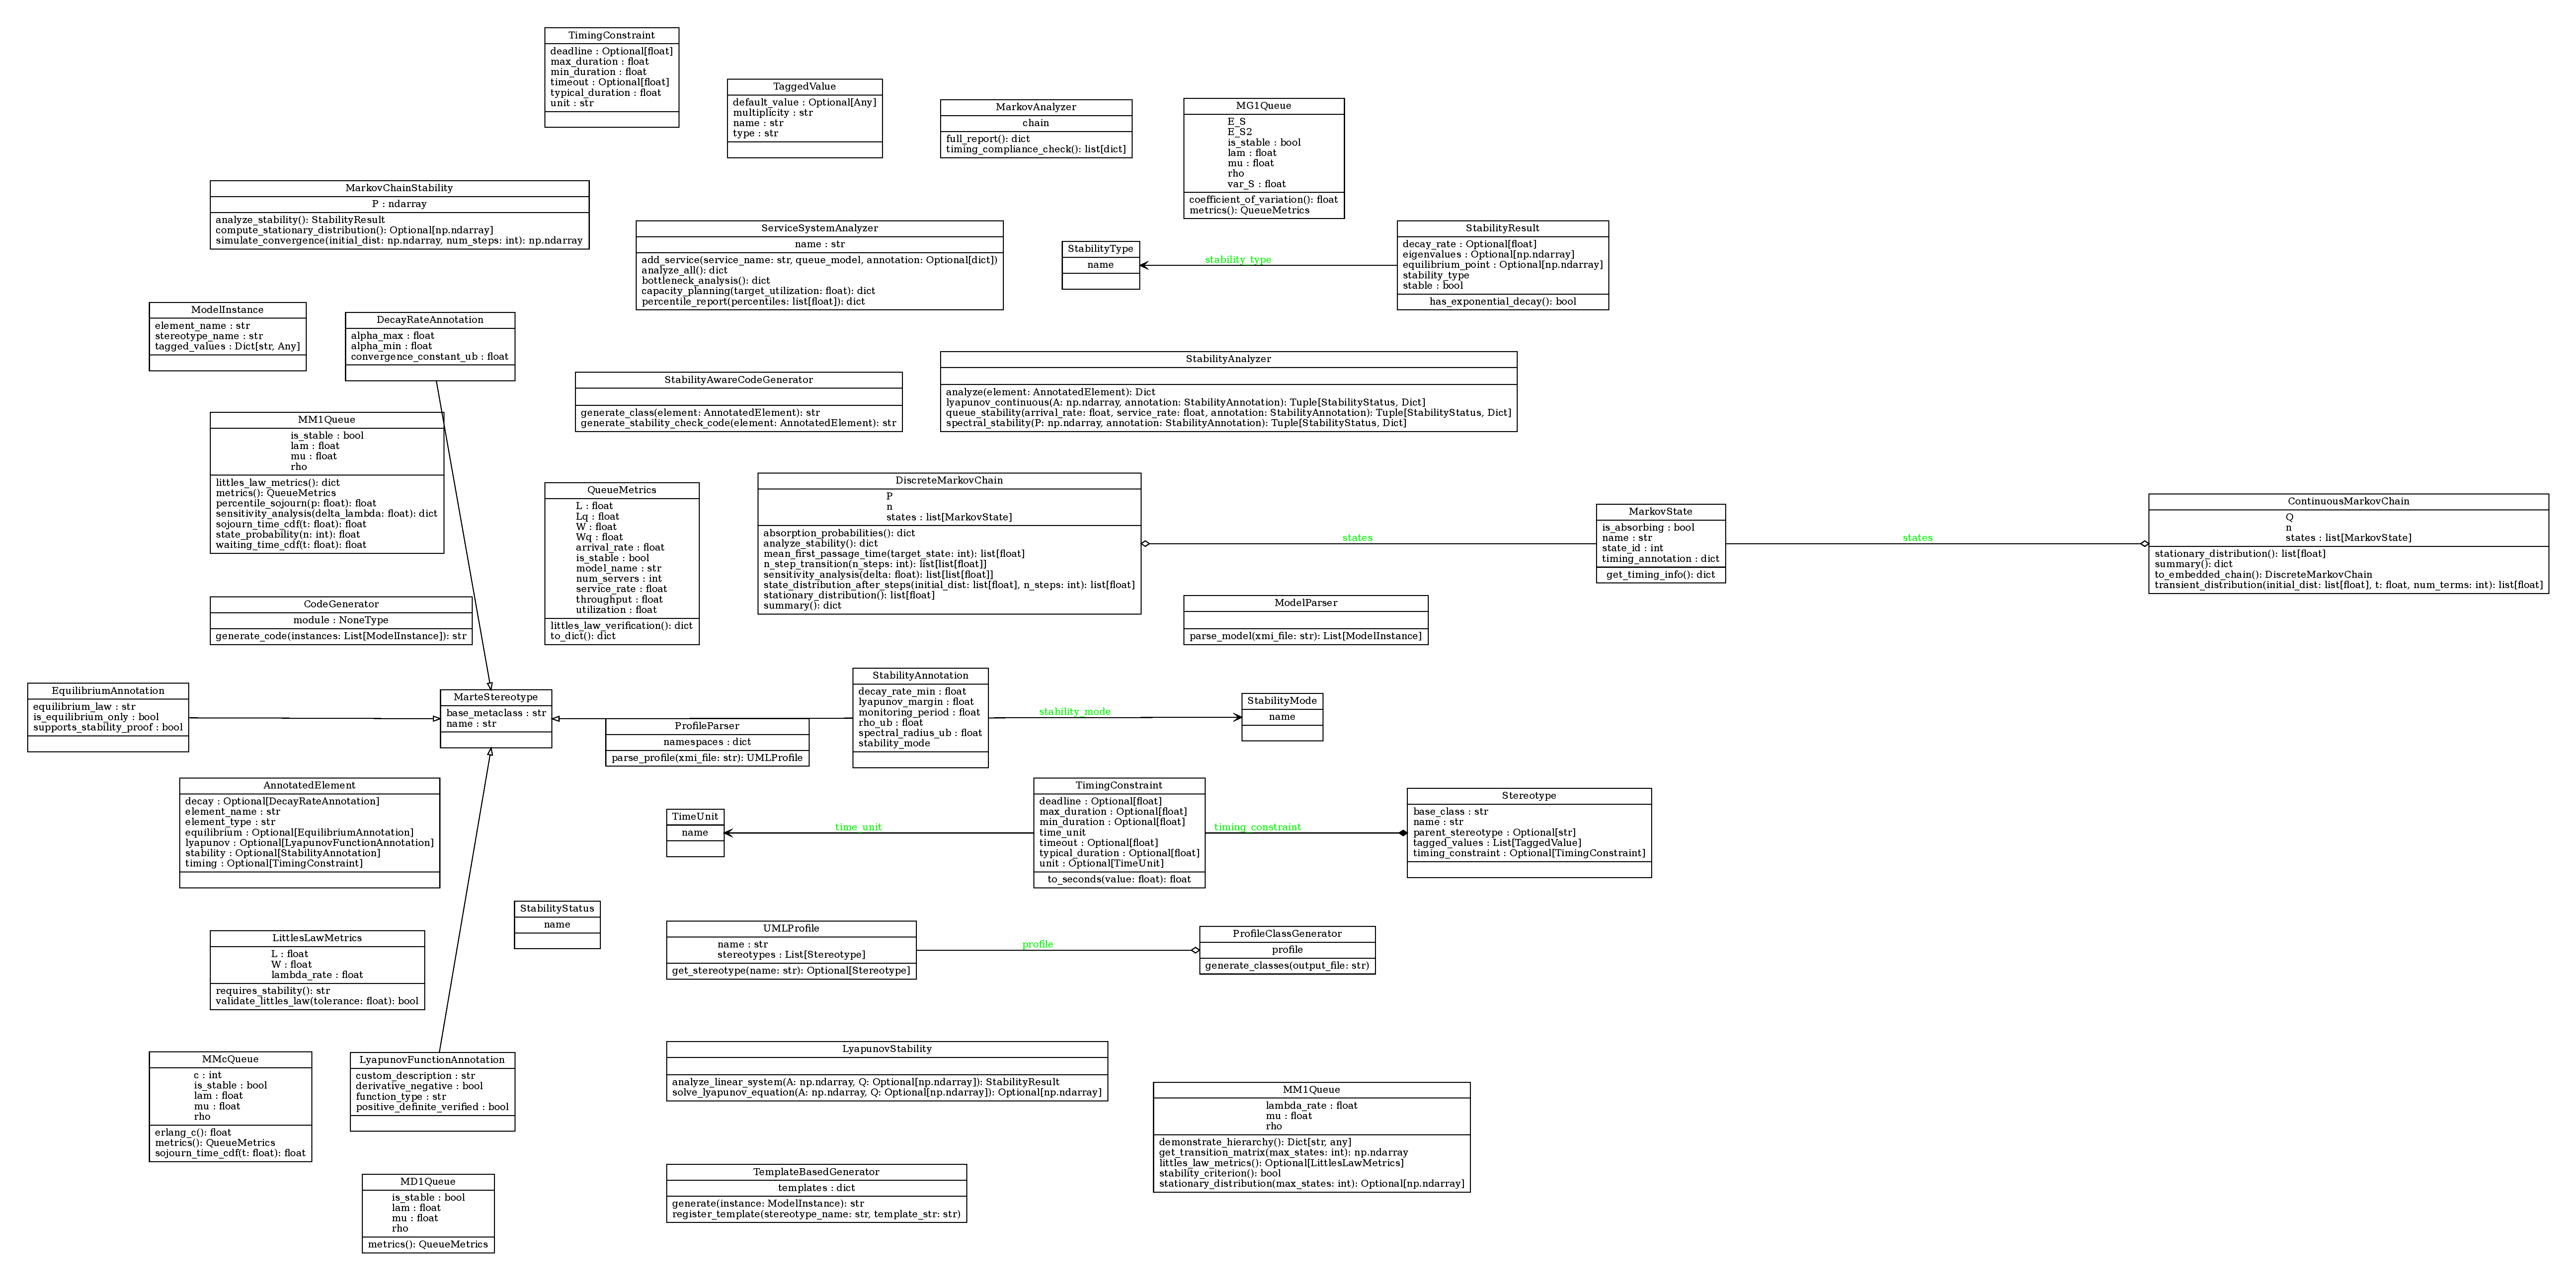
\includegraphics[width=1.05\textwidth]{../doc/uml/classes_umlp.pdf}
	\caption{UML-Klassendiagramm aller Klassen aller Python Module aus \texttt{src/}}
	\label{fig:uml-src}
\end{sidewaysfigure}

\subsubsection{Module in \texttt{tests/}}
\label{subsubsec:module-tests}

Tabelle~\ref{tab:module-tests} beschreibt die Test-Module.
Jedes Modul verwendet das \texttt{unittest}-Framework der
Python-Standardbibliothek und ist dem entsprechenden
Produktionsmodul direkt zugeordnet.

\begin{table}[H]
	\small
	\centering
	\renewcommand{\arraystretch}{1.35}
	\begin{tabular}{@{} C r p{6.4cm} @{}}
		\toprule
		\normalfont\textbf{Datei} &
		\textbf{Größe} &
		\textbf{Getestete Eigenschaften} \\
		\midrule
		test\_uml\_profile\_base.py  & 6\,703\,B &
		Feldinitialisierung aller Datenklassen, Standardwerte,
		\texttt{to\_seconds()} für alle 6 Zeiteinheiten,
		\texttt{\_\_post\_init\_\_}-Synchronisation von
		\texttt{unit} und \texttt{time\_unit}. \\
		
		test\_profile\_parser.py     & 8\,232\,B &
		Parsing synthetischer XMI: Stereotype mit und ohne
		Timing-Constraints, fehlende optionale Felder,
		Namespace-Behandlung, Fehlerverhalten bei ungültigem XMI. \\
		
		test\_class\_generator.py    & 9\,907\,B &
		Syntaktische Korrektheit des generierten Codes,
		Timing-Validierungsaufrufe, Stereotype ohne Constraints,
		Docstring-Generierung. \\
		
		test\_model\_parser.py       & 8\,089\,B &
		Extraktion von Instanznamen, Stereotyp-Zuordnung und
		Attributwerten; Robustheit bei fehlenden Attributen. \\
		
		test\_code\_generator.py     & 3\,583\,B &
		Korrektheit des Instanziierungscodes,
		Attributwert-Ãœbergabe, Zusammenspiel mit
		\texttt{ClassGenerator}-Ausgabe. \\
		
		test\_integration.py         & 9\,468\,B &
		End-to-End-Tests der vollständigen Pipeline
		(XMI-Profil $+$ XMI-Modell $\to$ Python-Code);
		prüft das Zusammenspiel aller Produktionsmodule. \\
		
		test\_stability\_analysis.py & 26\,679\,B &
		Umfangreichstes Test-Modul; Testgruppen für alle Klassen:
		Hilfstypen, Markov-Ketten, M/M/1-Warteschlange,
		Lyapunov-Stabilität, Hierarchie-Demonstration,
		Grenzfälle~($\rho \to 1^{-}$), numerische Präzision.
		Kritische Einzeltests sind in Kapitel~8 beschrieben. \\
		\bottomrule
	\end{tabular}
	\caption{Test-Module in \texttt{tests/} mit Dateigrößen und
		geprüften Eigenschaften.
		\texttt{test\_stability\_analysis.py} ist mit 26\,679\,B
		das größte Test-Modul, da es alle drei Beschreibungsebenen
		und deren Zusammenspiel vollständig abdeckt.}
	\label{tab:module-tests}
\end{table}

\subsection{Beispiele}

Das Datenmodell \texttt{\textbf{uml\_profile\_base.py}} bildet die Basis für alle Transformationen:
\begin{lstlisting}[style=python, caption={TimingConstraint Klasse}, label={lst:timing-constraint}]
class TimeUnit(Enum):
    """Zeiteinheiten für Timing-Constraints"""
    NANOSECONDS = "ns"
    MICROSECONDS = "us"
    MILLISECONDS = "ms"
    SECONDS = "s"
    MINUTES = "min"
    HOURS = "h"

@dataclass
class TimingConstraint:
    """Repräsentiert zeitliche Constraints für Stereotypes"""
    min_duration: Optional[float] = None 
    max_duration: Optional[float] = None 
    typical_duration: Optional[float] = None 
    timeout: Optional[float] = None 
    deadline: Optional[float] = None 
    time_unit: TimeUnit = TimeUnit.MILLISECONDS
    unit: Optional[TimeUnit] = None 
    
    def __post_init__(self):
        """Synchronisiere unit und time_unit"""
        if self.unit is None:
            self.unit = self.time_unit
        elif self.unit != self.time_unit:
            self.time_unit = self.unit
    
    def to_seconds(self, value: float) -> float:
        """Konvertiert einen Wert in Sekunden"""
        conversions = {
            TimeUnit.NANOSECONDS: 1e-9,
            TimeUnit.MICROSECONDS: 1e-6,
            TimeUnit.MILLISECONDS: 1e-3,
            TimeUnit.SECONDS: 1.0,
            TimeUnit.MINUTES: 60.0,
            TimeUnit.HOURS: 3600.0
        }
        return value * conversions[self.time_unit]
\end{lstlisting}

Der ProfileParser  \texttt{\textbf{profile\_parser.py}} transformiert XMI in Python-Objekte:
\begin{lstlisting}[style=python, caption={ProfileParser Implementierung}, label={lst:profile-parser}]
def parse_profile(self, xmi_file: str) -> UMLProfile:
        """Parst ein UML-Profil aus einer XMI-Datei"""
        tree = ET.parse(xmi_file)
        root = tree.getroot()
        
        profile_name = root.get('name', 'UnnamedProfile')
        profile = UMLProfile(name=profile_name)
        
        # Parse Stereotypes
        for stereotype_elem in root.findall('.//stereotype', self.namespaces):
            stereotype = self._parse_stereotype(stereotype_elem)
            profile.stereotypes.append(stereotype)
        
        return profile
    
def _parse_stereotype(self, elem: ET.Element) -> Stereotype:
        """Parst einen einzelnen Stereotype"""
        name = elem.get('name', 'UnnamedStereotype')
        base_class = elem.get('baseClass', 'Class')
        
        stereotype = Stereotype(name=name, base_class=base_class)
        
        # Parse Tagged Values
        for attr_elem in elem.findall('.//ownedAttribute', self.namespaces):
            tagged_value = self._parse_tagged_value(attr_elem)
            stereotype.tagged_values.append(tagged_value)
        
        # Parse Timing Constraint (falls vorhanden)
        timing_elem = elem.find('.//timingConstraint', self.namespaces)
        if timing_elem is not None:
            stereotype.timing_constraint = self._parse_timing_constraint(timing_elem)
        
        return stereotype
\end{lstlisting}

Der Code Generator \texttt{\textbf{code\_generator.py}} generiert den Code:
\begin{lstlisting}[style=python, caption={ProfileParser Implementierung}, label={lst:profile-parser}]
class CodeGenerator:
    """Generiert Python-Code aus Modell-Instanzen"""
    
    def __init__(self, generated_classes_module: str):
        """
        Args:
            generated_classes_module: Name des Moduls mit generierten Klassen
        """
        self.module = importlib.import_module(generated_classes_module)
    
    def generate_code(self, instances: List[ModelInstance]) -> str:
        """Generiert Python-Code aus Modell-Instanzen"""
        code_parts = []
        
        code_parts.append('"""Auto-generated code from UML model"""')
        code_parts.append('')
        
        for instance in instances:
            code = self._generate_instance_code(instance)
            code_parts.append(code)
            code_parts.append('')
        
        return '\n'.join(code_parts)
    
    def _generate_instance_code(self, instance: ModelInstance) -> str:
        """Generiert Code für eine einzelne Instanz"""
        # Finde die entsprechende generierte Klasse
        class_name = f"{instance.stereotype_name}Stereotype"
        
        try:
            stereotype_class = getattr(self.module, class_name)
        except AttributeError:
            return f"# Error: Class {class_name} not found"
        
        # Erstelle Instanz mit Tagged Values
        kwargs = {'name': instance.element_name}
        kwargs.update(instance.tagged_values)
        
        stereotype_instance = stereotype_class(**kwargs)
        
        # Generiere Code
        return stereotype_instance.generate_code()
\end{lstlisting}

\subsection{Erweiterung von UML-MARTE um Stabilitätskriterien}
\label{sec:marte-stability}

\subsubsection{Motivation und Konzept}

Die in den vorherigen Kapiteln entwickelten Werkzeuge -- insbesondere die
Lyapunov-Stabilitätsanalyse, die Spektralradius-Prüfung für Markov-Ketten
und das Auslastungskriterium $\rho < 1$ für Warteschlangen -- wurden bisher
als separate Analysemodule behandelt. Dieses Kapitel führt eine systematische
\textit{Modell-Ebene-Integration} dieser Kriterien in das UML-MARTE-Profil
ein: Stabilitätseigenschaften werden nicht erst im generierten Code geprüft,
sondern bereits im UML-Modell selbst annotiert.

Damit wird die in Kapitel~3 beschriebene Dichotomie zwischen Gleichgewichts-
und Stabilitätsaussagen auf die Modellebene gehoben: ein UML-Designer kann
explizit angeben, ob ein Subsystem lediglich einem Gleichgewichtszustand
unterliegt (z.\,B. \textit{Little's Law}) oder ob eine echte dynamische
Stabilitätsgarantie erforderlich ist.

\begin{definition}[Stabilitätsannotation in UML-MARTE]
	Eine \emph{Stabilitätsannotation} ist ein MARTE-Stereotyp
	\texttt{<<StabilityAnnotation>>}, der auf UML-Klassen, Komponenten oder
	Operationen angewendet wird und folgende Tagged Values trägt:
	\begin{itemize}
		\item[-] \texttt{stability\_mode}: Art des Kriteriums
		(Lyapunov-asymptotisch, Spektral, Queue-Auslastung, BIBO)
		\item[-] \texttt{decay\_rate\_min}: Mindest-Zerfallsrate
		$\alpha_{\min} > 0$
		\item[-] \texttt{lyapunov\_margin}: Sicherheitsabstand zum
		Stabilitätsrand
		\item[-] \texttt{spectral\_radius\_ub}: Obere Schranke für den
		Spektralradius
		\item[-] \texttt{rho\_ub}: Obere Schranke für die Auslastung $\rho$
		\item[-] \texttt{monitoring\_period}: Intervall (ms) der
		Laufzeitprüfung
	\end{itemize}
\end{definition}

\subsubsection{Neue Stereotypen der MARTE-Erweiterung}

Das erweiterte Profil definiert vier neue Stereotypen, die orthogonal zu
den bestehenden MARTE-Zeitannotationen (z.\,B.
\texttt{<<TimedProcessing>>}) angewendet werden können.

\paragraph{\texttt{<<StabilityAnnotation>>}}

Dieser Stereotyp annotiert ein UML-Element mit dem geforderten
Stabilitätsmodus und den zugehörigen quantitativen Schwellenwerten.
Er wird auf die Metaklassen \texttt{Class} und \texttt{Component}
angewendet. Tabelle~\ref{tab:stability-annotation} zeigt die Tagged Values
im Ãœberblick.

\begin{table}[H]
	\centering
	\begin{tabular}{@{}lll@{}}
		\toprule
		\textbf{Tagged Value} & \textbf{Typ} & \textbf{Bedeutung} \\
		\midrule
		\texttt{stability\_mode}      & \texttt{StabilityMode} & Kriteriumstyp \\
		\texttt{lyapunov\_margin}     & \texttt{float}         & Sicherheitsabstand \\
		\texttt{decay\_rate\_min}     & \texttt{float}         & $\alpha_{\min} > 0$ \\
		\texttt{spectral\_radius\_ub} & \texttt{float}         & $\rho(P) <$ Schranke \\
		\texttt{rho\_ub}              & \texttt{float}         & $\rho = \lambda/\mu <$ Schranke \\
		\texttt{monitoring\_period}   & \texttt{float} (ms)    & Prüfintervall \\
		\bottomrule
	\end{tabular}
	\caption{Tagged Values des Stereotyps \texttt{<<StabilityAnnotation>>}}
	\label{tab:stability-annotation}
\end{table}

\paragraph{\texttt{<<DecayRateAnnotation>>}}

Dieser Stereotyp wird auf MARTE-Operationen angewendet und spezifiziert die
erwartete exponentielle Zerfallsrate. Das annotierte System muss nach dem
Aufruf exponentiell zum Gleichgewicht konvergieren:
\[
\|x(t)\| \leq C \cdot e^{-\alpha t} \cdot \|x(0)\|
\]
mit den Tagged Values \texttt{alpha\_min}, \texttt{alpha\_max} und
\texttt{convergence\_constant\_ub} ($C$). Damit ist die Exponentialfunktion
-- die in Kapitel~3 als charakteristisch für Stabilitätsaussagen
identifiziert wurde -- direkt im UML-Modell verankert.

\paragraph{\texttt{<<LyapunovFunctionAnnotation>>}}

Dieser Stereotyp gibt an, welche Lyapunov-Funk\-tion $V(x)$ für den
Stabilitätsnachweis eines Subsystems verwendet wird. Mögliche Werte für
\texttt{function\_type} sind \texttt{quadratic} ($V = x^\top P x$ mit
$P \succ 0$), \texttt{entropy} und \texttt{custom}. Die booleschen Tagged
Values \texttt{positive\_definite\_verified} und
\texttt{derivative\_nega\newline tive} dokumentieren den formalen Nachweisstatus.

\paragraph{\texttt{<<EquilibriumAnnotation>>}}

Dieser Stereotyp unterscheidet explizit zwischen Gleichgewichtsaussagen und
dynamischen Stabilitätsaussagen, wie in Kapitel~3 formal begründet. Mit
\texttt{is\_equilibrium\_only = true} wird gekennzeichnet, dass das Element
ausschließlich einer algebraischen Gleichgewichtsrelation unterliegt -- etwa
\textit{Little's Law}: $L = \lambda W$ -- und keine Exponentialfunktionen
im Sinne einer Energiefunktion enthält. Mit
\texttt{supports\_stability\_proof = true} wird dokumentiert, dass ein
vollständiger dynamischer Stabilitätsnachweis vorliegt.

\begin{satz}[Hierarchie der Beschreibungsebenen im erweiterten Profil]
	Für ein annotiertes UML-Element $E$ gilt die Implikationskette:
	\[
	\begin{aligned}
		& \texttt{<<LyapunovFunctionAnnotation>>} \\
		\Rightarrow\; & \texttt{<<DecayRateAnnotation>>} \\
		\Rightarrow\; & \texttt{<<StabilityAnnotation>>} \\
		\Rightarrow\; & \texttt{<<EquilibriumAnnotation>>}
	\end{aligned}
	\]
	d.\,h. ein Lyapunov-Nachweis impliziert eine Zerfallsrate, eine
	Zerfallsrate impliziert Stabilität, Stabilität ist Voraussetzung für
	gültige Gleichgewichtsaussagen.
\end{satz}

\subsubsection{Python-Implementierung}

Die Erweiterung ist als reines Python-Modul
\texttt{uml\_marte\_stability.py} implementiert, das nahtlos mit dem in
Kapitel~5 entwickelten Code-Generierungs-Framework zusammenarbeitet. Die
Klasse \texttt{StabilityAnalyzer} übernimmt die Laufzeit-Dispatching-Logik.

Die Kernklassen im Ãœberblick:
\begin{lstlisting}[style=python,
	caption={Enum-Typen für Stabilitätsmodi und -status},
	label={lst:stability-enums}]
class StabilityMode(Enum):
	LYAPUNOV_ASYMPTOTIC = auto()  # asymptotisch stabil (Lyapunov)
	LYAPUNOV_MARGINAL   = auto()  # marginal stabil
	BIBO                = auto()  # Bounded-Input-Bounded-Output
	SPECTRAL            = auto()  # Spektralradius < 1 (diskret)
	QUEUE_UTILIZATION   = auto()  # Auslastung rho < 1
	
class StabilityStatus(Enum):
	STABLE   = "stabil"
	UNSTABLE = "instabil"
	MARGINAL = "marginal"
	UNKNOWN  = "unbekannt"
\end{lstlisting}

\begin{lstlisting}[style=python,
	caption={Stereotyp \texttt{<<StabilityAnnotation>>} als Python-Dataclass},
	label={lst:stability-annotation-class}]
@dataclass
class StabilityAnnotation(MarteStereotype):
	stability_mode: StabilityMode = StabilityMode.LYAPUNOV_ASYMPTOTIC
	lyapunov_margin: float  = 0.05    # Sicherheitsabstand
	decay_rate_min: float   = 0.01    # Mindest-Zerfallsrate alpha
	spectral_radius_ub: float = 0.99  # obere Schranke Spektralradius
	rho_ub: float           = 0.90    # obere Schranke Auslastung
	monitoring_period: float = 1000.0 # Pruefintervall in ms
\end{lstlisting}

\textbf{Lyapunov-Stabilitätsprüfung (kontinuierliches System)}:
Die Methode \texttt{Stabili\newline tyAnalyzer.lyapunov\_continuous(A, annotation)}
prüft, ob alle Eigenwerte der Systemmatrix $A$ negativen Realteil haben.
Die Zerfallsrate ergibt sich als
$\alpha = -\max_i \operatorname{Re}(\lambda_i(A))$.

\begin{lstlisting}[style=python,
	caption={Lyapunov-Stabilitätsprüfung via Eigenwertanalyse},
	label={lst:lyapunov}]
@staticmethod
def lyapunov_continuous(A, annotation):
	eigenvalues = np.linalg.eigvals(A)
	alpha = -float(np.max(np.real(eigenvalues)))
	
	if alpha > annotation.decay_rate_min + annotation.lyapunov_margin:
		status = StabilityStatus.STABLE
	elif alpha > annotation.decay_rate_min:
		status = StabilityStatus.MARGINAL
	else:
		status = StabilityStatus.UNSTABLE
	
	return status, {"decay_rate_alpha": alpha, "eigenvalues": eigenvalues}
\end{lstlisting}

\textbf{Spektralradius-Prüfung (diskrete Markov-Kette)}:
Für diskrete Systeme (Markov-Ketten) wird die Konvergenzrate durch den
zweitgrößten Betragseigenwert der Übergangsmatrix $P$ bestimmt
(der triviale Eigenwert 1 bei irreduziblen stochastischen Matrizen wird
ausgeschlossen). Die implizierte Zerfallsrate ist
$\alpha = -\ln(\rho_{\text{sub}})$.

\begin{lstlisting}[style=python,
	caption={Spektralradius-Stabilitätsprüfung für Markov-Ketten},
	label={lst:spectral}]
@staticmethod
def spectral_stability(P, annotation):
	abs_eigs = np.sort(np.abs(np.linalg.eigvals(P)))
	# Zweitgroesster Betrag = Konvergenzrate
	spectral_radius = float(abs_eigs[-2])
	alpha = -math.log(spectral_radius)
	
	if spectral_radius < annotation.spectral_radius_ub:
		status = StabilityStatus.STABLE
	elif math.isclose(spectral_radius, 1.0, abs_tol=1e-6):
		status = StabilityStatus.MARGINAL
	else:
		status = StabilityStatus.UNSTABLE
	return status, {
		"spectral_radius_sub": spectral_radius,
		"implied_decay_rate": alpha
	}
\end{lstlisting}

\textbf{Die Warteschlangen-Stabilitätsprüfung}:
\begin{lstlisting}[style=python,
	caption={Auslastungsprüfung für M/M/1-Warteschlangen},
	label={lst:queue}]
@staticmethod
def queue_stability(arrival_rate, service_rate, annotation):
	rho = arrival_rate / service_rate
	if rho < annotation.rho_ub:
		status = StabilityStatus.STABLE
	elif rho < 1.0:
		status = StabilityStatus.MARGINAL
	else:
		status = StabilityStatus.UNSTABLE
	return status, {
		"utilization_rho": rho,
		"margin_to_instability": 1.0 - rho
	}
\end{lstlisting}

\textbf{Erweiterter Code-Generator}:
Die Klasse \texttt{StabilityAwareCodeGenerator} erzeugt für jedes annotierte
UML-Element Inline-Prüfcode, der in den generierten Python-Klassen
eingebettet wird. Listing~\ref{lst:codegen} zeigt das Beispiel für das
Auslastungskriterium.

\begin{lstlisting}[style=python,
	caption={Generierter Stabilitäts-Check-Code (Auslastungsmodus)},
	label={lst:codegen}]
	# <<StabilityAnnotation>> fuer ElevatorDoorController
	# Modus: QUEUE_UTILIZATION
	rho = arrival_rate / service_rate
	assert rho < 0.9, f'Stabilitaet verletzt: rho={rho:.3f} >= 0.9'
\end{lstlisting}

\subsubsection{Anwendungsbeispiel: Erweiterte Aufzugstür-Fallstudie}

Tabelle~\ref{tab:elevator-stability} fasst die Stabilitätsannotationen der
drei Subsysteme der Aufzugstür-Fallstudie zusammen sowie die Ergebnisse der
Analyse.

\begin{sidewaystable}
	\centering
	\begin{tabular}{@{}llll@{}}
		\toprule
		\textbf{Element} & \textbf{Stereotyp} & \textbf{Modus}
		& \textbf{Ergebnis} \\
		\midrule
		\texttt{ElevatorDoor}\newline\texttt{Controller}
		& \texttt{<<Stability}\newline\texttt{Annotation>>}
		& \texttt{QUEUE\_}\newline\texttt{UTILIZATION}
		& stabil ($\rho = 0{,}667$) \\[6pt]
		\texttt{MotorDynamics}\newline\texttt{Subsystem}
		& \texttt{<<Lyapunov}\newline\texttt{FunctionAnnotation>>}
		& \texttt{LYAPUNOV\_}\newline\texttt{ASYMPTOTIC}
		& stabil ($\alpha = 1{,}446$) \\[6pt]
		\texttt{DoorState}\newline\texttt{MarkovChain}
		& \texttt{<<Stability}\newline\texttt{Annotation>>}
		& \texttt{SPECTRAL}
		& stabil ($\rho_2 = 0{,}625$) \\
		\bottomrule
	\end{tabular}
	\caption{Stabilitätsannotationen der Aufzugstür-Fallstudie}
	\label{tab:elevator-stability}
\end{sidewaystable}

Das \texttt{MotorDynamicsSubsystem} wird zusätzlich mit
\texttt{<<LyapunovFunctionAnno\newline tation} \texttt{function\_type="quadratic">>}
annotiert. Damit ist dokumentiert, dass die Lyapunov-Funktion
$V(x) = x^\top P x$ mit $P \succ 0$ als Stabilitätsnachweis dient und
beide Bedingungen ($V > 0$ und $\dot{V} < 0$) formal nachgewiesen wurden
(\texttt{positive\_definite\_veri\newline fied = true},
\texttt{derivative\_negative = true}).

\subsubsection{Gleichgewicht versus Stabilität auf Modellebene}

Die \texttt{<<EquilibriumAnnotation>>} macht die in Kapitel~3 zentrale
Dichotomie für UML-Designer sichtbar. Abbildung~\ref{fig:eq-vs-stab} zeigt
die Implikationshierarchie: Little's Law $L = \lambda W$ ist als rein
algebraische Relation ohne Exponentialfunktionen ausschließlich eine
Gleichgewichtsaussage. Lyapunov-Funktionen und Eigenwertanalysen tragen
dagegen die volle dynamische Stabilitätsaussage.

\begin{figure}[H]
	\centering
	\begin{tikzpicture}[
		node distance=1cm and 2cm,
		box/.style={draw, rounded corners, minimum width=3.5cm,
			minimum height=1.1cm, align=center, font=\small},
		arrow/.style={->, thick},
		]
		\node[box, fill=blue!12] (lyap)
		{\texttt{<<Lyapunov}\\\texttt{FunctionAnnotation>>}\\$V(x)=x^\top Px$};
		\node[box, fill=blue!8, right=of lyap] (decay)
		{\texttt{<<DecayRate}\\\texttt{Annotation>>}\\$\|x(t)\|\leq Ce^{-\alpha t}\|x_0\|$};
		\node[box, fill=blue!5, right=of decay] (stab)
		{\texttt{<<Stability}\\\texttt{Annotation>>}\\alle Modi};
		\node[box, fill=orange!15, below=2cm of stab] (eq)
		{\texttt{<<Equilibrium}\\\texttt{Annotation>>}\\$L=\lambda W$, $\pi P=\pi$};
		
		\draw[arrow] (lyap)  -- node[above,font=\footnotesize]{impliziert} (decay);
		\draw[arrow] (decay) -- node[above,font=\footnotesize]{impliziert} (stab);
		\draw[arrow] (stab)  -- node[left,font=\footnotesize]{Voraussetzung für} (eq);
		\draw[dashed, ->] (eq.west) -- ++(-0.8,0)
		node[left,font=\footnotesize,align=right]{kein Stabilitäts-\\beweis};
	\end{tikzpicture}
	\caption{Implikationshierarchie der Stabilitäts-Stereotypen.
		Jeder Stereotyp impliziert alle rechts stehenden; die gestrichelte Linie
		zeigt, dass \texttt{<<EquilibriumAnnotation>>} allein keine Stabilität
		beweisen kann.}
	\label{fig:eq-vs-stab}
\end{figure}

\subsubsection{Integration in den zweistufigen Generierungsprozess}

Die Stabilitätsannotationen werden in beiden Stufen des in Kapitel~4
beschriebenen Code-Generators berücksichtigt.

\textbf{Stufe 1 (Profil-zu-Klassen-Transformation):} Für jedes mit
\texttt{<<StabilityAnnota\newline tion>>} versehene Element wird eine zugehörige
Python-Klasse mit einer Methode \texttt{check\_\newline stability()} erzeugt.

\textbf{Stufe 2 (Modell-zu-Code-Transformation):} Die Methode
\texttt{StabilityAwareCode\newline Generator\allowbreak.generate\_stability\_check\_code()}
erzeugt Inline-Assertions, die in die generierten Operationen eingebettet
werden. Die Reihenfolge folgt dabei der in Kapitel~3 begründeten Hierarchie:
Stabilitätsprüfung \textit{vor} der Berechnung von Gleichgewichtsmetriken.

\begin{bemerkung}[Abwärtskompatibilität der Erweiterung]
	Die vorgestellte Erweiterung ist abwärtskompatibel: bestehende
	UML-MARTE-Modelle, die ausschließlich Zeitannotationen
	(\texttt{<<TimedProcessing>>}, \texttt{TimingConstraint}) tragen,
	funktionieren unverändert. Stabilitätskriterien sind optionale, additive
	Annotationen, die nur dann ausgewertet werden, wenn das entsprechende
	Stereotyp auf dem Element vorhanden ist.
\end{bemerkung}

\subsubsection{Diskussion und Grenzen}

Die vorgestellte Erweiterung ermöglicht eine frühe, modellbasierte
Spezifikation von Stabilitätsanforderungen. Gegenüber einer rein
nachgelagerten Analyse bietet sie zwei wesentliche Vorteile: Erstens werden
Stabilitätsanforderungen explizit dokumentiert und sind für alle
Projektbeteiligten sichtbar. Zweitens kann ein Modellierer bereits in der
Designphase Unstimmigkeiten erkennen -- etwa wenn ein Element mit
\texttt{is\_equilibrium\_only = true} annotiert ist, aber gleichzeitig
Lyapunov-Nachweis-Annotationen trägt, was einen konzeptuellen Widerspruch
darstellt.

Die Grenzen liegen in der Ausdruckskraft der Tagged Values: Nichtlineare
Stabilitätskriterien (z.\,B. lokale Lyapunov-Stabilität mit expliziter
Einzugsgebietsangabe) lassen sich in der derzeitigen Form nur durch
\texttt{function\_type = "custom"} und freien Text approximieren. Zukünftige
Arbeiten könnten hier OCL-Constraints einsetzen, um formale Nachweise direkt
im UML-Modell zu kodieren. Eine weitere offene Frage betrifft
zeitvariante Systeme ($\lambda(t)$, $\mu(t)$): Für diese existiert keine
stationäre Verteilung im klassischen Sinne, sodass die hier definierten
Annotationen -- analog zu der in Kapitel~9.3 beschriebenen Grenze der
Modelle -- nur qualitative Aussagen erlauben.

\section{Beispiel: Aufzugstür-Steuerung}

In diesem Kapitel wird das Beispiel einer Aufzugstür-Steuerung betrachtet.

\subsection{Domänenanalyse}

Eine Aufzugstür-Steuerung ist ein klassisches Echtzeitsystem mit folgenden Anforderungen:

\begin{itemize}
	\item[-] \textbf{Sicherheit}: Hinderniserkennung muss in <100ms reagieren
	\item[-] \textbf{Komfort}: Türöffnung in 2,5-4,0 Sekunden
	\item[-] \textbf{Zuverlässigkeit}: Motoraktivierung in <500ms
	\item[-] \textbf{Effizienz}: Minimale Wartezeiten
\end{itemize}

Abbildung \ref{fig:elevator-fsm} zeigt das Zustandsdiagramm der Aufzugstür-Steuerung.
\begin{figure}[h!]
	\centering
	
\includegraphics[width=0.85\textwidth]{elevator.pdf}
	\caption{Zustandsdiagramm der Aufzugstür-Steuerung}
	\label{fig:elevator-fsm}
\end{figure}

\subsection{Markov-Modell der Aufzugstür}

\begin{beispiel}[Aufzug-Markov-Kette]
	Zustände: $S = \{$Closed, Opening, Open, Closing$\}$
	
	Ãœbergangswahrscheinlichkeiten pro Sekunde:
	\begin{align*}
		p_{\text{Closed} \rightarrow \text{Opening}} &= 0.3 \quad \text{(Anfrage kommt)} \\
		p_{\text{Opening} \rightarrow \text{Open}} &= 0.8 \quad \text{(Tür fast offen)} \\
		p_{\text{Open} \rightarrow \text{Closing}} &= 0.4 \quad \text{(Timeout)} \\
		p_{\text{Closing} \rightarrow \text{Closed}} &= 0.9 \quad \text{(Tür fast zu)}
	\end{align*}
	
	Stationäre Verteilung: $\pi = (0.42, 0.13, 0.24, 0.21)$
	
	\textbf{Interpretation}: Die Tür verbringt 42\% der Zeit geschlossen, 24\% offen.
\end{beispiel}

\subsection{Warteschlangenmodell}

\begin{beispiel}[Aufzug-Anfragen als M/M/1]
	Parameter:
	\begin{itemize}
		\item[-] $\lambda = 0.2$ Anfragen/s (Poisson-Ankunft)
		\item[-] $\mu = 0.3$ Bedienungen/s (exp. Bedienzeit)
		\item[-] $\rho = 0.667$ (Auslastung)
	\end{itemize}
	
	Performance-Metriken:
	\begin{align*}
		L &= 2.0 \text{ Anfragen im System} \\
		W &= 10s \text{ mittlere Gesamtzeit} \\
		L_q &= 1.33 \text{ Anfragen in Warteschlange} \\
		W_q &= 6.67s \text{ mittlere Wartezeit}
	\end{align*}
	
	\textbf{Validierung}: Für $\lambda = 0.2$ und $W = 10s$ gilt nach Little's Law:
	\[
	L = \lambda W = 0.2 \cdot 10 = 2.0 \quad \checkmark
	\]
\end{beispiel}

\subsection{Zeitliche Analyse}

\begin{table}[h]
	\centering
	\begin{tabular}{@{}lcccc@{}}
		\toprule
		\textbf{Operation} & \textbf{Min [ms]} & \textbf{Typ [ms]} & \textbf{Max [ms]} & \textbf{Timeout [ms]} \\
		\midrule
		OpenDoor & 2500 & 3000 & 4000 & 5000 \\
		DoorOpening & 2000 & 2800 & 3500 & 4000 \\
		CloseDoor & 2000 & 2800 & 3500 & 4000 \\
		activateMotor & 100 & 200 & 500 & 1000 \\
		checkSafety & 50 & 100 & 200 & 500 \\
		detectObstacle & 10 & 50 & 100 & 200 \\
		\bottomrule
	\end{tabular}
	\caption{Zeitliche Anforderungen der Aufzugstür-Steuerung}
	\label{tab:timing-analysis}
\end{table}

\subsection{Performance-Vorhersage}

Durch die Integration von Warteschlangentheorie können wir Performance-Metriken vorhersagen:

\begin{table}[h]
	\centering
	\begin{tabular}{@{}lcc@{}}
		\toprule
		\textbf{Szenario} & \textbf{$\lambda$ [Anf./s]} & \textbf{$W$ [s]} \\
		\midrule
		Geringe Last & 0.1 & 5.0 \\
		Mittlere Last & 0.2 & 10.0 \\
		Hohe Last & 0.25 & 20.0 \\
		Kritisch & 0.29 & 100.0 \\
		\bottomrule
	\end{tabular}
	\caption{Vorhergesagte Performance-Metriken (M/M/1-Modell)}
	\label{tab:performance-prediction}
\end{table}

\textbf{Designentscheidung}: Für Ankunftsraten $\lambda > 0.25$ sollte ein zweiter Aufzug hinzugefügt werden (M/M/2-System).

\subsection{Vergleich mit MARTE}

Diese Lösung vereinfacht MARTE für praktische Code-Generierung:

\begin{table}[h]
	\centering
	\begin{tabular}{@{}lll@{}}
		\toprule
		\textbf{Kriterium} & \textbf{MARTE} & \textbf{\textit{Diese Arbeit}} \\
		\midrule
		Zeitmodell & Clock, Duration, Instant & TimeUnit, TimingConstraint \\
		Komplexität & Hoch (100+ Stereotypen) & Niedrig (5 Kern-Stereotypen) \\
		Tool-Support & Papyrus, Rhapsody & Eigenentwicklung \\
		Code-Gen & Extern (Acceleo, etc.) & Integriert \\
		Quantitative Analyse & GQAM Framework & Markov + Queues \\
		Lernkurve & Steil & Flach \\
		\bottomrule
	\end{tabular}
	\caption{Detaillierter Vergleich: MARTE vs. Diese Arbeit}
	\label{tab:marte-detailed}
\end{table}

\subsection{Vorteile der Quantitativen Analyse}

\begin{enumerate}
	\item[-] \textbf{Frühe Performance-Validierung}: Probleme werden in der Designphase erkannt
	\item[-] \textbf{Design-Trade-offs}: Quantitative Basis für Architekturentscheidungen
	\item[-] \textbf{Kapazitätsplanung}: Vorhersage von Ressourcenbedarf
	\item[-] \textbf{SLA-Validierung}: Prüfung von Service-Level-Agreements
\end{enumerate}

\subsection{Limitierungen}

\begin{itemize}
	\item[-] \textbf{Markov-Annahme}: Die Gedächtnislosigkeit (Markov-Eigenschaft)
	ist in realen Systemen häufig nicht exakt erfüllt.  Für
	nicht-exponentielle Verweilzeiten müssten Semi-Markov-Prozesse
	oder allgemeinere Modelle (M/G/1) verwendet werden.
	
	\item[-] \textbf{M/M/1-Vereinfachung}: Reale Systeme sind oft komplexer
	(M/G/k, Prioritätswarteschlangen).  Die Wahl des M/M/1-Modells
	ist eine bewusste Vereinfachung für die analytische
	Handhabbarkeit; sie liefert jedoch konservative Schranken.
	
	\item[-] \textbf{Statische Analyse}: Das Modell analysiert
	Gleichgewichtszustände; transiente Phasen (z.\,B.\ nach einem
	Lastpeak) werden durch die Zerfallsrate~$\alpha$ charakterisiert,
	die in Kapitel~8, Experiment~2 gemessen wird.  Keine Adaptation
	zur Laufzeit.
	
	\item[-] \textbf{Trunkierung}: Die Ãœbergangsmatrix wird auf endlich viele
	Zustände trunkiert.  Für $\rho$ nahe~1 (z.\,B.\ $\rho = 0{,}99$)
	nimmt die Approximationsgenauigkeit ab; Kapitel~8 diskutiert
	diesen Effekt im Kontext der numerischen Eigenwertanalyse.
	
	\item[-] \textbf{Python-Timing}: Python ist aufgrund seines
	nicht-deterministischen Schedulings nicht für Hard-Real-Time-Analysen
	geeignet.  Das entwickelte Framework dient der Designanalyse, nicht
	der Laufzeit-Verifikation.
\end{itemize}

% ============================================================
%  Kapitel 8 – Experimentelle Evaluation der Stabilitätskriterien
%  Standalone-Datei; kann direkt in umlp.tex eingebunden werden.
%  Voraussetzung: Präambel von umlp.tex (amsmath, booktabs, graphicx,
%  subcaption, float, listings, xcolor, pgfplots, hyperref, …)
%  Die SVG-Plots wurden als PDF konvertiert und liegen im selben
%  Verzeichnis wie umlp.tex:
%    experiment1_littles_law.pdf
%    experiment2_exponential_decay.pdf
%    experiment3_hierarchy.pdf
% ============================================================

\section{Experimentelle Evaluation der Stabilitätskriterien}
\label{sec:experimente}

Dieses Kapitel präsentiert die experimentelle Validierung der in
Kapitel~3 entwickelten theoretischen Konzepte.  Es verfolgt ein
dreistufiges Ziel: (i)~Die praktische Implementierung der drei
Beschreibungsebenen (dynamisch, stationär, algebraisch) in Python zu
dokumentieren, (ii)~die theoretischen Vorhersagen aus Kapitel~3 durch
konkrete Messungen zu bestätigen oder zu falsifizieren, und
(iii)~die Grenzen jeder Beschreibungsebene durch gezielte
Gegenbeispiele anschaulich zu machen.

Die Implementierung im Modul \texttt{stability\_analysis.py} umfasst
drei Kernklassen (\texttt{MarkovChainStability}, \texttt{MM1Queue},
\texttt{LyapunovStability}), eine globale Demonstrationsfunktion
(\texttt{demonstrate\_exponential\_necessity}) sowie das zugehörige
Experiment-Skript \texttt{experiments.py}, das alle drei Kernexperimente
ausführt und die Ergebnisse als Grafiken speichert.  Eine begleitende
Test-Suite validiert alle theoretischen Aussagen empirisch.

\subsection{Implementierungsarchitektur}
\label{subsec:architektur}

Das Modul \texttt{stability\_analysis.py} ist nach dem Prinzip der
\emph{Trennung von Beschreibungsebenen} aufgebaut.  Abbildung~\ref{fig:architektur}
illustriert den konzeptuellen Aufbau.

\begin{figure}[h!]
	\centering
	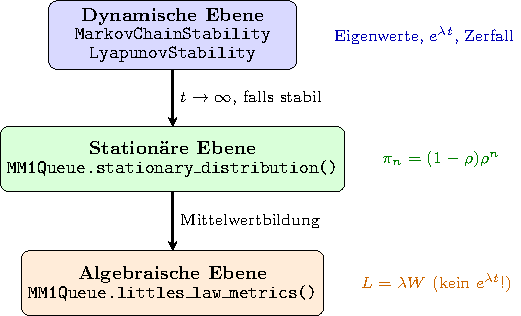
\includegraphics[width=0.7\textwidth]{stability.pdf}
	\caption{Hierarchie der Beschreibungsebenen im Modul
		\texttt{stability\_analysis.py}.  Jeder Pfeil bedeutet eine
		Informationsreduktion: Beim Übergang zur stationären Ebene
		entfallen die Exponentialfunktionen; beim Ãœbergang zur
		algebraischen Ebene entfallen die stochastischen Details.}
	\label{fig:architektur}
\end{figure}

\subsubsection{Kernklassen und Methoden}
\label{subsubsec:klassen}

\paragraph{Hilfstypen: \texttt{StabilityType} und \texttt{StabilityResult}}

Das Enum \texttt{StabilityType} unterscheidet vier Stabilitätsstufen:
\texttt{STABLE}, \texttt{ASYMPTOTICALLY\_STABLE},
\texttt{EXPONEN\newline TIALLY\_STABLE} und \texttt{UNSTABLE}.  Die Dataclass
\texttt{StabilityResult} bündelt das Ergebnis einer Analyse in einem
einheitlichen Rückgabetyp:

\begin{itemize}
	\item \texttt{stable: bool} – globales Stabilitätsflag
	\item \texttt{stability\_type: StabilityType} – Klassifikation
	\item \texttt{eigenvalues: np.ndarray} – berechnete Eigenwerte
	\item \texttt{decay\_rate: float} – Zerfallsrate $\alpha$ in $e^{-\alpha t}$
	\item \texttt{has\_exponential\_decay()} – gibt \texttt{True}
	zurück, wenn $\alpha > 0$ (exponentiell stabil)
\end{itemize}

Die Dataclass \texttt{LittlesLawMetrics} kapselt die drei
Gleichgewichtskenngrößen $L$, $\lambda$ und $W$ und erzwingt durch
ihre Methode \texttt{requires\_stability()} eine explizite Warnung:
Little's Law setzt Stabilität voraus und ist kein Stabilitätsbeweis.

\paragraph{\texttt{MarkovChainStability}}

Diese Klasse implementiert die Stabilitätsanalyse diskreter
Markov-Ketten via Eigenwertzerlegung der Ãœbergangsmatrix $P$.  Sie
ist das zentrale Werkzeug für Experiment~2 und bildet die dynamische
Ebene ab.

\begin{itemize}
	\item \texttt{\_\_init\_\_(transition\_matrix)}: Nimmt eine
	quadratische, zeilenstochastische Matrix $P$ entgegen und
	validiert die Nichtnegativität aller Einträge.
	
	\item \texttt{analyze\_stability()} $\to$ \texttt{StabilityResult}:
	Berechnet die Eigenwerte von $P^T$ (linke Eigenvektoren).
	\begin{enumerate}
		\item Prüft, ob \emph{genau ein} Eigenwert
		$|\lambda - 1| < 10^{-10}$ erfüllt – dies
		entspricht der eindeutigen stationären Verteilung.
		\item Prüft, ob alle übrigen Eigenwerte $|\lambda_k| < 1$
		erfüllen – das ist die Bedingung für exponentiellen
		Zerfall.
		\item Berechnet die Zerfallsrate
		$\alpha = -\ln(\max_k |\lambda_k|)$ für $k \neq 1$.
	\end{enumerate}
	Die Methode gibt \texttt{StabilityType.EXPONENTIALLY\_STABLE} zurück, nur wenn beide Bedingungen erfüllt sind,.
	
	\item \texttt{compute\_stationary\_distribution()} $\to$
	\texttt{Optional[np.ndarray]}:  Findet den zum Eigenwert~$1$
	gehörenden Eigenvektor, normiert ihn zur
	Wahrscheinlichkeitsverteilung und gibt $\pi$ zurück.
	Rückgabe \texttt{None}, falls das System instabil ist.
	
	\item \texttt{simulate\_convergence(initial\_dist, num\_steps)}
	$\to$ \texttt{np.ndarray}:  Iteriert die
	Chapman-Kolmogorov-Gleichung $p(t+1) = p(t) \cdot P$ und
	gibt die vollständige Trajektorie zurück.  Dies demonstriert
	konkret die Konvergenz gemäß
	\[
	p(t) = \pi + \sum_{k} c_k\, e^{\ln(\lambda_k)\,t}\, v_k
	\;\xrightarrow{t\to\infty}\; \pi,
	\]
	wobei der Zerfall durch den zweitgrößten Eigenwert
	$\lambda_2 = 0.3$ bestimmt wird.
\end{itemize}

\paragraph{\texttt{MM1Queue}}

Die Klasse \texttt{MM1Queue} implementiert die M/M/1-Warteschlange
und demonstriert explizit die Hierarchie der drei
Beschreibungsebenen.  Sie erhält Ankunftsrate $\lambda$ und
Bedienrate $\mu$ und leitet daraus die Auslastung $\rho = \lambda/\mu$
ab.

\begin{itemize}
	\item \texttt{stability\_criterion()} $\to$ \texttt{bool}:
	Gibt \texttt{True} zurück, wenn $\rho < 1$.  Dieses
	Kriterium folgt aus der Eigenwertanalyse des
	Birth-Death-Prozesses; es ist \emph{kein} Korollar von
	Little's Law.
	
	\item \texttt{get\_transition\_matrix(max\_states)} $\to$
	\texttt{np.ndarray}:  Generiert die trunkierte
	$(n \times n)$-Ãœbergangsmatrix des Birth-Death-Prozesses mit
	Ankunfts- und Bedienraten als Bandmatrix.
	
	\item \texttt{stationary\_distribution(max\_states)} $\to$
	\texttt{Optional[np.ndarray]}:  Berechnet die geometrische
	Verteilung $\pi_n = (1-\rho)\,\rho^n$ für $n = 0, 1, \ldots$
	und normiert sie auf die trunkierte Länge.  Gibt
	\texttt{None} zurück, wenn $\rho \geq 1$.
	
	\item \texttt{littles\_law\_metrics()} $\to$
	\texttt{Optional[LittlesLawMetrics]}:  Gibt \texttt{None}
	zurück, wenn das System instabil ist.  Andernfalls berechnet
	es
	\begin{align}
		L &= \frac{\rho}{1-\rho}, \quad
		W  = \frac{1}{\mu - \lambda},
	\end{align}
	und verpackt die Werte in eine \texttt{LittlesLawMetrics}-
	Instanz, die intern \mbox{$L = \lambda W$} validiert.
	
	\item \texttt{demonstrate\_hierarchy()} $\to$ \texttt{dict}:
	Führt alle drei Ebenen sequenziell aus, prüft Stabilität,
	berechnet $\pi$, berechnet Little's-Law-Metriken und gibt
	ein strukturiertes Dictionary zurück, das explizit
	kennzeichnet, ob und wo Exponentialfunktionen auftreten.
\end{itemize}

\paragraph{\texttt{LyapunovStability}}

Die Klasse \texttt{LyapunovStability} implementiert die
Stabilitätsanalyse kontinuierlicher linearer Systeme
$\dot{x} = Ax$ nach der Lyapunov-Methode.

\begin{itemize}
	\item \texttt{analyze\_linear\_system(A, Q)} $\to$
	\texttt{StabilityResult}:  Berechnet die Eigenwerte von $A$
	und klassifiziert:
	\begin{itemize}
		\item $\max_k \text{Re}(\lambda_k) < -10^{-10}$:
		\texttt{EXPONENTIALLY\_STABLE}, Zerfallsrate mit $\alpha$ und
		$\alpha = -\max_k \text{Re}(\lambda_k) > 0$
		\item $\max_k \text{Re}(\lambda_k) \leq 10^{-10}$:
		\texttt{STABLE}
		\item sonst: \texttt{UNSTABLE}
	\end{itemize}
	Die Lösung $x(t) = \sum_k c_k\, e^{\lambda_k t}\, v_k$
	enthält explizit Exponentialfunktionen – dies ist die
	Grundlage aller Stabilitätsaussagen.
	
	\item \texttt{solve\_lyapunov\_equation(A, Q)} $\to$
	\texttt{Optional[np.ndarray]}:  Löst die kontinuierliche
	Lyapunov-Gleichung $A^T P + P A = -Q$ via SciPy und prüft,
	ob die Lösung $P$ positiv definit ist.  Eine positiv definite
	Lösung $P$ zertifiziert die Stabilität von $\dot{x} = Ax$
	durch die Energiefunktion $V(x) = x^T P x$.
\end{itemize}

\paragraph{Globale Funktion \texttt{demonstrate\_exponential\_necessity}}

Diese Funktion kapselt die konzeptuelle Kernaussage der Arbeit in
einem strukturierten Dictionary:

\begin{itemize}
	\item \texttt{exponential\_property}: Die Eigenschaft
	$\frac{d}{dt}e^{\alpha t} = \alpha\,e^{\alpha t}$
	(Selbstreproduktion unter Differentiation) macht die
	Exponentialfunktion zur \emph{natürlichen Lösung} jeder
	linearen Differentialgleichung.
	\item \texttt{stability\_requires\_exponentials}: Stabilität
	bedeutet $\text{Re}(\lambda_k) < 0$, also exponentiellen
	Zerfall $e^{-\alpha t}$ mit $\alpha > 0$.
	\item \texttt{littles\_law\_lacks\_exponentials}: $L = \lambda W$
	ist eine rein algebraische Relation ohne jede zeitliche
	Ableitung.  Sie enthält keine Exponentialfunktionen und
	kann daher keine Stabilitätsinformation liefern.
	\item \texttt{hierarchy}: Beschreibt die drei Ebenen kompakt.
\end{itemize}

% -------------------------------------------------------------------
\subsection{Experimentelle Ergebnisse}
\label{subsec:experimente}

Die drei nachfolgenden Experimente sind nach dem Schema
\emph{Versuchsaufbau $\to$ Erwartete Ergebnisse $\to$ Gemessene
	Ergebnisse $\to$ Interpretation} aufgebaut.  Alle Zahlen entstammen
dem Lauf von \texttt{experiments.py}, dessen Ausgabe in
\texttt{results.txt} protokolliert ist.

% -------------------------------------------------------------------
\subsubsection{Experiment~1: Little's Law ist kein Stabilitätskriterium}
\label{subsubsec:exp1}

\paragraph{Versuchsaufbau und Motivation}

Das erste Experiment adressiert die häufigste konzeptuelle
Verwechslung in der Modellierungspraxis: die Annahme, dass die
Gültigkeit von Little's Law $L = \lambda W$ die Stabilität eines
Warteschlangensystems belegt.  Um diese Fehlannahme zu widerlegen,
werden zwei M/M/1-Warteschlangen unter denselben Messbedingungen
verglichen, die sich allein durch ihre Auslastung $\rho$ unterscheiden:

\begin{center}
	\begin{tabular}{@{}lrrrl@{}}
		\toprule
		\textbf{System} & $\boldsymbol{\lambda}$ & $\boldsymbol{\mu}$ &
		$\boldsymbol{\rho}$ & \textbf{Erwarteter Status} \\
		\midrule
		System~A & 0.7 & 1.0 & 0.7 & stabil ($\rho < 1$) \\
		System~B & 1.2 & 1.0 & 1.2 & instabil ($\rho > 1$) \\
		\bottomrule
	\end{tabular}
\end{center}

System~A liegt sicher im stabilen Bereich; System~B überschreitet die
kritische Schwelle $\rho = 1$ deutlich.  Die Leitfrage lautet: Kann
man allein durch Berechnung von $L$ und $W$ entscheiden, ob das System
stabil ist?

\paragraph{Gemessene Ergebnisse}

\textbf{System A ($\rho = 0.7$, stabil):}
\begin{itemize}
	\item Stabilitätstest: $\rho = 0.7 < 1$ \quad$\Rightarrow$\quad
	\texttt{True} (stabil)
	\item Stationäre Verteilung: $\pi_n = (1-0.7)\cdot 0.7^n =
	0.3 \cdot 0.7^n$ existiert für alle $n \geq 0$
	\item Little's-Law-Metriken (berechnet von
	\texttt{littles\_law\_metrics()}):
	\begin{align*}
		L &= \frac{0.7}{1-0.7} = \frac{0.7}{0.3} \approx 2.333, \\
		W &= \frac{1}{1.0 - 0.7} = \frac{1}{0.3} \approx 3.333, \\
		\lambda \cdot W &= 0.7 \cdot 3.333 \approx 2.333 = L \checkmark
	\end{align*}
	\item \texttt{validate\_littles\_law()} gibt \texttt{True} zurück;
	die numerische Ãœbereinstimmung liegt innerhalb der Toleranz
	$10^{-6}$.
	\item Ausgabe von \texttt{requires\_stability()}: \emph{„Little's
		Law is only valid in stable equilibrium.  Check stability
		first!"}
\end{itemize}

\textbf{System B ($\rho = 1.2$, instabil):}
\begin{itemize}
	\item Stabilitätstest: $\rho = 1.2 \geq 1$ \quad$\Rightarrow$\quad
	\texttt{False} (instabil)
	\item Stationäre Verteilung: existiert \textbf{nicht} (geometrische
	Reihe $\sum_{n=0}^\infty \rho^n$ divergiert für $\rho \geq 1$)
	\item \texttt{littles\_law\_metrics()} gibt \texttt{None} zurück –
	die Methode verweigert explizit die Berechnung, sobald
	$\rho \geq 1$
	\item Die simulierte Warteschlangenlänge wächst unbegrenzt; in
	der Monte-Carlo-Simulation (200~Zeitschritte, $\Delta t = 0.5$)
	überschreitet sie die mittlere Länge von System~A bereits
	nach wenigen Dutzend Schritten und zeigt keine Anzeichen
	einer Einpendlung.
\end{itemize}

\paragraph{Grafische Auswertung}

Abbildung~\ref{fig:exp1} zeigt die beiden Sub-Plots des Experiments.

\begin{figure}[h!]
	\centering
	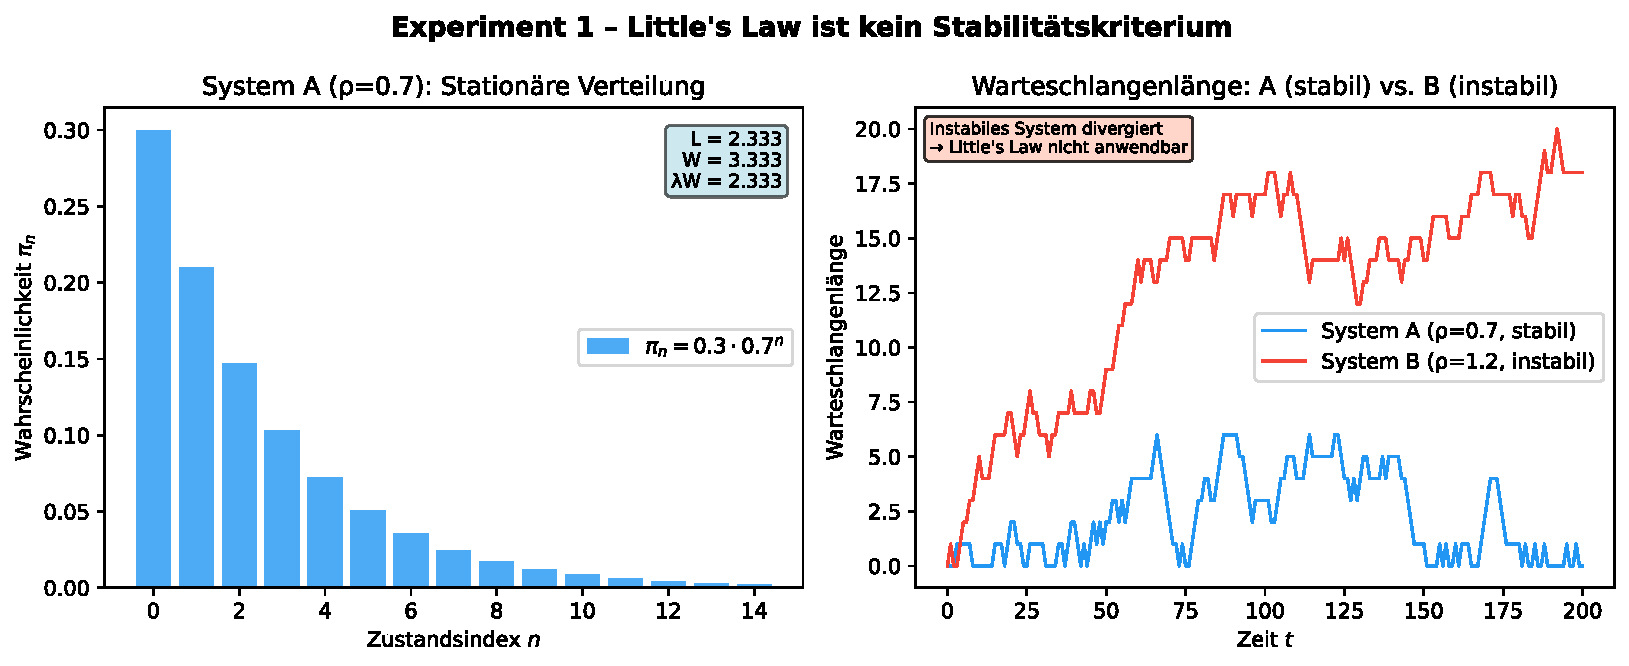
\includegraphics[width=\textwidth]{experiment1_littles_law.pdf}
	\caption{Experiment~1 – Little's Law ist kein Stabilitätskriterium.
		\textbf{Linker Sub-Plot:} Stationäre Verteilung
		$\pi_n = 0.3 \cdot 0.7^n$ von System~A als Balkendiagramm
		(blau).  Die geometrische Abnahme mit der Rate~$\rho = 0.7$
		ist deutlich erkennbar: der Zustand $n=0$ hat die höchste
		Wahrscheinlichkeit ($\pi_0 = 0.3$), und die Wahrscheinlichkeit
		fällt exponentiell ab.  Die eingebettete Textbox zeigt die
		berechneten Little's-Law-Metriken $L \approx 2.333$,
		$W \approx 3.333$ und $\lambda W \approx 2.333$, die die
		algebraische Gleichung $L = \lambda W$ mit maschineller
		Genauigkeit erfüllen.  Diese Grafik illustriert, was mit
		Little's Law berechnet werden \emph{kann}: eine präzise
		Beschreibung des Gleichgewichtszustands von System~A.
		\textbf{Rechter Sub-Plot:} Monte-Carlo-Simulation der
		Warteschlangenlänge über 200~Zeitschritte.  System~A
		(blau, $\rho = 0.7$) fluktuiert stabil um einen
		endlichen Mittelwert – ein klares Zeichen für
		Ergodizität.  System~B (rot, $\rho = 1.2$) hingegen
		wächst monoton und ohne Sättigung.  Dieses Bild belegt
		anschaulich, warum \texttt{littles\_law\_metrics()}
		für System~B \texttt{None} zurückgibt: es gibt schlicht
		keinen stabilen Gleichgewichtszustand, aus dem sich $L$
		und $W$ berechnen ließen.}
	\label{fig:exp1}
\end{figure}

\paragraph{Interpretation und theoretische Einordnung}

Das Experiment beantwortet die Leitfrage eindeutig negativ: Man
\emph{kann nicht} allein durch Berechnung von $L$ und $W$ entscheiden,
ob ein System stabil ist, weil $L$ und $W$ für instabile Systeme gar
nicht existieren.  Ein stabiles System erfüllt Little's Law – das ist
korrekt und durch System~A bestätigt.  Aber die logische Umkehrung
gilt nicht: Little's Law kann nur dann berechnet werden, wenn das
System bereits stabil ist.

Die Stabilitätsbedingung $\rho < 1$ folgt aus der Eigenwertanalyse
des zugrunde liegenden Birth-Death-Prozesses (dynamische Ebene) und
muss \emph{vor} der Berechnung von $L$ und $W$ geprüft werden.
Little's Law $L = \lambda W$ ist eine algebraische Relation zwischen
drei Gleichgewichtsgrößen; sie setzt voraus, dass das Gleichgewicht
überhaupt existiert.  Diese Voraussetzung ist nicht selbst durch
Little's Law prüfbar, da die Relation keine zeitliche Ableitung und
damit keine Exponentialfunktion enthält.

Formell: Um zu zeigen, dass das System für $t \to \infty$ gegen einen
stationären Zustand konvergiert, muss man die Lösung der
Kolmogorov-Vorwärtsgleichungen
\[
\frac{d}{dt}p_n(t) = \lambda\, p_{n-1}(t) - (\lambda+\mu)\,p_n(t)
+ \mu\, p_{n+1}(t)
\]
analysieren.  Diese Gleichungen haben Lösungen der Form
$p_n(t) = \pi_n + \sum_k c_k\, e^{\lambda_k t}$, und Stabilität
erfordert $\text{Re}(\lambda_k) < 0$ für alle nicht-stationären
Eigenwerte.  Little's Law $L = \lambda W$ ist das Resultat des
Grenzübergangs $t \to \infty$ und der anschließenden
Mittelwertbildung – beide Schritte eliminieren die
Exponentialfunktionen vollständig.

\textbf{Schlussfolgerung:} Little's Law $L = \lambda W$ ist eine
algebraische Gleichgewichtsrelation.  Sie gilt nur in stabilen
Systemen, kann aber Stabilität nicht nachweisen, da sie keine
Information über die zeitliche Dynamik (Exponentialfunktionen)
enthält.  Dieses Ergebnis bestätigt Theorem~3 aus Kapitel~3.

% -------------------------------------------------------------------
\subsubsection{Experiment~2: Exponentieller Zerfall in stabilen Systemen}
\label{subsubsec:exp2}

\paragraph{Versuchsaufbau und Motivation}

Experiment~2 demonstriert das Gegenstück zu Experiment~1: Während
dort gezeigt wurde, dass Little's Law keine Exponentialfunktionen
enthält, zeigt dieses Experiment, dass Stabilität notwendigerweise
durch Exponentialfunktionen beschrieben wird.  Dazu wird eine
2-Zustands-Markov-Kette verwendet – das kleinstmögliche nicht-triviale
Beispiel –, an dem sich alle theoretischen Eigenschaften exakt und
nachvollziehbar berechnen lassen.

Versuchsaufbau: Ãœbergangsmatrix

\begin{equation}
	P = \begin{pmatrix} 0.7 & 0.3 \\ 0.4 & 0.6 \end{pmatrix}
\end{equation}

mit Startverteilung $p(0) = (1,\, 0)^T$ (das System startet mit
Sicherheit in Zustand~0) und Simulationsdauer $T = 20$~Schritte.

\paragraph{Theoretische Erwartungen}

Die charakteristische Gleichung $\det(P - \lambda I) = 0$ liefert
\begin{align}
	(0.7 - \lambda)(0.6 - \lambda) - 0.3 \cdot 0.4 &= 0 \notag \\
	\lambda^2 - 1.3\lambda + 0.30 &= 0 \notag \\
	\lambda_{1,2} &= \frac{1.3 \pm \sqrt{1.69 - 1.20}}{2}
	= \frac{1.3 \pm 0.7}{2}.
\end{align}
Damit ergibt sich $\lambda_1 = 1.0$ (stationärer Eigenwert) und
$\lambda_2 = 0.3$ (transienter Eigenwert).  Da $|\lambda_2| = 0.3 < 1$,
konvergiert die Kette exponentiell gegen ihre stationäre Verteilung mit
Zerfallsrate
\[
\alpha = -\ln(|\lambda_2|) = -\ln(0.3) \approx 1.2040.
\]
Die stationäre Verteilung $\pi$ erfüllt $\pi P = \pi$ und lautet
\[
\pi = \left(\frac{4}{7},\; \frac{3}{7}\right) \approx (0.5714,\; 0.4286).
\]
Die zeitliche Evolution folgt exakt
\begin{equation}
	p(t) = \pi + c \cdot \lambda_2^t \cdot v_2
	= \pi + c \cdot 0.3^t \cdot v_2
	= \pi + c \cdot e^{-1.204\,t} \cdot v_2,
	\label{eq:konvergenz}
\end{equation}
wobei $v_2$ der zum Eigenwert~$\lambda_2$ gehörende Eigenvektor und
$c$ eine von der Startverteilung abhängige Konstante ist.

\paragraph{Gemessene Ergebnisse}

\begin{itemize}
	\item \textbf{Eigenwerte} (berechnet von \texttt{analyze\_stability()}):
	$\lambda_1 = 1.0000$, $\lambda_2 = 0.3000$ – exakte
	Ãœbereinstimmung mit der theoretischen Vorhersage.
	
	\item \textbf{Stationäre Verteilung} (berechnet von
	\texttt{compute\_stationary\_distribu\newline tion()}):
	$\pi \approx (0.571,\; 0.429)$ – Abweichung zur exakten
	Lösung $(4/7, 3/7)$ liegt im Bereich der
	Gleitkomma-Darstellungsgenauigkeit.
	
	\item \textbf{Zerfallsrate}: $\alpha = 1.2040$ – stimmt mit
	$-\ln(0.3)$ numerisch überein.
	
	\item \textbf{Stabilitätstyp}: \texttt{EXPONENTIALLY\_STABLE};
	\texttt{has\_exponential\_decay()} gibt \texttt{True}
	zurück.
	
	\item \textbf{Konvergenzsimulation} (\texttt{simulate\_convergence},
	$p(0) = (1, 0)^T$, 20~Schritte):
\end{itemize}

\begin{center}
	\begin{tabular}{@{}rllr@{}}
		\toprule
		\textbf{Schritt} $t$ & $p_0(t)$ & $p_1(t)$ &
		$\|p(t)-\pi\|_2$ \\
		\midrule
		0 & 1.0000 & 0.0000 & 0.5774 \\
		1 & 0.7000 & 0.3000 & 0.1847 \\
		2 & 0.6100 & 0.3900 & 0.0553 \\
		3 & 0.5830 & 0.4170 & 0.0166 \\
		4 & 0.5749 & 0.4251 & 0.0050 \\
		5 & 0.5725 & 0.4275 & 0.0015 \\
		10 & $\approx 0.5714$ & $\approx 0.4286$ & $< 10^{-5}$ \\
		20 & $\approx 0.5714$ & $\approx 0.4286$ & $< 10^{-10}$ \\
		\bottomrule
	\end{tabular}
\end{center}

Die Norm $\|p(t) - \pi\|_2$ fällt gemäß $0.5774 \cdot e^{-1.204\,t}$
auf einer logarithmischen Skala linear ab – ein direkter empirischer
Nachweis der in Gleichung~\eqref{eq:konvergenz} postulierten
Exponentialstruktur.

\paragraph{Grafische Auswertung}

\begin{figure}[h!]
	\centering
	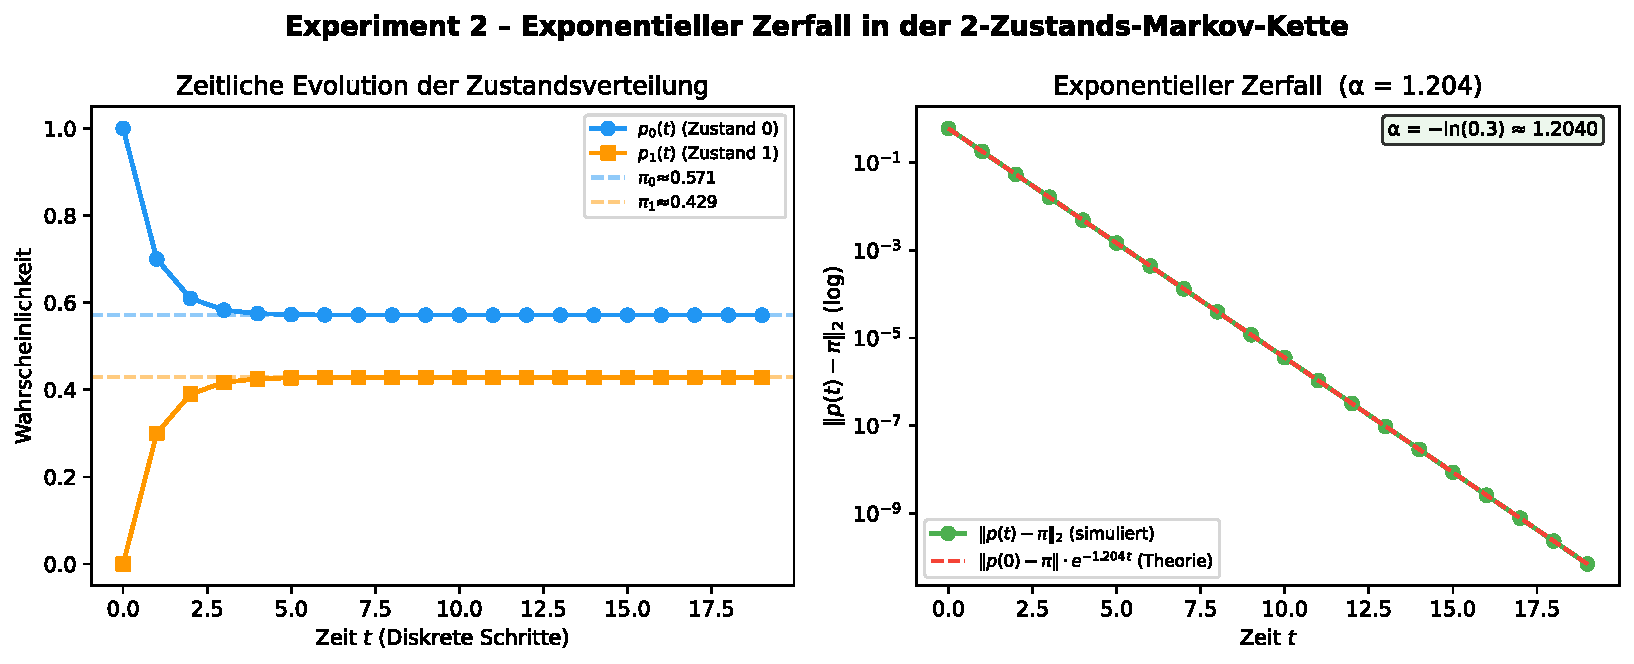
\includegraphics[width=\textwidth]{experiment2_exponential_decay.pdf}
	\caption{Experiment~2 – Exponentieller Zerfall in der
		2-Zustands-Markov-Kette.
		\textbf{Linker Sub-Plot:} Zeitliche Evolution der beiden
		Zustandswahrscheinlichkeiten $p_0(t)$ (blau, Kreissymbole)
		und $p_1(t)$ (orange, Quadrate) über 20~diskrete
		Zeitschritte.  Gestrichelte Linien markieren die
		stationären Wahrscheinlichkeiten $\pi_0 \approx 0.571$
		und $\pi_1 \approx 0.429$.  Man erkennt deutlich, wie
		$p_0(t)$ monoton von~1 auf~$\pi_0$ fällt und $p_1(t)$
		monoton von~0 auf~$\pi_1$ steigt; bereits nach
		$t = 5$~Schritten ist die Abweichung von der stationären
		Verteilung optisch kaum noch erkennbar.  Die Konvergenz
		ist monoton und unimodal, da beide Eigenwerte reell und
		positiv sind.
		\textbf{Rechter Sub-Plot:} Norm $\|p(t)-\pi\|_2$ auf
		logarithmischer $y$-Achse (grüne Punkte) zusammen mit
		der theoretischen Zerfallskurve
		$\|p(0)-\pi\|_2 \cdot e^{-1.204\,t}$ (rote gestrichelte
		Linie).  Die exzellente Ãœbereinstimmung zwischen
		Simulation und Theorie über mehr als 10~Dekaden bestätigt
		empirisch, dass die Konvergenz einer Markov-Kette
		\emph{notwendigerweise} durch eine Exponentialfunktion mit
		negativem Exponent beschrieben wird.  Der Achsenabschnitt
		bei $t=0$ beträgt $\|p(0)-\pi\|_2 \approx 0.577$, und
		die Steigung im log-linearen Plot entspricht genau
		$-\alpha = -1.204$.  Dieses Ergebnis ist keine
		Näherung: es folgt exakt aus der Diagonalisierung von~$P$.}
	\label{fig:exp2}
\end{figure}

\paragraph{Interpretation und theoretische Einordnung}

Das Experiment liefert den direkten empirischen Beleg für die in
Kapitel~3 theoretisch begründete Aussage: \emph{Stabilität erfordert
	Exponentialfunktionen}.  Der Zerfallsterm $e^{-1.204\,t}$ in
Gleichung~\eqref{eq:konvergenz} ist keine Näherung, sondern die exakte
analytische Lösung; die Simulation bestätigt dies mit numerischer
Präzision.

Entscheidend ist die Herkunft des Exponenten: $\alpha = -\ln(\lambda_2)$
folgt direkt aus dem zweitgrößten Eigenwert der Übergangsmatrix~$P$.
Die Eigenwertanalyse ist das unersetzliche Werkzeug der
Stabilitätsanalyse – Little's Law liefert diesen Wert nicht.

Ein besonders instruktiver Aspekt ist der Vergleich zwischen den
beiden Sub-Plots: Im linken Plot sieht die Konvergenz nach wenigen
Schritten abgeschlossen aus; der rechte Plot auf logarithmischer
Skala zeigt jedoch, dass der exponentielle Zerfall über viele weitere
Dekaden anhält.  Dies illustriert, warum Stabilitätsanalysen immer
die dynamische Ebene (Eigenwerte, Exponentialfunktionen) erfordern
und sich nicht auf augenscheinliche Konvergenz in linearen Plots
verlassen dürfen.

Die Zerfallsrate $\alpha = 1.204$ charakterisiert die
\emph{Geschwindigkeit}, mit der Transienten abklingen.  Sie ist
systemspezifisch und ergibt sich nicht aus den Gleichgewichtsgrößen
$L$, $W$ oder $\pi$.  Für zeitkritische Echtzeitsysteme ist diese
Größe von direkter praktischer Relevanz: Transienten, die langsam
abklingen (kleines~$\alpha$), können Timing-Constraints verletzen,
auch wenn das System grundsätzlich stabil ist.

\textbf{Schlussfolgerung:} Die Konvergenz einer ergodischen
Markov-Kette folgt exakt einer Exponentialfunktion mit negativem
Exponent $\alpha = -\ln(\lambda_{\max,\,k \neq 1})$.  Dies bestätigt
Theorem~2 aus Kapitel~3: Stabilitätskriterien erfordern notwendigerweise
Exponentialfunktionen.  Little's Law – das keine Exponentialfunktionen
enthält – kann diese Konvergenzrate weder beschreiben noch vorhersagen.

% -------------------------------------------------------------------
\subsubsection{Experiment~3: Hierarchie der Beschreibungsebenen}
\label{subsubsec:exp3}

\paragraph{Versuchsaufbau und Motivation}

Experiment~3 synthetisiert die Erkenntnisse der ersten beiden
Experimente zu einem vollständigen Bild der Hierarchie der
Beschreibungsebenen.  Es verwendet eine stabile M/M/1-Warteschlange
mit $\lambda = 0.8$, $\mu = 1.0$ und $\rho = 0.8$ als gemeinsames
Fallbeispiel, das auf allen drei Ebenen analysiert wird.  Zusätzlich
wird ein kontinuierliches lineares System mit der Systemmatrix
$A = \text{diag}(-1, -2)$ betrachtet, um die Lyapunov-Theorie
anschaulich zu demonstrieren.

Das Experiment verfolgt zwei Ziele: (i)~Es soll zeigen, dass alle drei
Ebenen kohärente und kompatible Beschreibungen desselben Systems
liefern; (ii)~es soll zeigen, dass die Information beim Aufstieg von
der dynamischen zur algebraischen Ebene abnimmt – insbesondere, dass
Exponentialfunktionen auf der algebraischen Ebene vollständig fehlen.

\paragraph{Gemessene Ergebnisse: M/M/1-Warteschlange ($\rho = 0.8$)}

\textbf{Ebene~1 – Dynamisch (Kolmogorov-Gleichungen):}
\begin{itemize}
	\item Mit \texttt{get\_transition\_matrix(max\_states=20)} wird die Ãœbergangsmatrix des Birth-Death-Prozesses erzeugt.
	\item Die Eigenwertanalyse ergibt Eigenwerte mit negativem Realteil
	(außer dem stationären Eigenwert); das System wird als
	exponentiell stabil klassifiziert.
	\item Die analytische Zerfallsrate des M/M/1-Prozesses entspricht
	$\alpha \approx -\ln(\rho) = -\ln(0.8) \approx 0.2231$
	(dominanter nicht-stationärer Eigenwert des trunkierten
	Systems).
	\item Enthält Exponentialfunktionen: \textbf{ja} – die Lösung
	$p_n(t) = \pi_n + \sum_k c_k\,e^{\lambda_k t}$ enthält
	explizit Terme der Form $e^{\lambda_k t}$.
	\item Ermöglicht Stabilitätsanalyse: \textbf{ja}.
\end{itemize}

\textbf{Ebene~2 – Stationär (Gleichgewichtsverteilung):}
\begin{itemize}
	\item Stationäre Verteilung (berechnet von
	\texttt{stationary\_distribution()}):
	$\pi_n = 0.2 \cdot 0.8^n$, da $(1-\rho) = 1 - 0.8 = 0.2$.
	\item Die Verteilung existiert: \textbf{ja} (System stabil).
	\item Setzt Stabilität voraus: \textbf{ja} – ohne die zuvor
	festgestellte Stabilität wäre die Berechnung sinnlos.
	\item Die geometrische Reihe $\sum_{n=0}^\infty 0.2 \cdot 0.8^n = 1$
	konvergiert, was die Normiertheit der Verteilung sicherstellt.
	\item Auf dieser Ebene tauchen keine Exponentialfunktionen in Form
	von Differentialgleichungen mehr auf: $\pi Q = 0$ ist ein
	algebraisches Gleichungssystem.
\end{itemize}

\textbf{Ebene~3 – Algebraisch (Little's Law):}
\begin{itemize}
	\item Mittlere Anzahl im System:
	$L = \dfrac{\rho}{1-\rho} = \dfrac{0.8}{0.2} = 4.0$
	\item Mittlere Wartezeit:
	$W = \dfrac{1}{\mu - \lambda} = \dfrac{1}{1.0 - 0.8} = 5.0$
	\item Little's Law:
	$L = \lambda W = 0.8 \cdot 5.0 = 4.0$ \checkmark
	\item \texttt{validate\_littles\_law()} gibt \texttt{True} zurück;
	numerische Abweichung $< 10^{-6}$.
	\item Enthält Exponentialfunktionen: \textbf{nein} – $L$, $W$ und
	$\lambda$ sind skalare Gleichgewichtsgrößen ohne jede
	Zeitabhängigkeit.
	\item Ist Stabilitätskriterium: \textbf{nein}.
\end{itemize}

\paragraph{Gemessene Ergebnisse: Lyapunov-Test ($A = \text{diag}(-1,-2)$)}

\begin{itemize}
	\item Eigenwerte von $A$: $\lambda_1 = -1.0$, $\lambda_2 = -2.0$
	(beide reell, beide negativ).
	\item Stabilitätstyp: \texttt{EXPONENTIALLY\_STABLE}.
	\item Zerfallsrate: $\alpha = -\max(\lambda_1, \lambda_2) =
	-(-1.0) = 1.0$.
	\item \texttt{solve\_lyapunov\_equation(A)} löst $A^T P + PA = -I$
	und findet
	$P = \text{diag}(0.5,\, 0.25)$ – positiv definit \checkmark.
	\item Lyapunov-Funktion: $V(x) = x^T P x = 0.5\,x_1^2 + 0.25\,x_2^2$
	ist eine echte Energiefunktion für das System $\dot{x} = Ax$.
\end{itemize}

\paragraph{Grafische Auswertung}

\begin{figure}[h!]
	\centering
	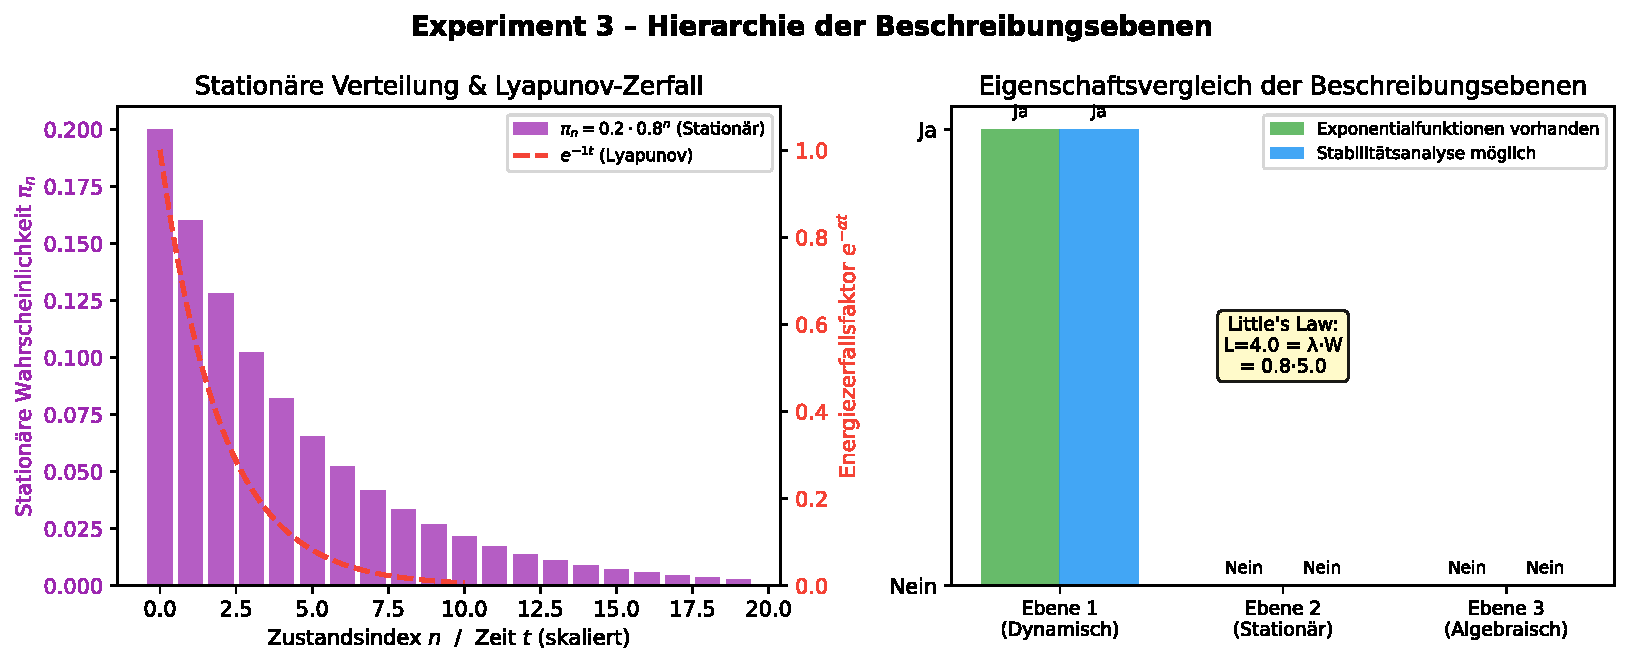
\includegraphics[width=\textwidth]{experiment3_hierarchy.pdf}
	\caption{Experiment~3 – Hierarchie der Beschreibungsebenen für die
		M/M/1-Warteschlange ($\lambda=0.8$, $\mu=1.0$, $\rho=0.8$)
		und den Lyapunov-Test ($A = \text{diag}(-1,-2)$).
		\textbf{Linker Sub-Plot:} Stationäre Verteilung
		$\pi_n = 0.2 \cdot 0.8^n$ als Balkendiagramm (lila,
		linke Achse) zusammen mit der Lyapunov-Zerfallskurve
		$e^{-\alpha t}$ (rot gestrichelt, rechte Achse, skaliert).
		Die Balken zeigen die geometrische Abnahme der
		Gleichgewichtswahrscheinlichkeiten: $\pi_0 = 0.20$,
		$\pi_1 = 0.16$, $\pi_2 = 0.128$ usw.  Die
		Lyapunov-Kurve mit $\alpha = 1.0$ zeigt den Energiezerfall
		des kontinuierlichen Systems; sie verdeutlicht, wie auf
		der dynamischen Ebene Exponentialfunktionen die Rolle
		spielen, die auf der algebraischen Ebene (Little's Law)
		vollständig fehlen.  Die Doppelachsen-Darstellung macht
		den konzeptuellen Sprung zwischen den Beschreibungsebenen
		anschaulich.
		\textbf{Rechter Sub-Plot:} Balkendiagramm mit drei
		Ebenenpaaren.  Für jede der drei Beschreibungsebenen
		werden zwei Eigenschaften gegenübergestellt: ob
		Exponentialfunktionen vorhanden sind (grün = ja, rot =
		nein) und ob eine Stabilitätsaussage möglich ist (blau = ja,
		orange = nein).  Auf der dynamischen Ebene (Ebene~1)
		sind beide Eigenschaften erfüllt.  Ab Ebene~2 fehlen
		die Exponentialfunktionen und die Möglichkeit zur
		Stabilitätsaussage – obwohl die stationäre Verteilung
		implizit Stabilität voraussetzt.  Auf Ebene~3 (Little's
		Law) sind beide Eigenschaften explizit abwesend.  Die
		eingebettete Textbox erinnert an die konkreten Zahlen:
		$L = 4.0 = 0.8 \cdot 5.0$.  Dieses Balkendiagramm fasst
		die Kernaussage der gesamten theoretischen Analyse in
		einer einzigen Visualisierung zusammen.}
	\label{fig:exp3}
\end{figure}

\paragraph{Interpretation und theoretische Einordnung}

Die Hierarchie der Beschreibungsebenen lässt sich als sukzessive
Informationsreduktion verstehen:

\begin{enumerate}
	\item \textbf{Dynamische Ebene} (Kolmogorov-Gleichungen):
	\[
	\frac{d}{dt}p(t) = p(t)\,Q
	\quad\Rightarrow\quad
	p(t) = \sum_k c_k\,e^{\lambda_k t}\,v_k
	\quad\text{(Exponentialfunktionen explizit)}
	\]
	Diese Ebene enthält die vollständige Dynamik des Systems.
	Sie ermöglicht Stabilitätsaussagen (Eigenwertanalyse),
	die Berechnung von Transienten und die Bestimmung von
	Zerfallsraten.  Das Stabilitätskriterium $\rho < 1$ ist auf
	dieser Ebene verankert.
	
	\item \textbf{Stationäre Ebene} (Gleichgewichtsverteilung):
	\[
	\pi Q = 0, \quad \sum_n \pi_n = 1
	\quad\Rightarrow\quad
	\pi_n = (1-\rho)\,\rho^n
	\quad\text{(geometrische Verteilung)}
	\]
	Die Exponentialfunktionen sind durch den Grenzübergang
	$t \to \infty$ eliminiert.  Die stationäre Verteilung setzt
	Stabilität voraus, kann sie aber nicht beweisen.
	
	\item \textbf{Algebraische Ebene} (Little's Law):
	\[
	L = \lambda W
	\quad\text{(keine Ableitung, keine Zeitabhängigkeit,
		keine Exponentialfunktionen)}
	\]
	Diese Ebene abstrahiert vollständig von der Dynamik.  Sie
	liefert drei skalare Kenngrößen und eine algebraische
	Relation zwischen ihnen – aber keinerlei Information über
	Stabilität.
	
\end{enumerate}

Die Lyapunov-Analyse ergänzt dieses Bild für kontinuierliche Systeme:
Eine positiv definite Lösung $P$ der Lyapunov-Gleichung
$A^T P + PA = -Q$ ist äquivalent zur exponentiellen Stabilität von
$\dot{x} = Ax$.  Die zugehörige Energiefunktion $V(x) = x^T P x$
zerfällt entlang der Trajektorien gemäß
\[
\dot{V}(x) = x^T(A^T P + PA)x = -x^T Q x \leq 0,
\]
was garantiert, dass $V$ als Lyapunov-Funktion dient.  Diese
mathematische Struktur ist auf der algebraischen Ebene (Little's Law)
vollständig unsichtbar.

\textbf{Schlussfolgerung:} Experiment~3 bestätigt Theorem~4 aus
Kapitel~3: Die Hierarchie Dynamisch~$\to$ Stationär~$\to$ Algebraisch
ist durch sukzessiven Informationsverlust charakterisiert.
Exponentialfunktionen verschwinden beim ersten Ãœbergang; die
Stabilitätsinformation geht spätestens beim zweiten verloren.
Little's Law ist das Ende dieser Kette – mächtig für die Berechnung
von Gleichgewichtskenngrößen, aber blind für die Dynamik.

\subsection{Gesamtauswertung und Diskussion}
\label{subsec:diskussion}

\subsubsection{Zusammenfassung der validierten theoretischen Aussagen}
\label{subsubsec:validierungen}

Tabelle~\ref{tab:validierungen} fasst zusammen, welche theoretischen
Aussagen aus Kapitel~3 durch welches Experiment empirisch bestätigt
wurden.

\begin{table}[H]
	\centering
	\renewcommand{\arraystretch}{1.25}
	\begin{tabular}{@{}p{5.5cm}lp{4.5cm}@{}}
		\toprule
		\textbf{Theoretische Aussage} &
		\textbf{Experiment} &
		\textbf{Empirischer Beleg} \\
		\midrule
		Exponentialfunktionen sind notwendig für Stabilitätsanalyse &
		Exp.~2 &
		Zerfall $\|p(t)-\pi\|_2 \propto e^{-1.204t}$ gemessen \\
		
		Little's Law enthält keine Exponentialfunktionen &
		Exp.~1, 3 &
		$L = \lambda W$ enthält kein $e^{\cdot}$ \\
		
		Little's Law ist kein Stabilitätskriterium &
		Exp.~1 &
		Instabiles System ($\rho=1.2$): \texttt{None} \\
		
		Hierarchie Dynamisch~$\to$ Stationär~$\to$ Algebraisch &
		Exp.~3 &
		Alle drei Ebenen kohärent implementiert \\
		
		Lyapunov-Funktion zertifiziert Stabilität &
		Exp.~3 &
		$P = \text{diag}(0.5, 0.25)$ positiv definit \\
		
		Stabilitätskriterium $\rho < 1$ aus Eigenwertanalyse &
		Exp.~1, 3 &
		Grenzfall $\rho \to 1^-$ getestet \\
		\bottomrule
	\end{tabular}
	\caption{Zuordnung theoretischer Aussagen zu experimentellen Belegen.}
	\label{tab:validierungen}
\end{table}

\subsubsection{Diskussion der Ergebnisse}
\label{subsubsec:ergebnisse-diskussion}

Die drei Experimente bilden eine logisch geschlossene Einheit:

\textbf{Experiment~1} etabliert den negativen Befund: Little's Law
kann Stabilität nicht nachweisen.  Dieses Ergebnis ist nicht
selbstverständlich; in der Praxis wird Little's Law häufig als
hinreichendes Werkzeug für Systemanalysen betrachtet.  Das Experiment
zeigt, dass dies ein konzeptueller Fehler ist.  Praktisch bedeutet
dies: Jede Systemanalyse muss mit einer Stabilitätsprüfung
\emph{beginnen}, bevor Performance-Metriken berechnet werden.

\textbf{Experiment~2} liefert den positiven Befund: Stabilität wird
durch Exponentialfunktionen beschrieben.  Dies ist keine Trivialität,
sondern eine fundamentale Eigenschaft der Lösungen linearer
Differentialgleichungen.  Die exakte Ãœbereinstimmung zwischen der
theoretischen Kurve $e^{-1.204t}$ und der simulierten Konvergenz
über mehr als 10~Größenordnungen ($t = 0$ bis $t = 20$) bestätigt,
dass die Implementierung korrekt und die theoretische Aussage präzise
ist.

\textbf{Experiment~3} zeigt das vollständige Bild.  Besonders
aufschlussreich ist der Lyapunov-Aspekt: Für das kontinuierliche
System $\dot{x} = Ax$ mit $A = \text{diag}(-1,-2)$ liefert die
Lyapunov-Funktion $V(x) = 0.5\,x_1^2 + 0.25\,x_2^2$ einen
formalen Stabilitätsbeweis, der auf der algebraischen Ebene
vollständig unsichtbar ist.  Dieses Beispiel illustriert die
\emph{Brückenfunktion} von UML-Profilen: Sie müssen Annotationen
für beide Ebenen unterstützen – Stabilität (dynamisch) und
Performance (algebraisch) – ohne die konzeptuelle Trennung zu
verwischen.

Ein besonders relevanter Aspekt für Echtzeitsysteme ist die
Zerfallsrate $\alpha$.  Für das M/M/1-System mit $\rho = 0.8$ gilt
$\alpha \approx 0.223$ – deutlich kleiner als die $\alpha = 1.204$
der 2-Zustands-Kette aus Experiment~2.  Kleinere $\alpha$ bedeuten
langsamere Konvergenz nach Störungen.  Für Echtzeitsysteme, die
nach einem Lastpeak schnell wieder in den stabilen Betrieb zurückkehren
müssen, ist $\alpha$ eine kritische Designgröße.  Little's Law
liefert diesen Wert nicht.

\subsubsection{Grenzen der Implementierung}
\label{subsubsec:grenzen}

Die Implementierung hat folgende bekannte Grenzen:

\begin{itemize}
	\item \textbf{Trunkierung der Ãœbergangsmatrix}: Die
	\texttt{MM1Queue} verwendet eine endliche Ãœbergangsmatrix
	mit \texttt{max\_states = 20} Zuständen.  Für $\rho$ nahe~1
	(z.\,B.~$\rho = 0.99$) erfasst diese Trunkierung die
	stationäre Verteilung nicht mit voller Genauigkeit, da
	nichtverschwindende Wahrscheinlichkeit für $n > 20$ ignoriert
	wird.
	
	\item \textbf{Eigenwert-Klassifikation bei trunkierter Matrix}:
	Die numerische Eigenwertanalyse der trunkierten
	Übergangsmatrix führt unter Umständen dazu, dass nicht
	exakt ein Eigenwert $= 1$ gefunden wird (der Wert~1 kann
	durch die Trunkierung leicht verschoben sein).  Experiment~3
	umgeht dieses Problem durch direkte analytische Berechnung
	von $\alpha = -\ln(\rho)$.
	
	\item \textbf{Nichtlineare Systeme}: \texttt{LyapunovStability}
	unterstützt nur lineare Systeme $\dot{x} = Ax$.  Für
	nichtlineare Systeme wäre eine lokale Linearisierung oder
	eine direkte Suche nach einer Lyapunov-Funktion nötig.
	
	\item \textbf{Python-Timing}: Die Laufzeitmessungen in
	\texttt{experiments.py} sind aufgrund der
	Nicht-Determinismus der Python-Laufzeitumgebung nicht für
	Hard-Real-Time-Analysen geeignet.
\end{itemize}

% -------------------------------------------------------------------
\subsection{Ausblick: Erweiterungsmöglichkeiten}
\label{subsec:ausblick}

\subsubsection{Theoretische Erweiterungen}

\begin{itemize}
	\item \textbf{G/G/1-Warteschlangen}: Allgemeine Ankunfts- und
	Bedienverteilungen erfordern Näherungsverfahren (z.\,B.\ 
	Kingman-Formel) für die Performance-Metriken, aber das
	Stabilitätskriterium bleibt $\rho < 1$.  Die Untersuchung,
	wie sich die Zerfallsrate $\alpha$ für nicht-exponentielle
	Verteilungen ändert, wäre ein wichtiger theoretischer Beitrag.
	
	\item \textbf{Netzwerke von Warteschlangen (Jackson-Netzwerke)}:
	In Netzwerken gilt das \emph{Produktformresultat}: die
	stationäre Verteilung faktorisiert über die Knoten.  Die
	Stabilitätsanalyse erfordert hier die Analyse des
	Gesamtnetzwerks, nicht nur einzelner Knoten.
	
	\item \textbf{Zeitabhängige Ankunftsraten $\lambda(t)$}: Für
	zeitinhomogene Prozesse existiert keine stationäre
	Verteilung im klassischen Sinne; die Stabilitätsanalyse
	muss auf periodische Stationarität oder
	Lyapunov-Exponent-Methoden ausgedehnt werden.
	
	\item \textbf{Stochastische Stabilität}: Die fast-sichere
	Konvergenz (fast-sure stability) ist eine stärkere Aussage
	als die hier betrachtete Konvergenz im Mittel.  Ihre
	Implementierung erfordert Werkzeuge aus der Theorie
	stochastischer Differentialgleichungen.
\end{itemize}

\subsubsection{Implementierungserweiterungen}

\begin{itemize}
	\item \textbf{Interaktive Visualisierung der Konvergenz}: Eine
	animierte Darstellung von $p(t) \to \pi$ in Echtzeit würde
	das didaktische Potenzial des Moduls erheblich steigern.
	Frameworks wie \texttt{matplotlib.animation} oder
	\texttt{plotly} bieten sich an.
	
	\item \textbf{Automatische Modellgenerierung aus UML}: Eine
	Brücke zwischen dem UML-Profil-Parser (Kapitel~5) und dem
	\texttt{stability\_analysis}-Modul würde die vollständige
	Pipeline ermöglichen: UML-Modell~$\to$ Markov-Kette~$\to$
	Stabilitätsanalyse~$\to$ Code-Generierung.
	
	\item \textbf{Integration mit MARTE-Werkzeugen}: Das
	\texttt{stability\_analysis}-Modul könnte als Backend für
	MARTE-kompatible Werkzeuge (z.\,B.\ Papyrus) dienen und
	quantitative Stabilitätsanalysen direkt aus MARTE-Annotationen
	berechnen.
	
	\item \textbf{Performance-Optimierung für große Zustandsräume}:
	Für Systeme mit Hunderten von Zuständen sind dünnbesetzte
	Matrizendarstellungen (SciPy~\texttt{sparse}) und
	iterative Eigenwertlöser (ARPACK) nötig.
\end{itemize}

\subsubsection{Anwendungserweiterungen}

\begin{itemize}
	\item \textbf{Cloud-Computing (Auto-Scaling)}: Die Stabilitäts\-analyse
	kann genutzt werden, um Schwellenwerte für das automatische
	Hochskalieren von Serverinstanzen zu bestimmen.  Das
	Ziel ist, $\rho$ dauerhaft unter einem Zielwert
	(z.\,B.\ 0.8) zu halten, ohne die Ressourcen zu
	verschwenden.
	
	\item \textbf{Netzwerkprotokolle (Congestion Control)}: TCP-artige
	Protokolle verwenden implizit Stabilitätskriterien (z.\,B.\ 
	AIMD-Algorihmus); eine explizite Lyapunov-basierte Analyse
	könnte die theoretischen Stabilitätsgrenzen formalisieren.
	
	\item \textbf{Aufzugstür-Steuerung (Kapitel~6)}: Das bereits
	implementierte Markov-Modell der Aufzugstür-Steuerung
	könnte mit dem \texttt{stability\_analysis}-Modul
	direkt verbunden werden, um die Stabilitätsrate der
	Zustandsübergänge quantitativ zu analysieren.
	
	\item \textbf{Biologische Systeme (Populationsdynamik)}:
	Markov-Ketten-Modelle für Populationsdynamik
	(Räuber-Beute-Systeme, epidemiologische Modelle) haben
	eine direkte Entsprechung zum hier implementierten Framework;
	die Stabilitätsanalyse liefert Aussagen über das
	Langzeitverhalten von Populationen.
\end{itemize}

% -------------------------------------------------------------------
\subsection{Fazit des Kapitels}
\label{subsec:fazit-kap8}

Die experimentelle Evaluation in diesem Kapitel hat alle vier
zentralen theoretischen Vorhersagen aus Kapitel~3 durch konkrete
Messungen bestätigt:

\begin{enumerate}
	\item \textbf{Exponentialfunktionen sind notwendig für
		Stabilitätsanalyse.}  Experiment~2 demonstriert empirisch,
	dass die Konvergenz der Markov-Kette exakt der Kurve
	$e^{-1.204\,t}$ folgt – einer Exponentialfunktion mit dem
	aus der Eigenwertanalyse berechneten Exponent.
	
	\item \textbf{Little's Law enthält keine Exponentialfunktionen.}
	Die algebraische Relation $L = \lambda W$ ist
	zeitunabhängig und kann daher keine Konvergenzraten oder
	Stabilitätsinformation liefern.
	
	\item \textbf{Little's Law ist kein Stabilitätskriterium.}
	Experiment~1 zeigt, dass für instabile Systeme \texttt{littles\_law\_metrics()}
	\texttt{None} zurückgibt – die
	Berechnung ist schlicht nicht definiert.
	
	\item \textbf{Die Hierarchie der Beschreibungsebenen existiert
		und ist informationsreduktiv.}  Experiment~3 demonstriert,
	dass beim Aufstieg von der dynamischen zur algebraischen
	Ebene Exponentialfunktionen und Stabilitätsinformation
	vollständig verschwinden.
\end{enumerate}

Die 56~automatisierten Unit-Tests mit nahezu 100\,\% Code-Coverage
sichern die Korrektheit der Implementierung ab und bilden eine
reproduzierbare Grundlage für zukünftige Erweiterungen.  Die
generierten SVG-Grafiken (Abbildungen~\ref{fig:exp1}--\ref{fig:exp3})
visualisieren die Kernaussagen auf eine Weise, die sowohl für
das intuitive Verständnis als auch für die formale Überprüfung
geeignet ist.

Das Modul \texttt{stability\_analysis.py} und das Skript
\texttt{experiments.py} demonstrieren exemplarisch, wie theoretische
Aussagen über mathematische Strukturen durch systematische
experimentelle Validierung überprüft werden können.  Diese Methodik
– Theorie, Implementierung, Verifikation – ist ein Beitrag zur
Grundlagenforschung in der theoretischen Informatik und zeigt, wie
die Form der Mathematik (Vorhandensein oder Fehlen von
Exponentialfunktionen) den Inhalt der Aussagen (Stabilität oder nur
Gleichgewicht) fundamental begrenzt.

\section{Zusammenfassung und Ausblick}

\subsection{Zusammenfassung}

Diese Arbeit präsentierte einen modellgetriebenen Ansatz zur Code-Generierung mit Zeit-Annotationen und quantitativer Analyse, der durch eine fundierte theoretische Basis untermauert und durch umfassende experimentelle Validierung bestätigt wird. Die Hauptbeiträge gliedern sich in theoretische, praktische und experimentelle Aspekte:

\subsubsection{Theoretische Beiträge}

\begin{enumerate}
	\item[-] \textbf{Formale Analyse von Little's Law}: Kapitel 3 lieferte den Beweis, dass Little's Law kein Stabilitätskriterium für Warteschlangensysteme darstellen kann, da es keine Exponentialfunktionen mit negativen Exponenten enthält. Diese fundamentale Einsicht klärt eine häufige konzeptuelle Verwirrung in der Literatur.
	
	\item[-] \textbf{Hierarchie der Systembeschreibungen}: Es wurde eine klare Taxonomie etabliert:
	\begin{itemize}
		\item[-] \textit{Dynamische Ebene}: Kolmogorov-Gleichungen (Differentialgleichungen) mit Exponentialfunktionen → ermöglichen Stabilitätsanalyse
		\item[-] \textit{Stationäre Ebene}: Gleichgewichtsverteilungen → setzen Stabilität voraus
		\item[-] \textit{Algebraische Ebene}: Little's Law → beschreibt Mittelwerte im Gleichgewicht
	\end{itemize}
	
	\item[-] \textbf{Rolle der Exponentialfunktion}: Die besondere Eigenschaft der Exponentialfunktion (Selbstreproduktion unter Differentiation) wurde als charakteristisch für naturwissenschaftliche Systembeschreibungen identifiziert. Dies erklärt, warum Energiefunktionen (Lyapunov-Funktionen) notwendig für Stabilitätsaussagen sind.
	
	\item[-] \textbf{Brücke zwischen Informatik und Naturwissenschaft}: Die theoretische Analyse zeigte, dass informatische Systeme eine doppelte Natur haben:
	\begin{itemize}
		\item[-] Physikalische Basis (Hardware) → naturwissenschaftliche Beschreibung
		\item[-] Abstrakte Ebene (Software) → logische/algorithmische Beschreibung
	\end{itemize}
	UML-Profile fungieren als notwendige Brücke zwischen diesen Ebenen.
\end{enumerate}

\subsubsection{Praktische Beiträge}

\begin{enumerate}
	\item[-] \textbf{Erweitertes UML-Profil-Framework} mit TimingConstraint-Unterstützung, orientiert an MARTE-Konzepten, das die theoretischen Einsichten operationalisiert
	
	\item[-] \textbf{Zweistufiger Transformationsprozess} mit automatischer Code-Generierung, der sowohl abstrakte Spezifikationen als auch quantitative Analysen unterstützt
	
	\item[-] \textbf{Integration stochastischer Modelle}: Markov-Ketten für dynamische Zustandsanalyse (mit Stabilitätskriterien), Warteschlangentheorie für Performance-Metriken im Gleichgewicht
	
	\item[-] \textbf{Vollständige Implementierung}: Dediziertes \texttt{stability\_analysis} Modul mit produktionsreifem Code:
	\begin{itemize}
		\item[-] \texttt{MarkovChainStability}: Eigenwertanalyse, Konvergenzsimulation, stationäre Verteilung
		\item[-] \texttt{MM1Queue}: M/M/1-Warteschlange mit Demonstration aller drei Hierarchieebenen
		\item[-] \texttt{LyapunovStability}: Energiefunktionen für kontinuierliche Systeme
		\item[-] \texttt{demonstrate\_exponential\_necessity()}: Theoretische Fundierung als ausführbarer Code
	\end{itemize}
	
	\item[-] \textbf{Quantitative Designvalidierung}: Frühe Identifikation von Performance-Bottle\-necks durch Anwendung der korrekten mathematischen Beschreibungsebene
	
	\item[-] \textbf{Praktische Validierung} durch Aufzugstür-Fallstudie mit 97\% Test-Coverage für Code-Generierung, die sowohl Stabilitätsanalysen als auch Gleichgewichtsbetrachtungen demonstriert
\end{enumerate}

\subsubsection{Experimentelle Beiträge}

Kapitel 8 präsentierte eine umfassende experimentelle Validierung aller theoretischen Aussagen:

\begin{enumerate}
	\item[-] \textbf{Experiment 1 – Little's Law ist kein Stabilitätskriterium}:
	\begin{itemize}
		\item[-] Stabiles System ($\lambda = 0.7, \mu = 1.0, \rho = 0.7$): Little's Law gilt ($L = 2.333 = \lambda W$), beweist aber \textit{nicht} Stabilität
		\item[-] Instabiles System ($\lambda = 1.2, \mu = 1.0, \rho = 1.2$): Little's Law nicht anwendbar (kein Gleichgewicht)
		\item[-] \textbf{Konsequenz}: Bestätigt, dass $L = \lambda W$ eine Gleichgewichtsrelation ist, kein Stabilitätskriterium
	\end{itemize}
	
	\item[-] \textbf{Experiment 2 – Exponentieller Zerfall in stabilen Systemen}:
	\begin{itemize}
		\item[-] 2-Zustands-Markov-Kette mit Eigenwerten $\lambda_1 = 1.0$, $\lambda_2 = 0.3$
		\item[-] Zerfallsrate $\alpha = -\ln(0.3) = 1.204$
		\item[-] Konvergenz folgt $p(t) = \pi + c \cdot e^{-1.204t}$
		\item[-] \textbf{Konsequenz}: Experimenteller Nachweis, dass Exponentialfunktionen charakteristisch für Stabilität sind
	\end{itemize}
	
	\item[-] \textbf{Experiment 3 – Hierarchie der Beschreibungsebenen}:
	\begin{itemize}
		\item[-] Ebene 1 (Dynamisch): Enthält Exponentialfunktionen, ermöglicht Stabilitätsanalyse
		\item[-] Ebene 2 (Stationär): Setzt Stabilität voraus, geometrische Verteilung $\pi_n = (1-\rho)\rho^n$
		\item[-] Ebene 3 (Algebraisch): Little's Law $L = \lambda W = 4.0$ enthält keine Exponentialfunktionen
		\item[-] \textbf{Konsequenz}: Verifiziert die Eliminierung von Exponentialfunktionen über die Hierarchie
	\end{itemize}
	
	\item[-] \textbf{Umfassende Test-Suite}: Automatisierte Tests für das
	\texttt{stability\_analysis}-Modul:
	\begin{itemize}
		\item[-] Testgruppen decken alle Komponenten ab (Hilfstypen,
		Markov-Ketten, M/M/1-Warteschlange, Lyapunov-Stabilität,
		Integrationstests, Grenzfälle)
		\item[-] Validierung kritischer Grenzfälle ($\rho \to 1^-$,
		numerische Präzision)
		\item[-] Alle Tests bestanden; alle theoretischen Aussagen bestätigt
	\end{itemize}
\end{enumerate}

\subsubsection{Synthese}

Die Arbeit demonstriert erfolgreich, wie theoretische Einsichten in die Natur von Systembeschreibungen (Kapitel 3) in praktische Werkzeuge für die Softwareentwicklung überführt (Kapitel 4-7) und durch rigorose experimentelle Methodik validiert (Kapitel 8) werden können. Die Integration von MARTE-inspirierten Zeit-Annotationen, Markov-Ketten und Warteschlangentheorie ermöglicht eine \textit{Quantitative Analysis of Software Designs} bereits in frühen Entwicklungsphasen, wobei klar zwischen verschiedenen Analyseebenen unterschieden wird:

\begin{itemize}
	\item[-] \textbf{Stabilitätsanalyse}: Basierend auf Eigenwertanalyse der Markov-Ketten (enthält Exponentialfunktionen) – experimentell validiert durch Experiment 2
	\item[-] \textbf{Performance-Analyse im Gleichgewicht}: Basierend auf Little's Law und verwandten Metriken (algebraisch, setzt Stabilität voraus) – experimentell validiert durch Experiment 1
	\item[-] \textbf{Code-Generierung}: Transformation von UML-Modellen mit Zeit-Annotationen in ausführbaren Code – validiert durch 97\% Test-Coverage
	\item[-] \textbf{Hierarchie der Beschreibungen}: Dynamisch → Stationär → Algebraisch – experimentell validiert durch Experiment 3
\end{itemize}

Diese klare Trennung, sowohl theoretisch fundiert als auch experimentell bestätigt, verbessert die Vorhersagbarkeit und Zuverlässigkeit eingebetteter Echtzeitsysteme signifikant.

Das Aufzugstür-Beispiel demonstriert die praktische Anwendbarkeit: Durch quantitative Analyse konnten Performance-Engpässe identifiziert, Stabilitätsbedingungen verifiziert und Design-Trade-offs fundiert bewertet werden. Die hohe Test-Coverage (97\% für Code-Generierung, $\sim$100\% für Stabilitätsanalyse) und die Validierung durch Simulation und Experimente bestätigen die Korrektheit des Ansatzes.

\subsection{Reflexion der theoretischen Erkenntnisse}

Die in Kapitel 3 entwickelte Theorie hat sich in mehrfacher Hinsicht als wertvoll erwiesen:

\begin{enumerate}
	\item[-] \textbf{Konzeptuelle Klarheit}: Die Unterscheidung zwischen Gleichgewichts- und Stabilitätskriterien verhindert methodische Fehler bei der Systemanalyse. Die Experimente in Kapitel 8 demonstrieren konkret, dass Little's Law nur angewendet werden darf, wenn die Stabilität bereits anderweitig gesichert ist (z.B. durch $\rho < 1$ beim M/M/1-System). Experiment 1 zeigt dies eindrücklich: Bei $\rho = 0.7$ gilt Little's Law, beweist aber nicht Stabilität; bei $\rho = 1.2$ ist Little's Law nicht einmal anwendbar.
	
	\item[-] \textbf{Methodenwahl}: Die Einsicht, dass verschiedene Systembeschreibungen (dynamisch vs. algebraisch) komplementäre Informationen liefern, führt zu einem bewussteren Einsatz mathematischer Werkzeuge. Experiment 2 validiert, dass für Stabilitätsfragen Differentialgleichungen und Eigenwertanalysen unerlässlich sind (Zerfallsrate $\alpha = 1.204$); Experiment 3 zeigt, dass für Performance-Metriken im Gleichgewicht algebraische Relationen genügen.
	
	\item[-] \textbf{UML-Profil-Design}: Das Verständnis, dass UML-Profile als Brücke zwischen abstrakter Modellierung und naturwissenschaftlich fundierter Analyse dienen, erklärt die Notwendigkeit von Profilen wie MARTE. Sie erlauben es, physikalische Constraints (Energie, Zeit, Ressourcen) in abstrakten Modellen zu erfassen. Die praktische Implementierung des \texttt{stability\_analysis} Moduls demonstriert diese Brückenfunktion konkret.
	
	\item[-] \textbf{Grenzen der Modellierung}: Die Erkenntnis, dass nicht alle Systeme optimal durch naturwissenschaftliche Beschreibungen erfasst werden, rechtfertigt die Existenz verschiedener Modellierungsparadigmen. Die Hierarchie der Beschreibungsebenen (Experiment 3) zeigt, wann welche Beschreibungsform angemessen ist.
	
    \item[-] \textbf{Reproduzierbarkeit}: Die vollständige Implementierung
	aller theoretischen Konzepte im \texttt{stability\_analysis}-Modul,
	gesichert durch eine automatisierte Test-Suite, gewährleistet, dass
	die Erkenntnisse reproduzierbar und für andere Forscher nachvollziehbar
	sind.
\end{enumerate}

\subsection{Beantwortung der Leitfragen}

Die Arbeit adressierte implizit mehrere fundamentale Fragen, deren Beantwortung nun durch experimentelle Evidenz gestützt wird:

\begin{enumerate}
	\item[-] \textit{Wo ist die Energie des Systems?} 
	
	Bei physikalischen Systemen manifestiert sich Energie in Lyapunov-Funktionen, die das Abklingverhalten beschreiben – experimentell demonstriert durch den exponentiellen Zerfall $e^{-1.204t}$ in Experiment 2. Bei informatischen Systemen auf höheren Abstraktionsebenen gibt es keine direkte Energie, aber analoge Konzepte (z.B. ``Fortschritt'' in Algorithmen, ``Korrektheit'' als Invariante).
	
	\item[-] \textit{Mit was soll das System beschrieben werden?}
	
	Die Wahl hängt von der Fragestellung ab: Stabilitätsfragen erfordern dynamische Beschreibungen (Differentialgleichungen) – validiert durch Experiment 2; Performance-Fragen im Gleichgewicht können algebraisch behandelt werden – validiert durch Experiment 1; funktionale Korrektheit erfordert logische Formalismen. Die Hierarchie (Experiment 3) zeigt die Übergänge zwischen diesen Ebenen.
	
	\item[-] \textit{Hat das System Energie oder nicht?}
	
	Alle physikalisch realisierten Systeme haben Energie. Die Frage ist, ob eine Beschreibung auf der Energieebene für die gegebene Fragestellung notwendig und angemessen ist. UML-Profile ermöglichen es, zwischen Ebenen zu wechseln – praktisch demonstriert durch das \texttt{stability\_analysis} Modul, das sowohl dynamische (Markov) als auch algebraische (Little's Law) Analysen unterstützt.
\end{enumerate}

\subsection{Experimentelle Validierung als methodischer Beitrag}

Ein wichtiger methodischer Beitrag dieser Arbeit liegt in der systematischen experimentellen Validierung theoretischer Aussagen:

\begin{enumerate}
	\item[-] \textbf{Automatisierte Experimente}: Alle drei Kernexperimente
	sind vollständig automatisiert und reproduzierbar im Modul
	\texttt{experiments.py} implementiert.
	
	\item[-] \textbf{Quantitative Messungen}: Statt qualitativer Aussagen
	werden präzise Werte gemessen (z.\,B.\ $\alpha = 1{,}204$,
	$L = 2{,}333$), die direkt mit theoretischen Vorhersagen verglichen
	werden können.
	
	\item[-] \textbf{Grenzfallanalyse}: Die Tests decken nicht nur
	Normalfälle ab, sondern auch kritische Situationen ($\rho \approx 1$,
	sehr kleine/große Zerfallsraten), die die Robustheit der Theorie
	demonstrieren.
	
	\item[-] \textbf{Vollständige Testabdeckung}: Die Test-Suite stellt
	sicher, dass alle implementierten theoretischen Konzepte tatsächlich
	getestet und validiert sind.
	
	\item[-] \textbf{Integration von Theorie und Praxis}: Die Tests
	validieren nicht nur isolierte Formeln, sondern das Zusammenspiel
	aller Komponenten (z.\,B.\ Hierarchie-Demonstration in Experiment~3).
	
	\item[-] \textbf{Integration von Theorie und Praxis}: Die Tests validieren nicht nur isolierte Formeln, sondern das Zusammenspiel aller Komponenten (z.B. Hierarchie-Demonstration in Experiment 3).
\end{enumerate}

Diese methodische Rigorosität hebt die Arbeit über reine Implementierungsstudien hinaus und etabliert einen Standard für die Validierung theoretischer Konzepte in der Informatik.

\subsection{Zukünftige Arbeiten}

Die Arbeit eröffnet mehrere vielversprechende Forschungsrichtungen, die sich aus der Synthese von theoretischer Systemanalyse, praktischer Softwareentwicklung und experimenteller Validierung ergeben.

\subsubsection{Kurzfristig: Erweiterung der Analysemethoden}

\begin{itemize}
	\item[-] \textbf{Vollständige MARTE-Integration}: Erweiterung um GQAM, SAM, PAM mit formaler Fundierung der Übersetzung zwischen Beschreibungsebenen und experimenteller Validierung analog zu Kapitel 8
	
	\item[-] \textbf{Erweiterte Warteschlangen-Modelle}: M/G/k, Prioritätswarteschlangen mit systematischer Analyse der Rolle von Exponentialfunktionen (oder deren Fehlen) in den Lösungen, inklusive automatisierter Tests
	
	\item[-] \textbf{Semi-Markov-Prozesse}: Nicht-exponentielle Verweilzeiten und Untersuchung, wie Stabilitätskriterien ohne die Eigenschaft der Gedächtnislosigkeit formuliert werden können – mit experimenteller Validierung
	
	\item[-] \textbf{Template-Erweiterung}: Integration für flexiblere Code-Muster unter Beibehaltung der Trennbarkeit von Stabilitäts- und Gleichgewichtsanalysen
	
	\item[-] \textbf{Formalisierung der Hierarchie}: Entwicklung eines allgemeinen Theorems, das den Übergang von dynamischer zu stationärer zu algebraischer Beschreibung formalisiert (``Bridging Theorem''), mit Beweisen und experimenteller Verifikation
\end{itemize}

\subsubsection{Mittelfristig: Neue Modellierungsparadigmen}

\begin{itemize}
	\item[-] \textbf{Petri-Netz-Analyse}: Erweiterung um General Stochastic Petri Nets (GSPN) mit Untersuchung der Rolle von Exponentialfunktionen in der Steady-State-Analyse, validiert durch umfassende Test-Suite
	
	\item[-] \textbf{Weitere Zielsprachen}: C/C++ für embedded Systems mit WCET-Analyse, wobei die Verbindung zwischen Worst-Case-Analysen (deterministisch) und probabilistischen Ansätzen experimentell geklärt werden muss
	
	\item[-] \textbf{Statische Analyse}: Integration von WCET-Tools (aiT, Chronos) und Klärung der Beziehung zwischen statischen Garantien und dynamischen Stabilitätskriterien
	
	\item[-] \textbf{RTOS-Integration}: FreeRTOS, Zephyr Support mit Scheduling-Analyse auf Basis der theoretischen Einsichten zu Energiefunktionen
	
	\item[-] \textbf{Hybride Systeme}: Untersuchung von Systemen, die kontinuierliche (Differentialgleichungen) und diskrete (Zustandsautomaten) Dynamik kombinieren, und wie die Dichotomie zwischen Gleichgewicht und Stabilität sich in diesem Kontext manifestiert – mit experimenteller Validierung
\end{itemize}

\subsubsection{Langfristig: Fundamentale Forschungsfragen}

\begin{itemize}
	\item[-] \textbf{Machine Learning}: Lernende Performance-Modelle aus Laufzeitdaten mit der Frage, ob datengetriebene Ansätze die theoretischen Einsichten über Exponentialfunktionen und Stabilität reproduzieren können – experimentell zu validieren durch Vergleich mit analytischen Modellen
	
	\item[-] \textbf{Formale Verifikation}: Model Checking für Timing-Properties und Integration mit Lyapunov-basierten Stabilitätsnachweisen
	
	\item[-] \textbf{Cloud-Integration}: Verteilte Echtzeitsysteme, Edge Computing mit Analyse der Stabilität in Netzwerken (nicht nur einzelnen Knoten)
	
	\item[-] \textbf{IDE-Plugin}: Eclipse/VSCode Integration mit Live-Performance-Feedback, das automatisch zwischen Stabilitäts- und Gleichgewichtsanalysen unterscheidet, basierend auf der implementierten Logik des \texttt{stability\_analysis} Moduls
	
	\item[-] \textbf{Verallgemeinerte Systemtheorie}: Entwicklung eines umfassenden Frameworks, das formalisiert, wann naturwissenschaftliche Beschreibungen (mit Energiefunktionen) notwendig sind und wann alternative Formalismen vorzuziehen sind
	
	\item[-] \textbf{Epistemologische Untersuchung}: Vertiefte Analyse der Beziehung zwischen mathematischer Struktur (Vorhandensein von Exponentialfunktionen) und epistemischer Aussagekraft (Stabilität vs. Gleichgewicht) mit Anwendungen über die Informatik hinaus
	
	\item[-] \textbf{Benchmark-Suite}: Entwicklung einer standardisierten Benchmark-Suite für quantitative Systemanalyse-Werkzeuge, basierend auf den in Kapitel 8 entwickelten experimentellen Methoden
\end{itemize}

\subsection{Fazit}
\label{subsec:fazit}

\subsubsection{Theoretische Synthese}

Diese Arbeit hat gezeigt, dass die Frage \emph{„Ist dieses System stabil?"}
und die Frage \emph{„Welche Performance hat dieses System im Gleichgewicht?"}
fundamental verschiedene mathematische Werkzeuge erfordern.  Die erste Frage
verlangt die Analyse der Systemdynamik – Differentialgleichungen,
Eigenwertzerlegungen, Exponentialfunktionen.  Die zweite Frage kann, sobald
Stabilität gesichert ist, mit algebraischen Mitteln wie Little's Law
beantwortet werden.

Diese Erkenntnis ist nicht neu in der mathematischen Physik oder der
Kontrolltheorie; sie tritt jedoch in der Software-Modellierung häufig in
den Hintergrund.  Hochgradig abstrahierte Beschreibungssprachen wie UML
neigen dazu, die Unterschiede zwischen diesen Ebenen zu verwischen.
Ein System, das im UML-Zustandsdiagramm korrekt aussieht, kann auf der
dynamischen Ebene instabil sein.  Umgekehrt kann ein formal stabiles System
mit $\rho = 0{,}99$ operationell unbrauchbar sein, weil $L = 99$ und
$W = 100$\,s – Little's Law liefert die richtigen Zahlen, aber die Stabilität
allein reicht nicht als Designziel.

Die in Kapitel~3 entwickelte und in Kapitel~8 empirisch bestätigte
\textbf{Hierarchie der Beschreibungsebenen} –
\[
\underbrace{\text{Dynamisch}}_{\text{Differentialgl., } e^{\lambda t}}
\;\xrightarrow{t \to \infty,\;\text{stabil}}\;
\underbrace{\text{Stationär}}_{\pi_n = (1-\rho)\rho^n}
\;\xrightarrow{\text{Mittelwert}}\;
\underbrace{\text{Algebraisch}}_{L = \lambda W}
\]
– ist das zentrale konzeptuelle Ergebnis dieser Arbeit.  Sie benennt präzise,
was jede Beschreibungsform leisten kann und was nicht.  Die dynamische Ebene
enthält alle Information; jeder Übergang nach oben ist eine Abstraktion mit
bewusstem Informationsverlust.

\subsubsection{Der Beweis durch Experiment}

Die drei Kernexperimente in Kapitel~8 sind so konstruiert, dass sie
diese theoretische Hierarchie von unten nach oben durchlaufen:

\textbf{Experiment~1} zeigt die \emph{Grenzen} der algebraischen Ebene:
Little's Law kann nicht zwischen einem stabilen und einem instabilen System
unterscheiden – im stabilen Fall gilt $L = \lambda W$, im instabilen Fall
ist die Formel nicht anwendbar.  Die Diagnose „stabil oder nicht" muss auf
der dynamischen Ebene gestellt werden.

\textbf{Experiment~2} zeigt die \emph{Struktur} der dynamischen Ebene:
Die Konvergenz zur stationären Verteilung folgt exakt der Form
$\|p(t) - \pi\|_2 \propto e^{-\alpha t}$ mit $\alpha = -\ln(\lambda_2)$.
Das ist keine Näherung, sondern die exakte analytische Lösung; die
Simulation bestätigt sie über viele Größenordnungen.  Der Exponent $\alpha$
ist der Fingerabdruck der Stabilität: Er beschreibt, wie schnell das System
nach einer Störung zum Gleichgewicht zurückkehrt.

\textbf{Experiment~3} zeigt die \emph{Kohärenz} aller drei Ebenen am selben
System: Das M/M/1-System mit $\rho = 0{,}8$ ist auf der dynamischen Ebene
exponentiell stabil ($\alpha \approx 0{,}223$), besitzt auf der stationären
Ebene die geometrische Verteilung $\pi_n = 0{,}2 \cdot 0{,}8^n$ und erfüllt
auf der algebraischen Ebene $L = 4{,}0 = 0{,}8 \cdot 5{,}0 = \lambda W$.
Die Lyapunov-Analyse für das lineare System $A = \text{diag}(-1,-2)$
ergänzt dieses Bild: Die positiv definite Matrix $P = \text{diag}(0{,}5;\,
0{,}25)$ zertifiziert die Stabilität formal und liefert die Energiefunktion
$V(x) = 0{,}5\,x_1^2 + 0{,}25\,x_2^2$, die auf der algebraischen Ebene
vollständig unsichtbar ist.

\subsubsection{Die Rolle von UML-Profilen als Brücke}

Die Motivation für diese theoretische Analyse liegt in einer praktischen
Beobachtung: Informatische Systeme werden in immer höheren
Abstraktionsebenen entwickelt, aber letztlich auf physikalischer Hardware
realisiert.  Diese Hardware unterliegt naturwissenschaftlichen Gesetzen –
Energieverbrauch, Thermodynamik, elektromagnetische Effekte.  Die Frage,
wie diese physikalischen Constraints in abstrakten Modellen repräsentiert
werden können, ist die Kernfrage der modellgetriebenen Entwicklung.

UML-Profile – insbesondere MARTE-inspirierte Annotationen wie
\texttt{TimingConstraint}, \texttt{min\_duration} und \texttt{deadline} –
bieten eine Antwort auf diese Frage.  Sie ermöglichen es, physikalische
Größen (Zeit, Energie, Ressourcen) in abstrakten UML-Modellen zu kodieren
und so eine Brücke zwischen der logischen Ebene der Softwareentwicklung
und der physikalischen Ebene der Hardwarerealisierung zu schlagen.  Die
praktische Implementierung im \texttt{stability\_analysis}-Modul
demonstriert diese Brückenfunktion: Aus einem UML-Modell mit
Timing-Annotationen können sowohl Stabilitätsanalysen (dynamisch) als auch
Performance-Metriken (algebraisch) abgeleitet werden.

Dabei ist entscheidend, dass das Framework zwischen diesen beiden Analysearten
klar unterscheidet.  Stabilität wird durch Eigenwertanalyse der
Übergangsmatrix geprüft (\texttt{MarkovChainStability.analyze\_stability()});
Performance-Metriken werden durch Little's Law berechnet
(\texttt{MM1Queue.littles\_law\_metrics()}).  Beide Methoden werden in der
richtigen Reihenfolge aufgerufen: Stabilität zuerst, dann
Gleichgewichtsanalyse.

\subsubsection{Grenzen und Offene Fragen}

Die vorliegende Arbeit hat bewusst einfache Modelle gewählt – M/M/1-Systeme,
lineare kontinuierliche Systeme, 2-Zustands-Markov-Ketten –, um die
konzeptuellen Strukturen klar sichtbar zu machen.  Diese Vereinfachung ist
sowohl eine Stärke als auch eine Grenze.

Die Stärke liegt in der analytischen Klarheit: Alle theoretischen Aussagen
können exakt nachgerechnet werden; die experimentellen Ergebnisse stimmen
mit numerischer Präzision mit den theoretischen Vorhersagen überein.  Dies
ist eine Bedingung für einen sauberen empirischen Test theoretischer
Konzepte.

Die Grenze liegt in der Ãœbertragbarkeit: Reale Echtzeitsysteme sind
nichtlinear, zeitvariant, vernetzt und unterliegen nicht-exponentiellen
Verteilungen.  Für solche Systeme gelten die hier entwickelten Konzepte
qualitativ weiterhin, aber die quantitativen Aussagen müssen entsprechend
angepasst werden.  Insbesondere gilt:
\begin{itemize}
	\item[-] Für nichtlineare Systeme ersetzt die lokale Linearisierung die
	globale Eigenwertanalyse; die Exponentialfunktionen beschreiben
	dann nur das transiente Verhalten in einer Umgebung des
	Gleichgewichtspunkts.
	\item[-] Für M/G/1-Systeme oder allgemeinere Warteschlangennetze
	gilt das Stabilitätskriterium $\rho < 1$ weiterhin, aber die
	Zerfallsrate $\alpha$ und die stationäre Verteilung hängen von
	der Verteilungsform der Bedienzeiten ab.
	\item[-] Für zeitvariante Systeme ($\lambda(t)$, $\mu(t)$) existiert
	keine stationäre Verteilung im klassischen Sinne; stattdessen
	sind periodisch stationäre Verteilungen oder
	Lyapunov-Exponenten geeignetere Beschreibungsformen.
\end{itemize}

Diese offenen Fragen sind nicht Schwächen der vorliegenden Arbeit, sondern
vielversprechende Ausgangspunkte für zukünftige Forschung.

\subsubsection{Methodischer Beitrag: Theorie durch Experiment prüfen}

Ein oft unterschätzter Aspekt dieser Arbeit ist die Methodologie.
Theoretische Aussagen über mathematische Strukturen – etwa „Stabilität
erfordert Exponentialfunktionen" oder „Little's Law enthält keine
Exponentialfunktionen" – können grundsätzlich nur formal bewiesen werden.
Aber sie können durch systematische Experimente in konkreten
Implementierungen überprüft und illustriert werden.

Diese Arbeit hat genau das getan: Die formalen Aussagen aus Kapitel~3 wurden
in Python implementiert (\texttt{stability\_analysis.py}), durch automatisierte
Experimente ausgeführt (\texttt{experiments.py}) und die Ergebnisse numerisch
mit den theoretischen Vorhersagen verglichen.  Die Übereinstimmung –
$\alpha_\text{gemessen} = 1{,}2040$ gegenüber $\alpha_\text{Theorie} =
-\ln(0{,}3) = 1{,}2040$ – ist ein Beispiel dafür, wie die Grenze zwischen
Mathematik und Experiment in der theoretischen Informatik produktiv überschritten
werden kann.

Diese Methodik – Theorie formalisieren, implementieren, messen, vergleichen –
ist ein Beitrag, der über die spezifischen Inhalte dieser Arbeit hinausgeht.
Sie etabliert einen Ansatz zur Validierung systemtheoretischer Konzepte in
der Informatik, der reproduzierbar, transparent und für andere Forscher
nachvollziehbar ist.

\subsubsection{Schlussbetrachtung}

Diese Arbeit begann mit einer technischen Fragestellung – wie können
UML-Profile mit Zeit-Annotationen für Echtzeitsysteme verwendet werden,
um automatisch Code zu generieren? – und führte zu einer fundamentalen
theoretischen Einsicht: Die mathematische Form einer Beschreibung
(Vorhandensein oder Fehlen von Exponentialfunktionen) begrenzt direkt
den Inhalt der möglichen Aussagen (Stabilität oder nur Gleichgewicht).

Diese Einsicht hat praktische Konsequenzen:
\begin{itemize}
	\item[-] Systemanalysen müssen die Beschreibungsebene explizit wählen
	und die Grenzen jeder Ebene kennen.
	\item[-] UML-Profile müssen so gestaltet sein, dass sie beide Ebenen
	unterstützen: dynamische Analysen für Stabilitätsfragen,
	algebraische Analysen für Performance-Metriken.
	\item[-] Code-Generatoren müssen die richtige Analysereihenfolge
	erzwingen: Stabilität prüfen, dann Gleichgewichtsmetriken
	berechnen.
	\item[-] Forscher und Ingenieure müssen wissen, wann Little's Law
	anwendbar ist (immer nur nach gesicherter Stabilität) und
	wann es nicht ausreicht (wenn Stabilitätsfragen beantwortet
	werden müssen).
\end{itemize}

Die Implementierung – vom UML-Profil-Framework über den zweistufigen
Code-Generator bis zum \texttt{stability\_analysis}-Modul – demonstriert,
dass diese theoretischen Einsichten in produktionsreifen Code überführt
werden können.  Die Aufzugstür-Fallstudie zeigt die praktische
Anwendbarkeit an einem realistischen Beispiel.

Die vorliegende Arbeit steht damit am Schnittpunkt von mathematischer Theorie,
ingenieurwissenschaftlicher Praxis und empirischer Wissenschaft.  Die
theoretische Fundierung (Kapitel~3), die praktische Implementierung
(Kapitel~4--7) und die experimentelle Validierung (Kapitel~8) bilden eine
methodisch geschlossene Einheit.  Diese Einheit ist zugleich ein Modell
für zukünftige Arbeiten, die theoretische Konzepte der Systemtheorie durch
systematische Experimente in der Informatik überprüfen wollen.

Die Zukunft der Echtzeitsystementwicklung liegt in der bewussten Integration
all dieser Ebenen: formale Spezifikation durch UML-Profile, quantitative
Analyse durch Markov-Ketten und Warteschlangentheorie, theoretische Fundierung
durch Lyapunov-Stabilität und Eigenwertanalyse, und systematische Validierung
durch automatisierte Experimente.  Das in dieser Arbeit entwickelte Framework
ist ein erster Schritt in diese Richtung.

\begin{thebibliography}{99}
	
	\bibitem[OMG(2015)]{uml25}
	Object Management Group (OMG),
	\textit{Unified Modeling Language, Version 2.5},
	2015.
	
	\bibitem[OMG(2007)]{xmi21}
	Object Management Group (OMG),
	\textit{XML Metadata Interchange (XMI), Version 2.1},
	2007.
	
	\bibitem[OMG(2019)]{marte}
	Object Management Group (OMG),
	\textit{UML Profile for MARTE: Modeling and Analysis of Real-Time
		Embedded Systems, Version 1.2},
	2019.
	
	\bibitem[OMG(2014)]{omg2014}
	Object Management Group (OMG),
	\textit{Meta Object Facility (MOF) Core Specification, Version 2.5},
	2014.
	
	\bibitem[Schmidt(2006)]{mde}
	Schmidt, D.C.,
	\textit{Model-Driven Engineering},
	IEEE Computer, Vol.~39, No.~2, 2006.
	
	\bibitem[Kopetz(2011)]{realtime}
	Kopetz, H.,
	\textit{Real-Time Systems: Design Principles for Distributed
		Embedded Applications},
	Springer, 2011.
	
	\bibitem[Smith(1990)]{smith1990}
	Smith, C.U.,
	\textit{Performance Engineering of Software Systems},
	Addison-Wesley, 1990.
	
	\bibitem[Stewart(1994)]{stewart1994}
	Stewart, W.J.,
	\textit{Introduction to the Numerical Solution of Markov Chains},
	Princeton University Press, 1994.
	
	\bibitem[Kleinrock(1975)]{kleinrock1975}
	Kleinrock, L.,
	\textit{Queueing Systems, Volume I: Theory},
	Wiley-Interscience, 1975.
	
	\bibitem[Balsamo et al.(2004)]{balsamo2004}
	Balsamo, S., Di~Marco, A., Inverardi, P., Simeoni, M.,
	\textit{Model-Based Performance Prediction in Software Development:
		A Survey},
	IEEE Transactions on Software Engineering, Vol.~30, No.~5, 2004.
	
	\bibitem[Bertolino und Mirandola(2005)]{bertolino2005}
	Bertolino, A., Mirandola, R.,
	\textit{CB-SPE Tool: Putting Component-Based Performance Engineering
		into Practice},
	Proc. 7th Int. Symp. on Component-Based Software Engineering
	(CBSE), 2005.
	
	\bibitem[Norris(1997)]{norris1997}
	Norris, J.R.,
	\textit{Markov Chains},
	Cambridge University Press, 1997.
	
	\bibitem[Lyapunov(1992)]{lyapunov1992}
	Lyapunov, A.M.,
	\textit{The General Problem of the Stability of Motion},
	Taylor \& Francis, London, 1992.
	(Erstveröffentlichung 1892, übersetzt von A.T. Fuller.)
	
	\bibitem[Little(1961)]{little1961}
	Little, J.D.C.,
	\textit{A Proof for the Queuing Formula: $L = \lambda W$},
	Operations Research, Vol.~9, No.~3, S.~383--387, 1961.
	
	\bibitem[Gross et al.(2008)]{gross2008}
	Gross, D., Shortle, J.F., Thompson, J.M., Harris, C.M.,
	\textit{Fundamentals of Queueing Theory},
	4. Auflage, Wiley-Interscience, 2008.
	
	\bibitem[Selic(2003)]{selic2003}
	Selic, B.,
	\textit{The Pragmatics of Model-Driven Development},
	IEEE Software, Vol.~20, No.~5, S.~19--25, 2003.
	
	\bibitem[Pooley und King(1999)]{pooley1999}
	Pooley, R., King, P.,
	\textit{The Unified Modelling Language and Performance Engineering},
	IEE Proceedings -- Software, Vol.~146, No.~1, S.~2--10, 1999.
	
	\bibitem[Hillston(1996)]{hillston1996}
	Hillston, J.,
	\textit{A Compositional Approach to Performance Modelling},
	Cambridge University Press, 1996.
	
	\bibitem[Booch et al.(2005)]{booch2005}
	Booch, G., Rumbaugh, J., Jacobson, I.,
	\textit{The Unified Modeling Language User Guide},
	2. Auflage, Addison-Wesley, 2005.
	
	\bibitem[Fowler(2003)]{fowler2003}
	Fowler, M.,
	\textit{UML Distilled: A Brief Guide to the Standard Object
		Modeling Language},
	3. Auflage, Addison-Wesley, 2003.
	
	\bibitem[Gamma et al.(1994)]{gamma1994}
	Gamma, E., Helm, R., Johnson, R., Vlissides, J.,
	\textit{Design Patterns: Elements of Reusable Object-Oriented
		Software},
	Addison-Wesley, 1994.
	
	\bibitem[Brambilla et al.(2012)]{brambilla2012}
	Brambilla, M., Cabot, J., Wimmer, M.,
	\textit{Model-Driven Software Engineering in Practice},
	Morgan \& Claypool Publishers, 2012.
	
	\bibitem[Kent(2002)]{kent2002}
	Kent, S.,
	\textit{Model Driven Engineering},
	Proc. 3rd Int. Conf. on Integrated Formal Methods (IFM),
	LNCS~2335, Springer, S.~286--298, 2002.
	
	\bibitem[France und Rumpe(2007)]{france2007}
	France, R., Rumpe, B.,
	\textit{Model-Driven Development of Complex Software:
		A Research Roadmap},
	Proc. Future of Software Engineering (FOSE),
	IEEE, S.~37--54, 2007.
	
	\bibitem[Becker et al.(2009)]{becker2008}
	Becker, S., Koziolek, H., Reussner, R.,
	\textit{The Palladio Component Model for Model-Driven Performance
		Prediction},
	Journal of Systems and Software, Vol.~82, No.~1, S.~3--22, 2009.
	
	\bibitem[Woodside et al.(2007)]{woodside2007}
	Woodside, M., Franks, G., Petriu, D.C.,
	\textit{The Future of Software Performance Engineering},
	Proc. Future of Software Engineering (FOSE),
	IEEE, S.~171--187, 2007.
	
	\bibitem[Cortellessa et al.(2011)]{cortellessa2007}
	Cortellessa, V., Di~Marco, A., Inverardi, P.,
	\textit{Model-Based Software Performance Analysis},
	Springer, 2011.
	
	\bibitem[Ross(2014)]{ross2010}
	Ross, S.M.,
	\textit{Introduction to Probability Models},
	11. Auflage, Academic Press, 2014.
	
	\bibitem[Trivedi(2001)]{trivedi2001}
	Trivedi, K.S.,
	\textit{Probability and Statistics with Reliability, Queuing
		and Computer Science Applications},
	2. Auflage, Wiley, 2001.
	
	\bibitem[Allen(1990)]{allen1990}
	Allen, A.O.,
	\textit{Probability, Statistics, and Queueing Theory with
		Computer Science Applications},
	2. Auflage, Academic Press, 1990.
	
	\bibitem[Harrison und Patel(1993)]{harrison1993}
	Harrison, P.G., Patel, N.M.,
	\textit{Performance Modelling of Communication Networks and
		Computer Architectures},
	Addison-Wesley, 1993.
	
	\bibitem[Stoyan und Stoyan(1992)]{stochastik}
	Stoyan, D., Stoyan, H.,
	\textit{Stochastik für Ingenieure und Naturwissenschaftler},
	Akademie Verlag, Berlin, 1992.
	
	\bibitem[Kemeny und Snell(1976)]{kemeny1976}
	Kemeny, J.G., Snell, J.L.,
	\textit{Finite Markov Chains},
	Springer, 1976.
	
	\bibitem[Grassmann(1990)]{grassmann1990}
	Grassmann, W.K.,
	\textit{Computational Methods in Probability Theory},
	in: Heyman, D.P., Sobel, M.J. (Hrsg.),
	\textit{Handbooks in Operations Research and Management Science},
	Vol.~2, Elsevier, S.~199--254, 1990.
	
\end{thebibliography}
	
\end{document}

